\documentclass[journal]{IEEEtran}
%\usepackage{float}
\usepackage[linesnumbered,ruled,vlined]{algorithm2e}
\usepackage{amssymb,amsmath}
\usepackage[font=small,skip=10pt]{caption}
\usepackage{subcaption}
\usepackage{comment}
\usepackage{color,soul}
\usepackage{ragged2e} 
\usepackage{algorithmicx}
\usepackage{algpseudocode}
\usepackage{amsthm}
\usepackage{cite}
\usepackage{array}
%\usepackage{nopageno}
\usepackage{url}
%\usepackage{hyperref}
%\usepackage{ulem}

% *** CITATION PACKAGES ***
%
\usepackage{cite}
\usepackage{color}
\usepackage{xspace}
\usepackage{multirow}
\usepackage{hhline}
%\usepackage[pdftex]{graphicx}

% *** GRAPHICS RELATED PACKAGES1 ***
%

% more space
%\usepackage{txfonts}
\addtolength{\abovedisplayskip}{-2mm}
\addtolength{\belowdisplayskip}{-2mm}
\addtolength{\parskip}{-.15mm}
%\addtolength{\arraycolsep}{-.75mm}
\addtolength{\abovecaptionskip}{-1mm}
\addtolength{\belowcaptionskip}{-1mm}
%\renewcommand{\baselinestretch}{0.9}


\ifCLASSINFOpdf
\usepackage[pdftex]{graphicx}
\graphicspath{{fig/}{../}}
\DeclareGraphicsExtensions{.pdf,.jpeg,.png,.jpg}
\else
\usepackage[dvips]{graphicx}
\graphicspath{{fig/}{../}}
\DeclareGraphicsExtensions{.eps}
\fi

%\usepackage[caption=false,font=footnotesize]{subfig}
%
% correct bad hyphenation here
\hyphenation{op-tical net-works semi-conduc-tor}
%\setlength{\intextsep}{-1ex} % remove extra space above and below in-line float


\renewcommand{\baselinestretch}{1}

\ifodd 1
\newcommand{\rev}[1]{{\color{black}#1}}%revise of the text
\newcommand{\revv}[1]{{\color{black}#1}}%revise of the text
\newcommand{\com}[1]{\textbf{\color{red}(COMMENT: #1)}}%comment of the text
\else
\newcommand{\rev}[1]{#1}
\newcommand{\com}[1]{}
\fi


\newcolumntype{L}[1]{>{\raggedright\let\newline\\\arraybackslash\hspace{0pt}}m{#1}}
\newcolumntype{C}[1]{>{\centering\let\newline\\\arraybackslash\hspace{0pt}}m{#1}}
\newcolumntype{R}[1]{>{\raggedleft\let\newline\\\arraybackslash\hspace{0pt}}m{#1}}

%\newcommand{\opt}{\textsc{OPT}\xspace}
\newcommand{\sa}{\textsc{SmartAllocate}}
\newcommand{\rc}{\textsc{ReConsider}}
\newcommand{\bc}{\textsc{BetaCover}}
\newcommand{\ics}{\textsc{iCS}\xspace}
\newcommand{\fcs}{\textsc{fCS}\xspace}
\newcommand{\MCSP}{\textsf{SPAN}\xspace}
\newcommand{\dMCSP}{\textsf{dSPAN}\xspace}
\newcommand{\focs}{\textsc{foCS}\xspace}
\newcommand{\iocs}{\textsc{ioCS}\xspace}
\newcommand{\finalalg}{\textsc{ioCS+}\xspace}
\newcommand{\opt}{\textsc{OPT}\xspace}
\newcommand{\alg}{\textsc{ALG}\xspace}
\newcommand{\rtl}{\textsc{GreedyRTL}\xspace}
\newcommand{\iolp}{\textsc{ioLP}\xspace}
\newcommand{\folp}{\textsc{foLP}\xspace}

\newcommand{\be}{\begin{equation}}
	\newcommand{\ee}{\end{equation}}
\newcommand{\bee}{\begin{eqnarray}}
	\newcommand{\eee}{\end{eqnarray}}
\newcommand{\bse}{\begin{subequations}}
	\newcommand{\ese}{\end{subequations}}
%\def\bee#1\eee{\begin{align}#1\end{align}}
\newcommand{\nnb}{\nonumber}

\newtheorem{lem}{Lemma}
\newtheorem{propos}{Proposition}
\newtheorem{thm}{Theorem}
\newtheorem{defi}{Definition}


%in terms of practical feasibility and characterizing the maximum benefits of D2D load balancing is
\newtheorem{theorem}{Theorem}[section]
\newtheorem{lemma}[theorem]{Lemma}
\newtheorem{proposition}[theorem]{Proposition}
\newtheorem{corollary}[theorem]{Corollary}

\makeatletter
\newcommand\semiHuge{\@setfontsize\semiHuge{22.52}{27.38}}
\makeatother
\begin{document}
	%\semiHuge
	\title{Online EV Scheduling Algorithms for Adaptive Charging Networks with Global Peak Constraints}
	\author{\#}
	
	\author{Bahram Alinia, Mohammad H. Hajiesmaili, Zachary J. Lee, Noel Crespi, and Enrique Mallada
		
		\thanks{ B. Alinia and N. Crespi are with the department of Networks and Mobile Multimedia Services (RS2M), Institut Mines-Telecom,
			Telecom SudParis, Evry, France (e-mail: bahram.alinia@telecom-sudparis.eu, noel.crespi@mines-telecom.fr).
			
			M. H. Hajiesmaili and E. Mallada are with the Department of Electrical and Computer Engineering, Johns Hopkins University, Baltimore, MD, USA (e-mail: \{hajiesmaili,mallada\}@jhu.edu).

			Z. J. Lee is with the Department of Electrical Engineering, California Institute of Technology, Pasadena, CA, USA (e-mail: zlee@caltech.edu).
		} }
		
		\maketitle

\begin{abstract}
%			With the rapid growth of electric vehicles, their high demand charging jobs pose an immense challenge to the grid infrastructure. 
			This paper tackles online scheduling of electric vehicles (EVs) in an adaptive charging network (ACN) with local and global peak constraints. Given the aggregate charging demand of the EVs and the peak constraints of the ACN, it might be infeasible to fully charge all the EVs according to their charging demand. Two alternatives in such resource-limited scenarios are to maximize the social welfare by partially charging the EVs (fractional model) or selecting a subset of  EVs and fully charge them (integral model). 
%			This paper tackles both fractional and integral models. 
			The critical challenge is the need for online solution design since in practical scenario\revv{s} the scheduler has no information of future arrivals of EVs in a time-coupled underlying problem. 
			For the fractional model, we devise both offline and online algorithms. We prove that the offline algorithm is optimal. Using competitive ratio as the performance measure, we prove the online algorithm achieves a competitive ratio of 2. The integral model, however, is more challenging since the underlying problem is NP-hard due to 0/1 selection criteria of EVs. Hence, efficient solution design is challenging even in offline setting. We devise a low-complexity primal-dual scheduling algorithm that achieves a bounded approximation ratio. Built upon the offline approximate algorithm, we propose an online algorithm and analyze its competitive ratio in special cases. Extensive trace-driven experimental results show that the performance of the proposed online algorithms is close to the offline optimum, and outperform the existing solutions. 
%			\rev{In particular, the grid and electricity providers should be aware of the electricity peak.	It is known in electricity market that the spot price is a dominating factor in billing cost. Hence, the utility companies need to identify a global peak constraint for the cost management purpose. This paper studies the online EV charging scheduling problem in a utility that offers EV charging service in a set of CSs, each of which having limited output power (referred to as local peak constraint) while taking into account the global peak constraint. The scheduling problem in this scenario comes with unique challenges that is not tackled previously.}


%			\rev{The problem objective is to maximize total revenue of the CSs.} 

\end{abstract}
		\begin{IEEEkeywords}
			Electric Vehicle, Online Scheduling, Approximation Algorithm, Competitive Analysis
		\end{IEEEkeywords}		

		\section{Introduction}
\label{sec:intro}	
%		\IEEEPARstart{A}{s} 
%		a result of global warming and environmental concerns through dependence on fossil fuels, there has been a rapid proliferation in deploying renewable energy sources. 
\IEEEPARstart{T}{o} promote quick adoption of renewable energy sources, electrification of vehicles is a trend that has been globally advocated in recent years. \rev{According to a Bloomberg report, EVs will account for more than half of the new car sales by $2040$~\cite{bloomberg}. 		
	%the global sale of EVs increased by $80\%$ in $2015$~\cite{EVSales}.
	%		With the significant advantage of electric vehicles (EVs) in being an environment friendly product, the global interest for EVs is rapidly growing, such that  
	Consequently, it is expected that demand from EV charging will constitute a considerable portion of total demand. 
	Currently, transportation consumes $29\%$ of total energy in the US, while electricity production consumes $40\%$~\cite{Zhao}.} 
%Vehicles seen accounting for 5\% of electricity use by $2040$~\cite{EVSales2}}
%%%\revv{\sout{Hence, rapid electrification of the vehicles makes the total electricity demand of EVs significant.}} 

\revv{EV charging demand is a typical example of a deferrable load, and there is often considerable flexibility in the charging schedule. This property makes the problem of EV charging scheduling  important and there is an extensive research along this direction in the literature (see the recent survey~\cite{mukherjee2015review}, and references therein). In most of the existing works, the EV charging demand is treated as a constraint to the problem in a low-load regime~\cite{Tang}.  Motivated by rapid proliferation of EVs, this work tackles the EV scheduling in high-load regime, where given the aggregate charging demand of the EVs and the peak constraints of the charging network, it is not feasible to fully charge all the EVs according to their charging demand.}
%		\subsection{Microgrid: Definition, Potentials, and Challenges}
%		\label{sec:introA}
%		A common trend in the smart grid era is to install renewable energy sources in distributed manner. More specifically, medium or large commercial and industrial  customers such as universities, headquarters, etc.,  can take control of their own energy consumption by local deployment of renewable sources~\cite{Hajiesmaili2016Online}. In this setting, the residual demand, i.e., total demand subtracted by the local renewable supply, can be acquired from the external grid. 

%		In addition to clean energy production, the owner of microgrid also enjoys more power sustainability and reliability, and the ability to proactively manage the energy costs.  


More specifically, this paper studies resource-constrained EV charging scheduling in an adaptive charging network (ACN) governed by a single operator in a campus-scale location such as a university, a headquarter\rev{s}, etc. \cite{wu2017two}. 
\rev{A notable example is the Caltech ACN~\cite{lee2016adaptive} where individual charging ports are organized into several \textit{charging stations} (CSs) which are dispersed in a \textit{charging network}} with the capability of adaptive charging of the EVs. 
The problem is different from EV charging scheduling \revv{with capacity constraint} in single station scenarios~\cite{Tang,Wen,Shroff2014,WTang,Chen,Xiang,Zhao,Robu} (we refer to~Section~\ref{sec:rel} for detailed discussions on related work), because of the essential need to respect the aggregate peak demand of the ACN. \revv{Note that, the ACN operator might limit the total power drawn from EVs to control costs~\cite{PeakPrice,Zhang2015eEnergy}, reserve the capacity for other loads, and/or participate in demand-response programs.}
%		The EV charging loads are usually flexible and deferrable, which means that their load can be scheduled~\cite{moghaddam2017smart,DWang} to shape the total demand over time. 
%The aim of this paper is to use the deferrable property of EVs and schedule their charging jobs, so as to \rev{maximize the revenue of the ACN}.	
%		We refer to Section~\ref{sec:rel} for the literature review. 	

%		In particular, real-world pricing scheme for large customers is usually a hybrid time-of-use and peak-based charging model where the peak demand can significantly impact the total energy cost, e.g., the peak price is often more than $100$ times higher than the spot price~\cite{PeakPrice,Zhang2015eEnergy}. Considering total aggregate demand, the peak charge portion could be as large as $20\%-80\%$ of total cost~\cite{Xu2014Reducing}. Consequently, a substantial cost reduction could be achieved if the total peak-demand can be proactively controlled \cite{liao2015dispatch}. 

%		\subsection{EV Charging Scheduling in the ACN}
%		With the proliferation of EVs, the charging requirement of the microgrid EVs could be a portion of total microgrid electricity demand. 


%		To respond the electricity demand of EVs, CSs are being used where EVs can recourse to charge their battery \cite{He,liao2015dispatch,Tang}. There can be few to many CSs dispersed in an ACN, e.g., each for a parking garage of a building in a university campus. In this scenario, all parking stations are governed by a facility operator and a \textit{global} peak demand constraint is determined such that the aggregate charging demand in the entire network is less than this global peak demand \cite{DWang,Hoog}.

%		The charging scheduling of the EVs with the goal of respecting the \textit{global aggregate peak constraint}, however, is a unique problem which is different from the single station EV charging scheduling. Most of the existing work in the literature, tackle the problem in the single parking station scenario. We refer to Section~\ref{sec:rel} for in-depth discussion. As discussed in Section \ref{sec:problem}, the global optimal solution cannot be obtained by separately solving the single station problems. 
%		On the other hand, there are only a few studies that provide global optimal solution for charging scheduling of EVs \cite{He, Moradijoz, Malhotra,Zeng,Shaaban,DWang}. Despite elegant results, the underlying problems, e.g., charging cost minimization problem in \cite{He}, average operating cost minimization with optimal electricity exchange capacity problem in \cite{DWang}, optimal station capacity problem in~\cite{Moradijoz}, user convenience maximization problem in~\cite{Malhotra}, joint optimization of system profit and user experience in~\cite{Shaaban,Zeng} are different from the problem studied in this paper.

%		\subsection{Problem, Challenges, and Contributions}
We consider a scenario with multiple EVs where each EV has different charging profile in terms of availability, charging demand, charging rate limit, and valuation of getting charged \revv{(for details see Section~\ref{sec:ev})}. We formulate an online EV charging scheduling problem with the goal of \textit{selecting} and \textit{scheduling} a subset of EVs such that: (1) the charging demand of the selected EVs are (fully or partially) satisfied; (2) the charging rate limit of EV batteries are respected, (3) the global peak constraint of the ACN is satisfied~\cite{lee2016adaptive}; (4) the local peak constraint of each CS is respected;  and finally, (5) the total revenue obtained by the valuation of the EVs is maximized. 



%		of maximizing the revenue of the ACN. The constraints are the \textit{local} peak constraint of each CS, and the \textit{global} peak constraint that limits the accumulative charging demand drawn from the entire network of stations (decided by the administration of the ACN to control total peak demand~\cite{lee2016adaptive}). 

There are two main challenges in the design and implementation of scheduling algorithms for EVs satisfying the goals mentioned above. \rev{Firstly, the problem calls for online scheduling design.} In practice, EVs arrive to the CS in online fashion and the scheduler has no information about the arrival and demand of the future EVs. Secondly, the underlying optimization problem in integral model is NP-hard even in offline case \rev{(see Section~\ref{sec:integral})}. This is because the problem is a mixed integer linear problem and a ``time-expanded'' extension of knapsack problem which is known as a classic NP-hard problem. In this paper, we tackle the challenge of online design by following competitive algorithm design~\cite{borodin2005online} and the challenge of NP-hardness by pursuing approximation algorithm design~\cite{approx} and make the following contributions: 

$\vartriangleright$ We first consider a \textit{fractional model} (where EVs can be charged partially and the revenue is proportional accordingly) and design an optimal offline scheduling algorithm. 
%In addition to provide efficient result, the algorithm has a further elegant step to apply a valley filling strategy to further reduce the peak demand of EV charging without degrading total revenue. 
We then develop an efficient online algorithm in which no exact or stochastic information about the future EV arrivals is given. Despite its simplicity, the algorithm is proved to be $2$-competitive with optimal offline solution, i.e., the revenue of the proposed online algorithm is at least $1/2$ of the offline optimum, regardless of input sequence. 
Even though there are competitive algorithms in the literature for similar problems, to the best of our knowledge, our algorithm is the first $2$-competitive algorithm \rev{which considers the} charging rate limits.

$\vartriangleright$ We next study \rev{the} more challenging scenario of \rev{the} \textit{integral model}\rev{, }where EVs must receive all their demand to make revenue. We first propose a polynomial-time primal-dual offline approximate algorithm. We analyze the approximation ratio of the algorithm and by strengthening the linear relaxed version of the mixed integer problem~\cite{Carr}, we obtain an approximation ratio of $\alpha =1+\sum_{j=1}^m {\frac{p_j}{p_j-q_j}}.\frac{s}{s-1}$, where $p_j$ is local peak constraint in station $j$, $q_j$ is the maximum charging rate of the EVs in station $j$ and $s$ is a slackness parameter. We highlight that when $p_j \gg q_j$ and $s$ is \rev{large} enough, then $\alpha \approx m+1$, where $m$ is the number of stations in the ACN. Built on the basis of the offline algorithm, we devise an online algorithm, and discuss its competitive ratio in special cases. 
%In particular, the competitive ratio is $b\Big(1+\frac{p_j}{p_j-q_j}\cdot\frac{s}{s-1}\Big)$ for single station scenario, where $b$ is the number of batches with the same arrival time.

$\vartriangleright$ We conduct a set of  simulations to evaluate the performance of our proposed algorithms. 
%For offline scheduling problem under integral charging model, the results  demonstrate that the proposed approximation algorithm is close to the optimal solution and is significantly better than the obtained theoretical bounds. 
The results of online algorithms for both integral and fractional settings are close to the optimum (within $90\%$ and $94\%$ for integral and fractional models in a representative scenario). In addition, our algorithm outperforms the existing scheduling algorithm in Caltech ACN~\cite{lee2016adaptive} by $35\%$ for integral revenue model.
%The simulation section also discusses on the positive and negative effects of slackness parameter in different scenarios. 

%To the best of our knowledge, this problem is not addressed yet in previous studies. 

%		\subsection{Paper Organization}
%		The rest of this paper is organized as follows. Section~\ref{sec:rel} reviews the literature. In Section \ref{sec:model}, the system model  and problem formulation are described. 
%		Section \ref{sec:fractional} provides offline and online algorithms for fractional model. We study integral model in Section \ref{sec:integral} and propose online and offline algorithms. The simulation results are reported in Section~\ref{sec:simul}. Section~\ref{sec:conclusion} concludes the paper and highlights future directions.	

\section{Related Work}
\label{sec:rel}
\revv{There is an extensive work in the general topic of EV demand management and scheduling~\cite{mukherjee2015review} by considering different scenarios such as optimal operations with EV coordinations~\cite{mukherjee2017distributed}, EV scheduling with incorporation of renewable energy, and energy storage systems~\cite{de2017impact,shafie2018innovative}. In this section, we focus on the literature related to peak-constrained EV charging scheduling in single and multiple stations.}
\subsubsection{Peak-Constrained EV Charging Scheduling}
\label{sec:rel:peakconstrained}			
\revv{There is an extensive literature on EV charging scheduling problem focusing on single CS~\cite{Tang,Wen}, while the local and global peak constraints are omitted or only the local peak is considered.}	As we discuss in Section~\ref{sec:problem}, the global optimal solution cannot be obtained by separately solving the single station problems. Hence, those solutions cannot be directly applied to the multiple CS scenario with global peak constraints. 

%A scenario that local and global peak constraints exist is the case that scheduling is required for a charging network for multiple CSs. 
Studies in \cite{He,malhotra2017distributed,Moradijoz,DWang,Zeng,Shaaban} tackled charging scheduling problem in multiple CSs. The authors in~\cite{He} studied a global cost minimization EV charging scheduling problem. However, there is no limit on the maximum peak demand that the system can tolerate. Consequently, the peak can be arbitrary high and beyond the physical limit of the transformers in the charging station~\cite{lee2016adaptive} leading to huge electricity bills~\cite{Zhang2015eEnergy}. Besides, the charger devices installed in the CSs have limitation on the maximum power that they can transfer in each time unit~\cite{Tesla}. 
%We solve the issue by constraining local and global peaks. However, to meet the peak constraints, it may not be feasible to respond to all charging demands. Consequently, only a subset of EVs can be charged~\cite{Xiang}, which is captured in our problem formulation. 
\cite{DWang} considered a multi-microgrid system with global peak constraint where each microgrid has a CS and the goal is to manage electricity exchange between microgrids and main grid to minimize the operating costs. The authors assume that required information about individual EVs is available by forecast which may not represent a real scenario. A similar assumption is made in \cite{Zeng,Shaaban} where the objective is to maximize total utility of EVs and aggregators in a distribution network.
%\rev{To be removed: In our solution, we applied a priority based selection process (based on the EVs' valuation) to respond to the demands to make sure that total peak respects the constraints. The selection process can be made based on different criteria such as the value of each charging request \cite{Lee, Xiang} or the priority.}
%To avoid big billing cost in peak hours, \cite{Moradijoz} proposed a solution based on genetic algorithm to find optimal capacity and location of parking lots for serving demands in peak hours with the goal of maximizing total benefit of all stations. Although authors studied the problem under multiple CS setting, their solution is not applicable to our setting when the CSs are already set up. 
The authors in~\cite{malhotra2017distributed} use a similar model as in this paper, where both local and global peak constraints are considered. However, the authors solve the single-slot problem, which fails to provide a general solution taking into account EVs' arrival and departure times as considered in our study.
Finally, as an alternative approach to control the peak, some studies directly target minimizing the peak~\cite{Zhao, Karfopoulos}. In~\cite{Zhao}, an online algorithm is developed for EV charging to minimize the peak and \cite{Karfopoulos} proposed a valley filling method by leveraging V2G in peak hours. Although the peak is minimized in above works, it cannot guarantee that the minimized peak is tolerable by the underlying charging network.


\subsubsection{Scheduling Under Demand Uncertainty}
A main challenge in EV scheduling problem is to cope with demand uncertainty. Many studies including \cite{Shroff2014,Tang,WTang,Chen,Xiang,Zhao,Robu} addressed online scheduling problem with different objectives. \cite{Shroff2014,Xiang} studied the problem of maximizing social welfare considering the benefit for both users and service provider. \cite{Tang} and \cite{WTang} developed algorithms to minimize the charging price for the CS, where the proposed algorithm in \cite{Tang} is $2.39$-competitive. 
%An online algorithm developed in \cite{Chen} to optimize overall operating profit of the service provider. 
In \cite{Robu}, an online $2$-competitive algorithm is proposed for a single CS, assuming that EVs are capable of being discharged in a negligible amount of time. The assumption, however, is not realistic for EVs.

Our problem in this paper is unique from above works in many respects. First, we study the problem in an ACN where several CSs exist, while none of the above studies solve the problem under this setting. Second, the previous algorithms do not work for both integral and fractional charging models. In addition, \cite{WTang,Chen} put no limit on the charging rate of EVs which makes their solution impractical in real scenarios. Also, \cite{WTang,Tang, Shroff2014,Chen,Zhao} do not consider the peak limit of the CS. 
\revv{Note that some studies~\cite{jin2017optimal} tackle the scenarios of satisfying the large demands (possibly EV demands) by participating in electricity market. This study assumes that the electricity price is given and fixed, and leaves the case of real-time pricing as the future direction. In addition, there are studies that incorporate prediction in online EV charging scheduling~\cite{wang2017predictive,chen2014distributional}. The prediction-based approaches achieve satisfactory performance for the scenarios that follow prediction. Deviation from prediction models, however, degrades their performance. Our approach, on the other hand, has no assumptions on modeling/prediction, and in this way, is robust against any uncertainty in the instances to the problem.} 
\revv{Finally, in~\cite{Alinia2018ITS}, we considered a simplified EV charging scheduling in fractional model without global peak constraints and devised heuristic algorithms (without competitive and approximation analysis) with on-arrival commitment for EVs to notify the amount that they can receive by their departure. }
%In this paper, we consider these limitations and develop online and offline algorithms for fractional and integral revenue models in an ACN and provide theoretical bounds on their performance.



%It is important to note that there is a considerable similarity between EV scheduling problem and classical job scheduling problem \cite{}. However, most algorithm developed for job scheduling problem  do not consider a limit on processing rate of the jobs. 

%\cite{Shroff2014} and \cite{Stein2012} study social welfare maximization problem while the profit of both EV owners and CS is considered.  social welfare of the EV owners \cite{Stein2012}, charging cost \cite{Tang,WTang}, and total value of fully charged EVs \cite{Azar}). In addition, \cite{WTang, Tang,Shroff2014,Zhao} do not take into account the peak limitation of CS. }
		\section{System Model and Problem Formulation}
		\label{sec:model}
		
		
		
		\subsection{System Model}
		We consider a time-slotted system model in which the time horizon is divided to $T$ equal length slots ${t=\{1, 2, \dots ,T\}}$ (e.g., $T=24$ with time slots of $1$ hour length).
\subsubsection{Charging Network}
\label{sec:acn}
Our charging network model is inspired by the Caltech ACN~\cite{lee2016adaptive} as illustrated in Fig.~\ref{fig:model-a}. In \rev{the} Caltech EV charging network (located in a parking garage), electricity is distributed through a two-level transformer architecture from a main switch panel to multiple EV switch panels (\rev{$2$} panels in the current Caltech ACN). Each EV switch panel then is connected to several chargers ($\approx$25 chargers \rev{per panel} in the Caltech ACN). The total power drawn from the main switch panel \rev{by} the charging network has a power limit of  $p^\mathsf{total}$, that is determined by the facility operator to control the costs, reserve the capacity for other loads, and/or participate in demand-response programs.  
%This power, where we refer to it as \emph{network power limit} is used for both EV charging as well as non-EV charging purposes (e.g., lighting, fans, etc \cite{lee2016adaptive}). 
In other words, $p^\mathsf{total}$, which we refer to it as the \textit{global peak}, hereafter, limits the maximum aggregate EV charging load at each time slot. 
%The global peak must be less than or equal to the value obtained by subtracting non-EV load from network power limit. 
%When we write \emph{global peak constraint}, it refers to $p^\mathsf{total}$.  
%$p^\mathsf{total}$ is the maximum allowed aggregated electricity consumption by all stations at each slot and limits the total transferable power to EVs. 

We assume that there are $m$ EV switch panels that represent $m$ CSs. In addition to the global peak constraint, each CS $j$ has \rev{a} capacity constraint on \rev{its} total power drawn, indicated by $p_j$, and referred to it as the \emph{local peak} constraint. The \rev{value of} $p_j$ is determined by the output power limit of the transformers installed between the main switch panel and EV switch panels and could be different for each EV switch panel.  
%installed chargers in a CS have limited output power to charge EVs ~\cite{Wen,Xiang,Tesla}. Therefore, for CS $j$, $p_j$ cannot be more than sum of output power of its chargers. 
\rev{It is often observed that the charging demand of different CSs (EV switch panels in Fig.~\ref{fig:model-a}) are well below the local peak constraints.}
To increase the flexibility due to heterogeneous charging demand of CSs, in the Caltech ACN, the global peak constraint of the main switch can be \textit{over-provisioned}, i.e., $p^\mathsf{total}$ is less than the aggregate local peaks,  ($\sum_j p_j\geq p^\mathsf{total}$). \rev{While this increases flexibility, it also couples the problem of EV charging scheduling across different CSs.}
%Despite increased flexibility, the over-provisioning property, however, couples the problem of EV charging scheduling across different CSs. 
Our solutions in this paper will be centralized ones which can be obtained through communication between the CSs and a central server as illustrated in Fig. \ref{fig:model-b}.


%We make this clear by a simple example. Assume $m=2, p^\mathsf{total}=50$ kW and $p_1=p_2=25$ kW. In a specific time slot (e.g., $t=1$), the total demand in CS $1$ and $2$ is $40$ kWh and $10$ kWh, respectively. According to local peak constraints, it is not feasible to satisfy all demands in a single time slot. However, if we had $p_1=p2=50$ kW (e.g., by installing more chargers in the stations) we could be able to satisfy all demands by allocating $40 kW$ in $p_1$ and $10 kW$ in $p_2$ while still not violating $p^\mathsf{total}$. In case that $\sum_j p_j\leq p^\mathsf{total}$, the scheduling problem is not challenging and the solution can be obtained by solving the problem locally in each CS. If $\sum_j p_j> p^\mathsf{total}$ (which is the case we consider in this paper), a centralized solution is needed that can be obtained through communication between the CS and a central server as illustrated in Fig. \ref{fig:model-b}. 


\begin{figure}	
\centering
\minipage{0.49\textwidth}
				\begin{subfigure}[b]{0.69\textwidth}
					\begin{center}
						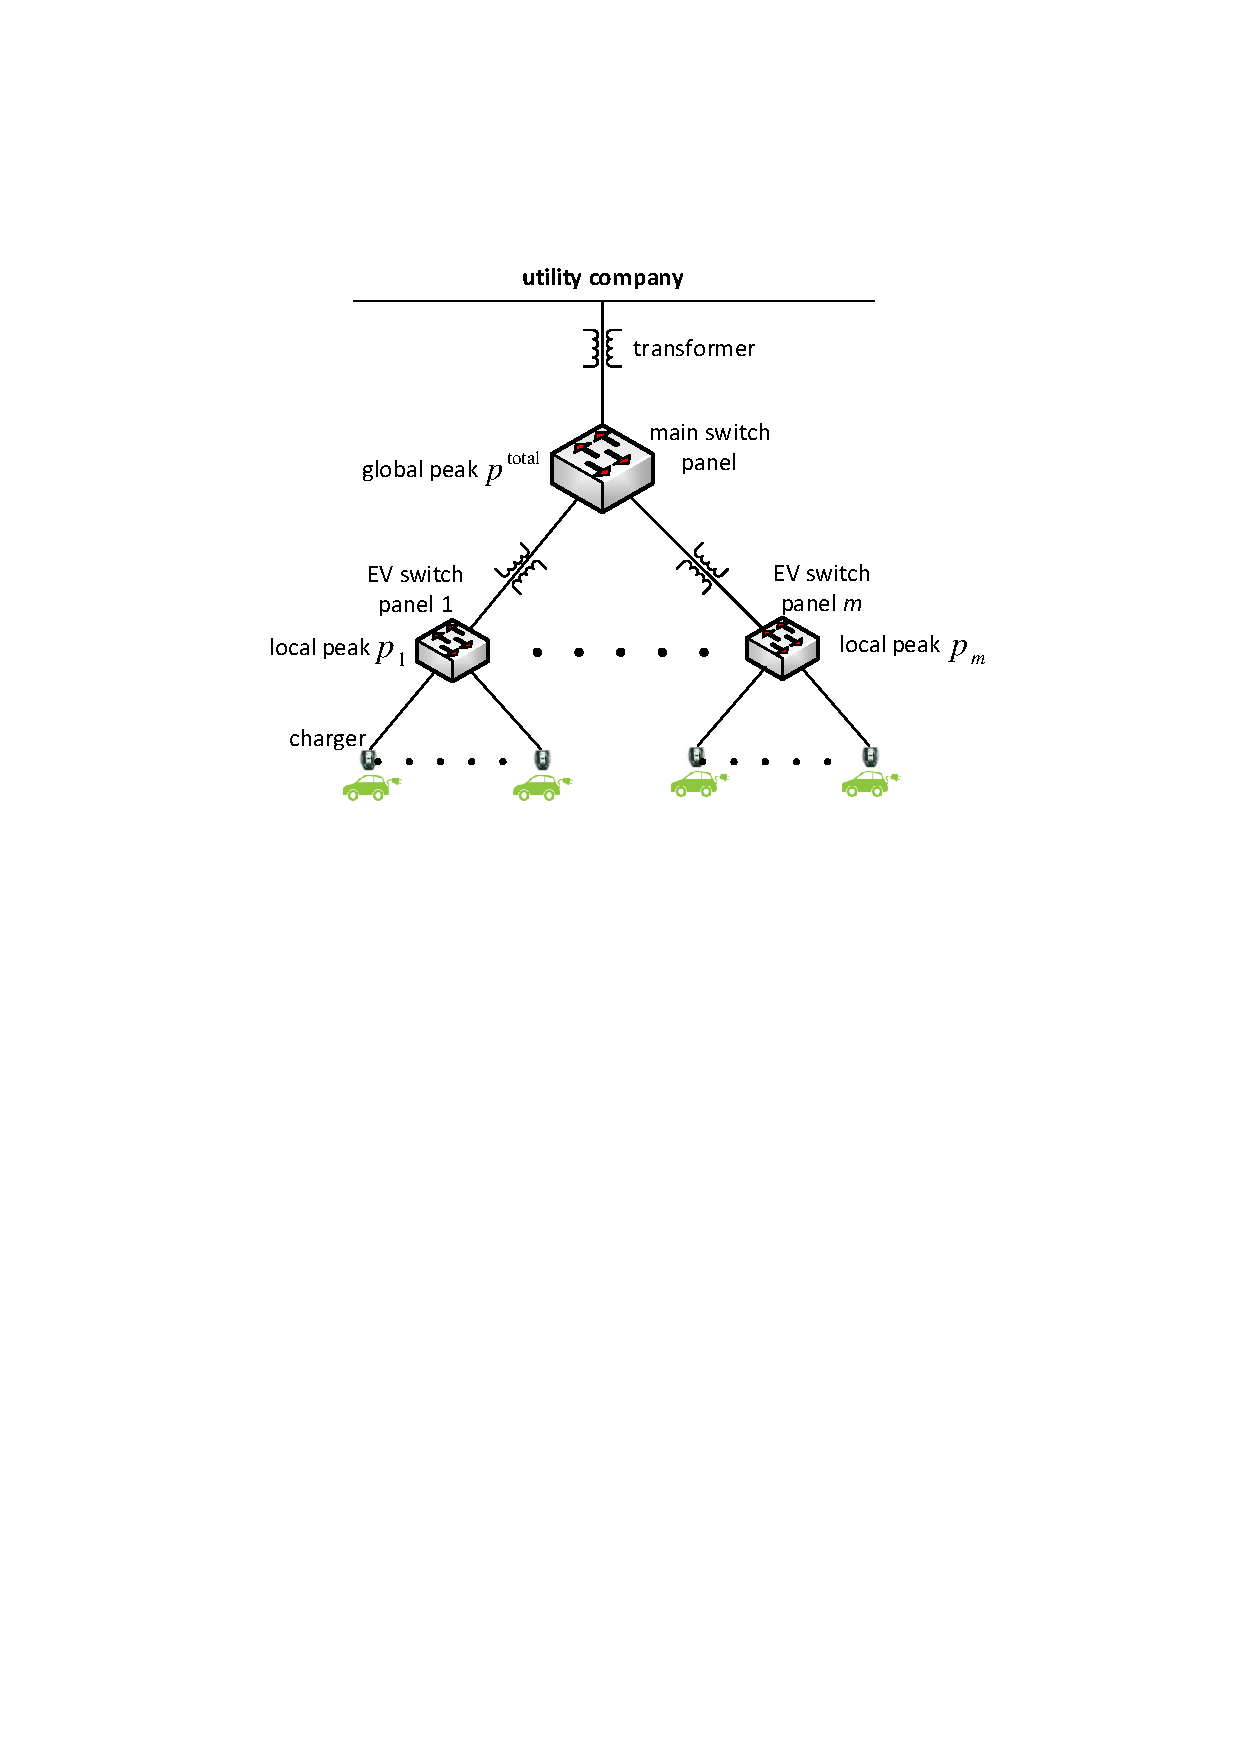
\includegraphics[width=\textwidth]{model-a.pdf}
						\caption{Caltech adaptive charging network (ACN)}
						\label{fig:model-a}
					\end{center}
				\end{subfigure}%
				\begin{subfigure}[b]{0.29\textwidth}
					\begin{center}
						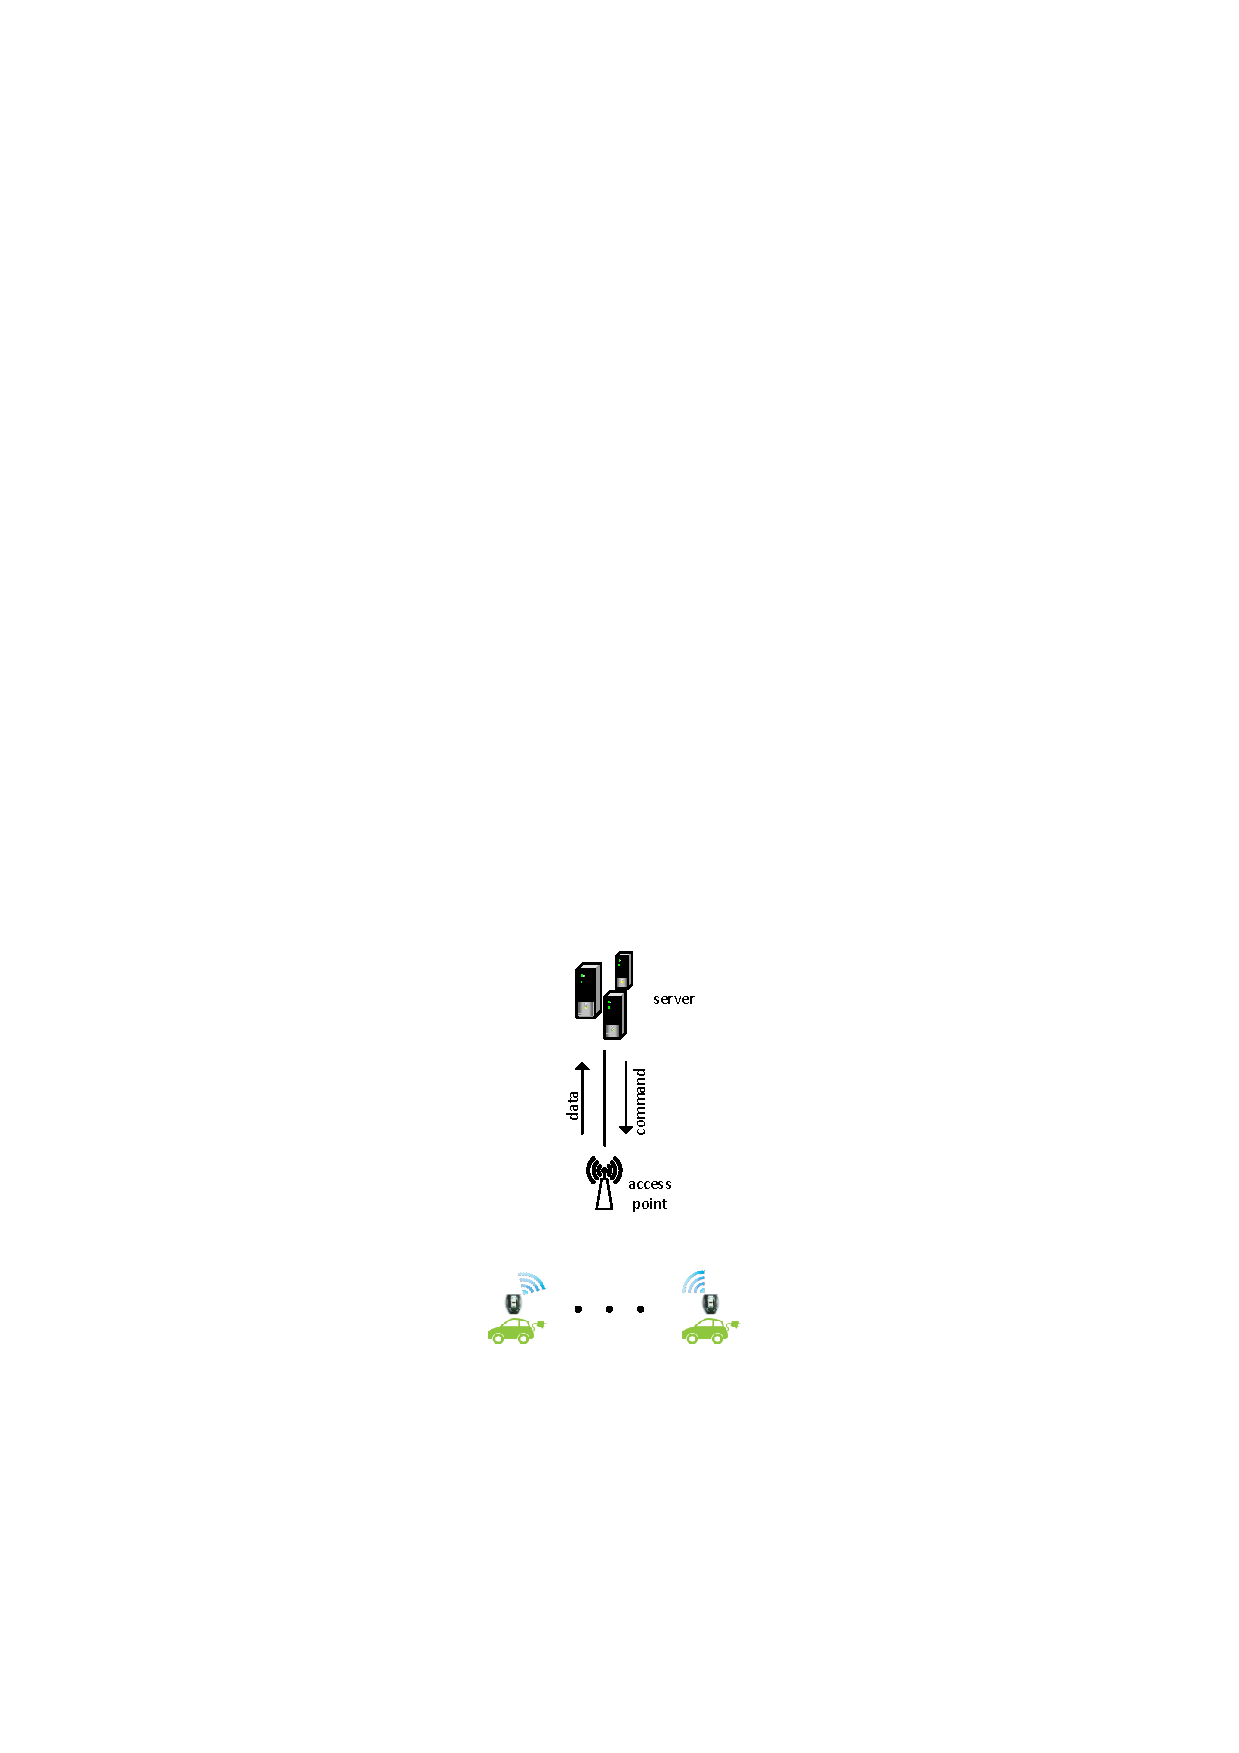
\includegraphics[width=\textwidth]{model-b.pdf}
						\caption{Communication model with server}
						\label{fig:model-b}
					\end{center}
				\end{subfigure}%  
\caption{System model \cite{lee2016adaptive}.} 
\label{fig:slackness1}
\endminipage
\end{figure}

		\begin{table} 
			\caption{Summary of key notations}\vspace{-3mm}
			\label{tbl:not}
			\begin{center}
				\begin{tabular}{|c L{6.5cm}|}
					\hline
					\textbf{Notation} & \textbf{Description} \\
					\hline \hline			
					$T$ & Number of time slots, indexed by $t$\\			
					$m$ & Number of CSs, indexed by $j$\\			
					$n$ & Number of EVs, indexed by $i$\\			
					\hline
					\hline
					$a_i$ & Arrival time of EV $i$\\
					$d_i$ & Departure time of EV $i$\\
					$D_i$ & Demand of EV $i$\\
					$v_i$ & Valuation of EV $i$ for receiving its demand $D_i$ \\
					$k_i$ & Maximum charging rate of EV $i$\\
					$h(i)$ & CS of EV $i$\\
					\hline
					\hline
					$q_j$ & Maximum $k_i$ among all EVs in CS $j$\\
					$p_j$ & Maximum aggregate charging rate in station $j$\\
					$p^\mathsf{total}$ & Maximum aggregate charging rate of all stations\\
					\hline
					\hline
					$y_i^t$ & \textbf{opt. variable}, The amount that EV $i$ is charged at $t$ \\
					\hline
				\end{tabular}
			\end{center}
		\end{table}
		\subsubsection{EVs}
		\label{sec:ev} There are $n$ EVs in the system, indexed by $i$.
		%, all available at time $t=1$ to be charged\footnote{This assumption is reasonable for the %official buildings where the starting hour of the working day is fixed for all the %employers. Extensions to the case with different arrival times for the EVs, is part of the %future work.}. 
		EV $i$ is represented by a charging profile $\langle a_i,d_i,v_i,D_i,k_i\rangle$ 
		indicating its arrival time, departure time, willingness to pay, charging demand, and maximum charging rate, respectively. 
		%(depends on physical properties of EVs battery) 
		More specifically, the charging of EV $i$ can be scheduled within its \emph{availability window}, $[a_i,d_i]$. The charging rate at each slot is bounded by $k_i$, a parameter that depends on the physical constraints of the \rev{battery and on-board charger}. It is assumed that the charging profile of each EV is feasible with respect to its maximum charging rate and a slackness parameter $s\geq 1$, which is the minimum ratio between the park time of the EV and its minimum charging time, i.e., ${D_i\leq k_i(d_i-a_i+1)/s}$. The slackness parameter is imposed to tune the flexibility of the charging scheduling. In extreme case $s=1$,  the flexibility is minimum and the flexibility improves as $s$ increases. 
%		Note  that  the slackness  parameter  can  impact  the  total  revenue  and  is  investigated  in  simulation  experiments  in Section~\ref{sec:simul}.
		We assume that EV owners select their CS, perhaps the nearest to them, and so the assignments are given to the problem. Define $h(i)$ as the CS of EV~$i$.
		Moreover, $q_j$ denotes the maximum $k_i$ among all EVs in CS $j$, i.e., $q_j=\max_{h(i)=j} k_i$. 
		\revv{Finally, $v_i$ is the willingness to pay of EV $i$ to receive its entire demand $D_i$ before the departure time $d_i$. Note that in resource-constrained EV scheduling in ACN, it is not feasible to fulfill the entire demand of all EVs, hence, the problem turns into a resource allocation one with the goal of maximizing the aggregate value (a.k.a. utility) obtained from the EVs. In this way, each user can announce its willingness to pay to get charged which is denoted by $v_i$ in the system model.}
		%We assume that there is no gain for the CS if EV $i$ is partially charged. 
		
		% where $P$ defined as $P:\xi\rightarrow  \mathcal{P}$. 
\subsubsection{Revenue Models\label{sec:irm}} We consider two revenue models: 
\textit{(i) Fractional revenue model}: In this model, the fractional charging is allowed, i.e., the revenue from each EV is proportional to the fraction of the demand that is fulfilled \cite{Xiang} (see Eq.~\eqref{Eq:partial_value}). We tackle this model in Section~\ref{sec:fractional}.
\textit{(ii) Integral revenue model}: \rev{In this model, EV $i$ pays $v_i$ if it is fully charged and zero otherwise, i.e., there is no partial revenue for partial charging. }
%In this model, when EV $i$ is received its demand entirely, the gain is $v_{i}$ and zero, otherwise, i.e., there is no partial revenue for fractional charging. 
This is the model that is considered in~\cite{WTang,Shroff2014}. We tackle this model in Section~\ref{sec:integral}.
		
		%The actual aggregated peak of all parking stations must not exceeds global peak constraint. 
		
		
			\begin{table*}[!t]
			\centering
	\vspace{-3mm}
			\caption{Proposed algorithms and their properties.}
			\label{tbl:algs}
			\begin{tabular}{ | l | c | c | c |c|}
				\hline
				\textbf{Algorithm} & \textbf{Revenue model} & \textbf{Type} & \textbf{Optimality} & \textbf{Complexity} \\ \hline\hline    
				\fcs& fractional& offline& Optimal & $O(n^2T+nT^2)$\\\hline 
				\ics& integral& offline& ${\Big( 1+\sum_{j=1}^m {\frac{p_j}{p_j-q_j}}.\frac{s}{s-1}\Big)}$-approximate & $O(nT\log T+n^2T)$ \\\hline 
				\focs & fractional& online& $2$-competitive & $O(n^2T)$\\\hline 
				\iocs& integral&  online& $b(1+\frac{p}{p-q}.\frac{s}{s-1})$-competitive, $(m=1)$ & $O(n^2T)$\\\hline
			\end{tabular}
		\end{table*}
		
		\subsection{Problem Formulation}
		\label{sec:problem}
	We formulate an optimization problem to schedule the charging of the EVs with the objective of maximizing total revenue obtained from charged EVs while respecting local and global peak constraints. 
		Note that each revenue model makes the underlying optimization problem fundamentally different. More specifically, the fractional charging model is a linear problem. 
		Integral revenue model, however, turns the underlying charging scheduling problem to a Mixed Integer Linear Program (MILP). The integer nature originates from the $0/1$-selection decision on EVs. 
%%%Recall that in integral revenue model the revenue is obtained given that the entire demand is fulfilled for the selected EV. 
		%We skip the explicit formulation of the problem under integral revenue model since it could be contemplated as the linear-relaxed version of the integral revenue model (for more explanation, we refer to the discussions in Section~\ref{sec:fractional}).
		We formulate Scheduling Problem for Adaptive charging Network (\MCSP) under fractional revenue model as follows: 
		\bse
		\bee
		\MCSP: \max  && \sum\nolimits_{i=1}^n \frac{v_{i}}{D_i}\sum\nolimits_{t=a_i}^{d_i} y_i^t \label{Pobjec} \nonumber\\
		\text{s.t.} &&\sum\nolimits_{t=a_i}^{d_i} y_i^t\leq D_i,\quad\quad\forall i, \label{ConstPartial} \\
		&&  \sum\nolimits_{i=1}^n y_i^t\leq p^\mathsf{total} ,\quad\quad\forall t,\label{ConstTotal} \\
		&&\sum\nolimits_{i:h(i)=j} y_i^t\leq p_j ,\quad\quad\forall t,j,\label{ConstLocal}\\
		&& y_i^t  \leq \frac{k_i}{D_i}\sum\nolimits_{t^\prime=a_i}^{d_i} y_i^{t^\prime}, \quad\forall i,t,\label{ConstSpeed}\\
%		&& \rev{y_i^t=0,\forall t\in\{t':t'>d_i \vee t'<a_i\}}, \\
		\text{vars.} && y_i^t \geq 0, \quad\quad\forall i, t,\label{ConstPositive}\nonumber
		%&& s_v(t), \quad \forall v,t
		\eee
		\ese
		where $y_i^t$ is the amount that EV $i$ is charged at slot $t$. Constraint (\ref{ConstPartial}) ensures that the aggregate amount received by EV $i$ is at most the demand $D_i$. 
%		Note that under integral revenue model, when we design our algorithm, we do not allow partial charging. 
The global and local peak constraints are represented by constraints (\ref{ConstTotal}) and (\ref{ConstLocal}), respectively. 
		
		\revv{The constraint~\eqref{ConstSpeed} enforces the maximum charging rate of EVs. The straightforward way to express this constraint is to simply state that at each time slot $t$, the charging rate of EV $i$ should be less than or equal to its maximum charging rate, i.e., $y_i^t\leq k_i, \forall i,t$. 
		However, for the sake of effective algorithm design for integral model and reducing the integrality gap of the relaxed linear problem, this constraint is strengthened in the form of Eq.~\eqref{ConstSpeed}. 
		Note that in case that the aggregated charging of EV $i$ during its availability window is equal to its demand, i.e., $\sum_{t^\prime=a_i}^{d_i} y_i^{t^\prime}= D_i$, Eq.~\eqref{ConstSpeed} reduces to the simple form of $y_i^t\leq k_i$.  
		This is a natural way in approximation algorithm design to improve the performance of the algorithms under linear-relaxation based design~\cite{Carr}. } 
	
	
The \MCSP is an extension of formulated problem in \cite{Jain} where a job scheduling problem in cloud applications is studied. It turns out that the resource allocation problem in cloud systems and the EV charging scheduling problem in a \emph{single station} share similar structure. Indeed, each charging profile in our scheduling problem can be seen as a job in cloud system with a deadline, value, and CPU demand. The \MCSP, however, comes with an additional constraint~\eqref{ConstTotal}, which makes it different from the problem in \cite{Jain}, such that the existing solution \revv{will not} work in the new setting. More importantly, this paper studies both offline and online solutions for the problem in both fractional and integral settings, while \cite{Jain} tackles only the offline integral model.  
		
%(ii) Our solution design and analysis for integral revenue model is based on linear-relaxation primal-dual framework~\cite{Jain}. Therefore, in Section \ref{sec:integral} for integral revenue model, we rely on the \MCSP for the analysis of the proposed algorithms and skip to explicitly formulate the original MILP problem.



%		Also, we cover the fractional revenue model and provide theoretical bounds for the proposed algorithms.
		
%In the next two sections, we devise several algorithms to solve the \MCSP under the two revenue models (integral and fractional) and for both offline and online scenarios. 
		\section{Fractional Revenue Model}
		\label{sec:fractional}

%\subsection{Overview of Fractional Revenue Model}
%\label{sec:frac.overview}				
		%In the previous section, we devised an approximation algorithm for the integral revenue model in which it is assumed that the obtained revenue is zero if the allocated resource is less than the demand. Although this assumption is reasonable in some scenarios, 
%To develop a solution for the \MCSP, we first consider fractional revenue model.
%However, algorithms for integral revenue model cannot achieve the same performance as the algorithms of this section i.e., \fcs and \focs. 

In the fractional model, the revenue of the CS from EV $i$ is directly proportional to the amount of resource that the EV is received, i.e.,
		\begin{equation}
			v_i^{\mathsf{f}}=\frac{\sum_t y_i^t}{D_i}v_i,
			\label{Eq:partial_value}
		\end{equation}
		where $v_i$ is the gain, if the entire demand $D_i$ is fulfilled and $v_i^{\mathsf{f}}$ is the fractional gain.  

%Under fractional revenue model and without the binary variable of selecting EVs, the underlying problem turns into a linear one. 
We propose a simple algorithm, called \fcs, with low computational complexity \rev{ of $O(n^2T+nT^2)$} for the fractional model that finds the optimal solution in offline setting. Note that even though linear programs can be solved in polynomial time in general, the complexity of our proposed algorithm is much lower than the general linear program algorithms. Moreover, our proposed offline algorithm applies a valley-filling strategy to reduce the peak. 
%The details of the proposed algorithm \fcs is given in~\cite{alinia2017online}. In the following, the online $2$-competitive algorithm is designed, where no exact information or stochastic modeling of future inputs of the problem is available. 
A summary of proposed algorithms with their complexity and assumptions is given in Table \ref{tbl:algs}.		

\revv{
\subsection{Optimal Offline Design}
\label{sec:fopt}				
We refer the proposed algorithm as the \fcs and summarize it as Algorithm~\ref{alg:optimal-off}.
The \fcs works in two phases. In the first phase (Section~\ref{sec:ph1}), the algorithm decides on the amount of resource to be allocated to each EV within its availability window and reserves resources accordingly. In this phase, the details of allocation is not known. The actual resource allocation is done in the second phase (Section~\ref{sec:ph2}) by setting variables $y_i^t$.

Before discussing the details of the algorithm, we give a definitions and introduce some notations to facilitate our algorithm design.

\begin{defi}
	Time interval $[\delta,\delta']$ is a ``super interval'' for interval $[t,t']$ if $1\leq \delta\leq t \text{~AND~} t' \leq \delta'\leq T$.
	Moreover, $\mathcal{I}_{t,t'}$ is the set of all super intervals of interval $I_{t,t'}$ i.e., ${\mathcal{I}_{t,t'}=\{[\delta,\delta']: 1\leq \delta\leq t \text{~AND~} t'\leq \delta'\leq T\}}$.
\end{defi}

%		For example, $\mathcal{I}_{1,1}=\{I_{1,1},I_{1,2},I_{1,3},\dots ,I_{1,T}\}$. 
The number of super intervals of an interval is at most $T^2$ and at least one (for interval $[1,T]$). 

Let $R_i$ be the amount of resource that is reserved for EV $i$ by the \fcs and $I_{t,t'}$ as time interval $[t,t']$.
% with $t,t'\in\{1,\dots ,T\}$ which includes time slots $t,t+1,\dots ,t'$. 
Then, assuming that charging demands are sorted in non-increasing order of their unit values, $A^i_j(t,t')$ is the aggregate residual resource in interval $I_{t,t'}$ at station $j$ assuming that the reservation for EVs $1$ to $i$ is accomplished. We now explain in detail each phase of the algorithm. 


\subsubsection{Phase I-Reservation\label{sec:ph1}} In Line~\ref{algline:sort1}, the EVs are sorted in a non-increasing order of their unit values.  
%		i.e., ${v_1\slash D_1\geq v_2\slash D_2\geq\dots \geq v_n\slash D_n}$. 
In Line~\ref{algline:setR}, the \fcs processes demand of EV $i$, picked from top of the ordered list, and sets $R_i$ as the amount to be reserved for EV $i$ which will be allocated in Phase II. In Line~\ref{algline:seta}, the residual resource of all intervals in set $\mathcal{I}_{a_i,d_i}$ decreases by $R_i$ and EV $i$ is added to the set of selected EVs.


\begin{algorithm}[t]%\small%1
	%\footnotesize
	\revv{
	\caption{\fcs}
	\label{alg:optimal-off}
	\DontPrintSemicolon 
	\KwIn{$n$ EVs with their profile, local and global peak constraints $p_j, j=1,\dots ,m$ and $p^\mathsf{total}$ }
	
	\KwOut{Optimal scheduling under fractional model}
	\BlankLine
	
	Sort charging requests in non-increasing order of their unit values, i.e., $\frac{v_1}{D_1}\geq \frac{v_2}{D_2}\geq\dots \geq \frac{v_n}{D_n}$\label{algline:sort1}
	
	%	\slash\slash\textit{\texttt{Use sorted list to process demands}}
	
	$\mathcal{L}\leftarrow \emptyset$ 	
	
	\slash\slash\textit{\texttt{Phase I}}
	
	
	\For{$i=1,\ldots, n$}{
		%\slash\slash\textit{\texttt{update demand and value}}
		
		$R_i \leftarrow \min\{D_i, \min\limits_{t,t'} A^{i-1}_{h(i)}(t,t'), \forall t,t': I_{t,t'}\in\mathcal{I}_{a_i,d_i}\}$\label{algline:setR}
		
		\If{$R_i>0$}{
			$A^{i}_{h(i)}(t,t')\leftarrow A^{i-1}_{h(i)}(t,t')-R_i, \forall t,t': [t,t']\in\mathcal{I}_{a_i,d_i}$ \label{algline:seta}\\
			$\mathcal{L}\leftarrow \mathcal{L}\cup{i}$
	}}
	\slash\slash\textit{\texttt{Phase II}}
	
	Sort EVs in $\mathcal{L}$ in increasing order of their charging flexibility i.e., $\frac{(d_i-a_i+1)k_i}{D_i}, i\in \mathcal{L}$. 
	
	%	Let $i$ be the index of $i^{th}$ EV in list $\mathcal{L}$
	
	\For{$i=1,\ldots, |\mathcal{L}|$}{
		
		Pick EV $i$ from the sorted list $\mathcal{L}$. 
		
		$\emph{feasible}\leftarrow \big(\sum_{t=a_i}^{d_i}\min\{k_i,A^{i-1}_{h(i)}(t,t)\}\big) - R_i$
		
		\If{feasible $<0$}{
			Re-allocate previously allocated EVs such that $\emph{feasible}\geq 0$
		}
		Arbitrarily allocate $R_i$ to EV $i$ in its availability window\label{algline:fcsallocate}	
	}}
\end{algorithm}



\begin{lem}
	Provided that for EV $i$ we have 
	\bee
	\label{eq:ri}
	R_i\leq\min\left\{D_i, \min_{t,t'} A^{i-1}_j(t,t'), \forall t,t': I_{t,t'}\in\mathcal{I}_{a_i,d_i}\right\}
	\eee
	 with a dummy $A^0_j(t,t')$ defined as
$A^0_j(t,t')=(t'-t+1)\times\min \{p^\mathsf{total},p_{j}\},$
	then there is a feasible allocation to allocate $R_i$ to EV $i$ in its availability window $[a_i,d_i]$. 
	\label{thm:R_feasible}
\end{lem}


In Lemma \ref{thm:R_feasible}, $A^0_j(t,t')$ indicates the available resource when no charging request is processed in $I_{t,t'}$. 
In Eq.~\eqref{eq:ri}, the second term, i.e., $\min_{t,t'} A^{i-1}_{j}(t,t')$, indicates the minimum remaining resource in all super intervals of interval $I_{a_i,d_i}$. For $i\geq 1$, $A^i_j(a_i,d_i)$ is defined as follows:

\begin{equation*}
A^i_j(a_i,d_i)=\begin{cases}
A^{i-1}_j(a_i,d_i)-R_i & j=h(i),\\
A^{i-1}_j(a_i,d_i) & j\neq h(i).
\end{cases} 
\end{equation*}

The optimal value of $R_i, i=1,\dots ,n$ is set according to the following lemma:

\begin{lem}
	Given $n$ EVs sorted in a non-increasing order of the unit values, ${v_1\slash D_1\geq v_2\slash D_2\geq\dots \geq v_n\slash D_n}$, and the value of $R_i$, where $R_i$ is set after $R_{i-1}, i=2,\dots ,n$ by Eq.~\eqref{eq:ri}, then, 
	$$R_i = \min\left\{D_i, \min_{t,t'} A^{i-1}_{h(i)}(t,t'), \forall t,t':I_{t,t'}\in\mathcal{I}_{a_i,d_i}\right\},\forall i,$$
	is the optimal value for $R_i$. 
	\label{thm:R_star}
\end{lem}

\subsubsection{Phase II- Allocation\label{sec:ph2}} Lemma~\ref{thm:R_feasible} shows that there is a feasible scheduling to allocate the reserved resources.
However, despite its feasibility, it is not straightforward to find such \revv{a schedule}. For example, assume that for EV $i$, $R_i=10$ and $k_i=4$. It is possible that all available resources are concentrated in a single time slot but EV $i$ cannot use more than $4$ kWh of it. In this situation, the previously allocated resources in interval $I_{a_i,d_i}$ should be re-allocated such that the concentrated resources are \emph{dispersed} and we have $\sum_{t=a_i}^{d_i}\sigma_t \geq R_i$ where $\sigma_t =\min\{k_i,A^{i-1}_{h(i)}(t,t)\}$ is the maximum resource that can be allocated to EV $i$ at time slot $t$. Since the total amount of allocated resource does not change in the interval, such dispersion is possible and can be done by a simple algorithm in which allocates $\min\{k_i,A^{i-1}_{h(i)}(t,t)\}$ starting from time slot $t=a_i$ until $R_i$ units is allocated. To further reduce the peak of the system, we will develop \sa\ algorithm (See Section \ref{sec:integral}) which acts more intelligent so that Line \ref{algline:fcsallocate} of the \fcs can be replaced by ``Run \sa$(i,R_i)$''.



\begin{thm}
	\label{cor:1}
	\fcs is an optimal solution under fractional revenue model.
\end{thm}

The following theorem characterizes the complexity of \fcs.

\begin{thm}
	\label{thm:complexity}
	The time complexity of \fcs algorithm is $O(n^2T+nT^2)$ where $n$ is the number of EVs and $T$ is number of time slots.
\end{thm}
}

\vspace{-4mm}
\subsection{Online Scenario}
\label{sec:fonline}
In this section, we devise an algorithm for the scenario that EVs arrive in online fashion. The scheduling decisions at each time slot are made given the information of available EVs and neither exact values nor stochastic modeling of future arrivals is available. Our goal is to obtain a \emph{competitive ratio} for the online algorithm. A scheduling algorithm $\mathcal{A}$ is $c$-competitive for $c\geq 1$ if the revenue obtained by the optimal offline algorithm is at most $c$ times the algorithm $\mathcal{A}$'s revenue for any input sequence~\cite{borodin2005online}.

The proposed online algorithm for the fractional model, referred to as \focs, is listed as Algorithm~\ref{alg:focs}. The \focs is a simple yet efficient algorithm that always selects EVs with highest unit value to allocate as follows. First, the algorithm sorts the available EVs at each time slot~$t$ based on their unit value (Line~\ref{algline:sort}). \revv{In this step, the algorithm breaks ties based on EVs' deadline i.e., if two EVs have the same unit value, then the one with earliest deadline comes first in the sorted list.} Next, the \focs selects one EV at a time from the sorted list to allocate with maximum charging rate considering the EV's remaining demand, maximum charging rate, and peak constraints (Lines~\ref{algline:focsfor}-\ref{algline:focssety}). The allocation is continued until all resources are allocated or there is no more EV that could be allocated. 
%For unselected EVs, the value of $y_i^t$ will be $0$ in Line \ref{algline:focssety} of the algorithm. 
The time complexity of the \focs is $O(n^2T)$, determined by cost of its ``\textbf{for}'' loop multiplied by total number of times that the algorithm needs to be run.
% i.e., $T$. 

\vspace{-4mm}
\begin{algorithm}%\small%1
\footnotesize
\caption{\focs: $\forall t\in \{1,2,\dots ,T\}$}
\label{alg:focs}
\DontPrintSemicolon 
%\KwIn{Available EVs at time slot $t$, number of CSs $m$, local peak constraint $p_j, j=1,\dots ,m$, global peak constraint $p^{\textrm{total}}$}

%\KwOut{A feasible charging scheduling}

%$\backslash\backslash\texttt{Initialize:}$

\BlankLine

$\mathcal{M}^t\leftarrow$ The set of available EVs that not received their entire demand by $t$ 

Sort EVs in set $\mathcal{M}^t$ indexed by $i=1,\dots ,|\mathcal{M}^t|$: $v_1/D_1\geq v_2/D_2\geq\dots\geq v_{|\mathcal{M}^t|}/D_{|\mathcal{M}^t|},$  \revv{where ties are broken based on users' deadline (giving priority to the users with earliest deadline) }\label{algline:sort}

\For{$i=1,\ldots,|\mathcal{M}^t|\label{algline:focsfor}$}{

$y_i^t\leftarrow \min\{k_i,D_i-\sum_{\tau=a_i}^{t}y_i^{\tau},p_{h(i)}-\sum_{i':h(i')=h(i)}y_{i'}^t,p^{\textrm{total}}-\sum_{i'}y_{i'}^t\}$ \label{algline:focssety}

}

\end{algorithm}
Despite the simplicity of \focs which makes it easy to implement, its performance is sound and within a constant factor of the offline optimum. We now proceed to analyze the performance of the \focs by first giving some preliminaries. 

Fix an optimal scheduling and let $\mathcal{S}_{\focs,t}$ and $\mathcal{S}_{\opt,t}$ be the sets of EVs selected by the \focs and optimal solution at time slot $t$, respectively. Let $y_{i}^t$ and $z_{i}^t$ be the charging rate of EV $i$ set by \focs and \opt, respectively. We define $\Delta_{i}^t$ as follows:
\begin{equation}
\label{eq:delta}
\Delta_{i}^t =
     \begin{cases}
       \min\{z_{i}^t-y_{i}^t,r_{i,t}\} &\quad i\in\mathcal{S}_{\opt,t},z_{i}^t>y_{i}^t, \\
       0& \quad\text{otherwise},  \\
     \end{cases}
\end{equation}
where $r_{i,t}$ is the remaining demand of EV $i$ by the end of time slot $t$. $\Delta_{i}^t>0$ indicates that the optimal algorithm allocated $\Delta_{i}^t$ units more resources to EV $i$ than the \focs by time slot $t$ that could be \emph{feasibly} allocated by \focs to the EV $i$. If for any EV $i\in\mathcal{S}_{\opt,t}$ and time slot $t\in\mathcal{T}$ we have $y_{i}^t=z_{i}^t$, i.e., $\Delta_{i}^t=0$, then the \focs is obviously optimal because it gains whatever the optimal solution gains. \rev{We define \textit{loss} of the \focs imposed by EV $i$ as follows:
\begin{equation}
\label{lBj0}
l_{i,t}=\Delta_{i}^t\frac{v_i}{D_i},
\end{equation}

Note that the loss always takes a non-negative value as $\Delta_i^t\geq 0$.} When \focs sets charging rate of an EV less than its rate in the optimal solution, it gains $\Delta_{i}^t v_i/D_i$ less than the optimal solution from that EV. An upper bound for the distance between the optimal objective value (denote by \opt) and the revenue of the \focs (denote by \alg) is summation of the losses over all time slots and all EVs, i.e., 
\begin{equation}
\label{eq:optdist}
\opt-\alg\leq \sum_{t=1}^T\sum_{i\in\mathcal{S}_{\opt,t}} l_{i,t}.
\end{equation}

%Notice that it is possible that an algorithm does not choose any selected EV by a particular optimal solution but still provide an optimal or near-optimal solution as there can be multiple optimal solutions. In particular, $\mathcal{S}_{\focs,t}\cap \mathcal{S}_{\opt,t}=\emptyset, \forall t$ cannot lead to any conclusion on the competitive ratio of the \focs. 
In addition to the amount of loss, the gain of the algorithm from charging alternative EVs should also be taken into account in comparison between \opt and \alg. 

Let $i\in\mathcal{S}_{\opt,t}$, $i\notin\mathcal{S}_{\alg,t}$ and $g_{i,t}$ be the gain that the \focs obtains from charging another EV instead of $i$ at time slot $t$. We are going to show that in the \focs, for each EV $i$ with $l_{i,t}>0$ there must be another EV (denote by $i'$) where $y_{i'}^t\geq \Delta_i^t$ and $\frac{v_{i'}}{D_{i'}}\geq \frac{v_i}{D_i}$ which means in resource allocation phase for EV $i$, the \focs allocated the difference $\Delta_i^t$ to another EV with the same or higher unit value. This can be proved by considering the fact that (i) the selected EVs have higher unit values than the unselected EVs, and (ii) the charging rate of the selected EVs are set to the maximum feasible value. Moreover, the \focs is \emph{``work-conserving''} i.e., it does not let any resource remain unused if there are some EVs that can use it. 

Let $g_{i,t}$ denote the gain that \focs obtains from allocating the same amount of resource that optimal algorithm allocated to EV $i$ (with size $z_i^t$) to another EV(s).
If $\Delta_{i}^t=0$, the loss is zero. If $\Delta_{i}^t>0$, then by the charging strategy that the \focs uses we can conclude that (i) $i$ is not finished by the \focs, and (ii)
\rev{no more resources from station $p_{h(i)}$ can be feasibly allocated,} otherwise, the \focs could allocate more resources to EV $i$. Therefore, the $\Delta_{i}^t$ units of the resource \rev{are} allocated to one or multiple other EVs (denote them by set $\mathcal{J}_i^t$) by the \focs. Moreover, it must hold that all the EVs in set $\mathcal{J}_i^t$ have a unit value equal to or higher than $v_i/D_i$ which yields $g_{i,t}\geq l_{i,t}$, otherwise, the \focs should not prefer the EVs in $\mathcal{J}_i^t$ to $i$. \rev{Since the result holds for any arbitrarily EV $i$, we can get the following:}

\begin{equation}
\label{eq:lg}
\sum_{i=1}^n\sum_{t=1}^Tl_{i,t}\leq\sum_{i=1}^n\sum_{t=1}^Tg_{i,t}.
\end{equation}

Moreover, the total gain of \focs, i.e., \alg, is equal to sum of its gains from each single EV:
\begin{equation}
\label{eq:ALG}
\rev{\alg= \sum_{i=1}^n\sum_{t=1}^Tg_{i,t}.}
\end{equation}

With the above discussion and using Eqs. (\ref{eq:optdist}), (\ref{eq:lg}) and (\ref{eq:ALG}) we are able to derive a competitive ratio of $2$ for the \focs. 

\begin{thm}
	\label{thm:focscompetitive}
	The \focs is $2$-competitive.
\end{thm}



\emph{Remarks:} When there is only one CS and EVs have no limit on their charging rate, the \focs is identical to the \textsc{FirstFit} algorithm ~\cite{firstfit} which is known to be $2$-competitive for classic job scheduling problem. However, the charging rate limitation is crucial for EV charging problem. Moreover, \cite{firstfit} uses \revv{a} ``charging argument'' to prove the competitive ratio of the proposed algorithm which cannot be directly applied to our problem. Thus, the \focs extends the \textsc{FirstFit} and makes it practical for the EV charging scenario. Moreover, the proof technique used for the competitive analysis of the \focs is fundamentally different from the one used in \cite{firstfit}. 
%%%Finally, in~\cite{Robu} an online $2$-competitive algorithm for EVs with partial charging is proposed. The competitive ratio obtained assuming that charging of EVs is instantly reversible at departure times. This assumption is not practical in reality since similar to charging phase, there is a discharging rate constraint for EVs.

%\begin{thm}
%\label{thm:focscomplexity}
%
%The time complexity of \focs is $O(nT\log n)$.
%\end{thm}
		\section{Integral Revenue Model}
		\label{sec:integral}
%
%		\subsection{Overview of Integral Revenue Model}
%		\label{sec:intoverview}
		The MILP form of the \MCSP in integral model is a generalized form of the $0/1$-knapsack problem which is a well-known NP-hard problem. \rev{To give an intuition, consider the scheduling problem in a single time slot (i.e, $T=1$). Then, allocating power resources to the EVs is equivalent to allocating the capacity of knapsack to the items. }	
		In Section~\ref{subsec:icsalgorithm}, we propose a fast polynomial time offline approximation algorithm for the integral problem. In Section~\ref{sec:onlineint}, we extend the result and propose an online algorithm for the integral model.
%		, where the EVs arrive in slot-by-slot fashion, and the scheduler has no information of the future arrivals. 
		
%The problem is even more challenging when the uncertainty in EVs' arrival is taken into account. At each time slot, the scheduler has no information of unit values of the future charging profiles. Therefore, the scheduler cannot make sure about the efficiency of its current charging decision.
%It can be shown that when there is no assumption on the charging profiles of EVs (including the value of slackness parameter) and the charging decision , no online algorithm can provide a performance guarantee meaning that in the worst case, the ratio of the optimal objective value to the one obtained by the online algorithm can be arbitrary small. In fact, when the online algorithm selects
		
		\subsection{Offline Scenario}   
		\label{subsec:icsalgorithm}
		We design our offline scheduling algorithm under integral model referred to as \ics, to solve the \MCSP approximately. 
%		Our algorithm design is inspired by the basic algorithm proposed in \cite{Jain}. The algorithm in \cite{Jain} works for a single CS where arrival time of all EVs are the same and there is no global peak constraint. 
Since the performance analysis of the proposed algorithm relies on a dual fitting method and utilizes weak duality property, \revv{we first need to construct the dual problem of \MCSP. Toward this, we introduce variables $\alpha, \beta, \gamma$ and $\pi$. Generally, in primal-dual approximation algorithm design, each constraint (resp. variable) in primal (resp. dual) problem is associated with a variable (resp. constraint) in dual (resp. primal) problem. In our case, constraints (\ref{ConstPartial}) (\ref{ConstTotal}), (\ref{ConstLocal}) and (\ref{ConstSpeed}) in the \MCSP are respectively associated with dual variables $\alpha, \beta, \gamma$ and $\pi$ (for more details see \cite{approx}). The dual problem is formulated as follows:}
		\bse
		\bee
		\min &&\sum_{i=1}^n D_i\alpha _i + \sum_{j=1}^m \sum_{t=1}^T p_j\beta (t)+\sum_{t=1}^T p^\mathsf{total}\gamma (t)\nonumber\\ 
		\textrm{s.t.} && \alpha _i+\beta (t) +\gamma _i + \pi (t)- \frac{k_i}{D_i}\sum_{t'=a_i}^{d_i} \pi _i(t^\prime) \geq \frac{v_{i}}{D_i},\label{ConstDcover} \nonumber\\
		&& \quad\quad\quad\quad\quad\quad\quad\quad\quad\quad\forall i, t\in [a_i, d_i],\\
		\textrm{vars.}&&\alpha _i, \beta _i, \gamma,  \pi _i(t)\geq 0,\quad\quad\forall i,t. \nonumber
		\eee
		\ese

		
		%%%In this section, we explain \ics in details and then in Section~\ref{subsec:analysis}, we analyze approximation factor of the algorithm. The \ics algorithm is listed as Algorithm~1.
		
		\subsubsection{Explanation of the Main Algorithm} 
		\label{sec:icsexplanation}
		Our algorithm design is inspired by the basic algorithm proposed in \cite{Jain}. \revv{The algorithm in~\cite{Jain}, however, works for a single CS where arrival time of all EVs are the same and there is no global peak constraint.}
		The \ics algorithm (listed as Algorithm \ref{alg:ics}) works in two phases. In the first phase it sorts the charging requests based on their unit values in a non-increasing order. Then, it selects most valuable demand. If the remaining resource is enough to cover the \emph{entire} demand of the EV, it is admitted to receive the demand (Lines~$6$-$7$). 
%		When \ics processes EV $i$, the algorithm checks for the feasibility of allocating $D_i$ units of the resource within its availability window $[a_i,d_i]$ without violating the constraints related to the maximum charging rate $k_i$, local and global peaks (Lines~$6$-$8$).	 	
		
		\emph{Scheduling of the Selected EV:} \revv{If the feasibility check passed (Line 6 in Algorithm 3)}, \ics calls sub-procedure \sa\ to allocate required resources in interval $[a_i,d_i]$. Then, $\alpha _i$ is set to $v_i\slash D_i$ in order to cover dual constraint in Eq.~\eqref{ConstDcover} (Lines~$7$-$8$). 
		
		In \sa, 
		%%%When EV $i$ is selected to get charged, \sa\ is called for the charging scheduling. 
		let us define $W(t,h(i))=\sum_{i': h(i')=h(i)} y_{i'}^t$ as total workload at time slot $t$ in CS $h(i)$ and $\bar{W}(t,h(i))$ as total available load to allocate at time slot $t$ for CS $h(i)$. We always have ${\bar{W}(t,h(i))+W(t,h(i))=p_{h(i)},  \forall t, i}$. For scheduling, \sa\ applies two main policies: 1) \emph{valley-filling} and, 2) \emph{right-to-left allocation}. \revv{With valley-filling, the slots with more available resources are preferred which helps to reduce the peak of the system.} %%%It also can be seen as a smoothing method which tries to reduce the variance of the allocated resources at different slots. 
%				The simulation results in Section \ref{sec:simul} will confirm this claim. 
				Right-to-left allocation is used when two or more time slots are equal in terms of their remaining resources. 
%				When this policy applies on scheduling of EV~$i$, any EV~$i'$ with $i'>i$ and $d_{i'}<d_i$ has more chance to get charged since the algorithm tends to charge EV $i$ in interval $[d_{i'}+1,d_i]$ (i.e., right hand part of the EV's availability window) and keeps resources in $[a_{i'},d_{i'}]$ for EV $i'$. 
A ranking based approach is used to apply the aforementioned policies. 
		To charge  EV $i$, \sa\ ranks time slots in interval $[a_i,d_i]$. Then, charging is done by allocating resources from the higher ranked time slot to lowest one. The rank of a time slot $t$ is calculated based on remaining resources in the time slot (valley-filling) and value of $t$ (right-to-left allocation). 
		
		\vspace{-3mm}
		\begin{algorithm}%\small%1
			\footnotesize
			\caption{\ics}
			\label{alg:ics}
			\DontPrintSemicolon 
%			\KwIn{$n$ EVs with $a_i, d_i, v_i, D_i,$ and $k_i$ associated with each EV $i$, $m$ CSs, local and global peak constraints $p_j, j=1,\dots ,m$, and $p^\mathsf{total}$}
			
%			\KwOut{A feasible scheduling of EVs}
			\BlankLine
			%\begin{algorithmic}
			
			%\slash\slash\textit{\texttt{Initialization}}
			\textbf{initialize}: $y\leftarrow 0, \alpha\leftarrow 0, \beta\leftarrow 0, \gamma\leftarrow 0, \pi\leftarrow 0$
			
			Sort charging requests in non-decreasing order of their unit values: $v_1/D_1 \geq v_2/D_2\geq\dots \geq v_n/D_n$
%			$\frac{v_1}{D_1} \geq \frac{v_2}{D_2}\geq\dots \geq \frac{v_n}{D_n}$
%			\slash\slash\textit{\texttt{Use sorted list to process demands}}
			
			\For{(i=1\dots n)}{				

				\For{$t=a_i\dots d_i$}{
					$\sigma_t\leftarrow  \min\Big\{p_{h(i)}-\sum_{i':h(i')=h(i)}y_{i'}(t),$ \newline $\qquad p^\mathsf{total}-\sum_{i'=1}^n y_{i'}^t,k_i\Big\}$
					
				}
				
				
%				\slash\slash\textit{\texttt{if enough resources remain for EV $i$}}

				\If{$D_i\leq\sum_{t=a_i}^{d_i}\sigma_t$}
				{
					\sa($i,D_i$)\\
					$\alpha _i\leftarrow v_i/ D_i$
				}
				\Else {
					\If{$(\beta (d_i)=0)$}{
						\bc($i$)}
				}
			}
			
			\For{(i=1\dots n)}{ 
				\If {EV $i$ is not selected}{
					\rc($i$);
				}
			}
			%\end{algorithmic}
		\end{algorithm}
	
		
\emph{Dual Feasibility of the Non-selected EVs:} If there is not enough resources to fully charge EV $i$, i.e.,  $D_i>\sum_{t=a_i}^{d_i}\sigma_t$, the EV cannot be selected. However, we still need to satisfy constraint~\eqref{ConstDcover} in dual problem which is done by calling \bc($i$). To cover the constraint~\eqref{ConstDcover} for EV $i$, sum of dual variables for all $t\in [a_i ,d_i]$ should be greater than or equal to ${v_i \slash D_i}$. \bc($i$) sets $\beta (t)$ to ${v_i \slash D_i}$ for all time slots $t$ in interval $[t_\mathsf{cov}, R(d_i)]$ (Lines $3$-$4$ of Algorithm~\ref{alg:betacover}). Observe that  ${\beta (t^\prime)\geq v_i \slash D_i,\forall t^\prime< t_\mathsf{cov}}$ (with $ t_\mathsf{cov}>1$) considering that the demands are sorted in a non-increasing order of the unit-values and $\beta (t')$ is already set to ${v_{i'} \slash D_{i'}}$ when processing the earlier charging demand of EV $i'$ which is not selected. Hence, ${v_{i'}\slash  D_{i'}\geq v_i \slash D_i}$, thereby ${\beta (t)\geq v_i \slash D_i,}$ and the dual constraint in~\eqref{ConstDcover} is satisfied.		
		Lines $1$-$4$ of \bc\ is enough to cover the dual constraint. However, the algorithm continues in Lines $5$-$8$ by setting a variable $\Phi_{i'}(t)$ for time slots $t=1,\dots ,R(d_i)$ to a value dependent to amount of the resource that a selected EV $i'$ received at slot $t$. $\Phi_{i'}(t)$ will be used in approximation analysis of the main algorithm and has no effect on the scheduling of EVs. 
		%We borrowed algorithm \bc($i$) from \cite{Jain} and adjusted it for multiple station mode.		
		\vspace{-3mm}
		\begin{algorithm}%\small%1
			\footnotesize
			\caption{\sa($i,D_i$)}
			\label{SmartAllocate}
			\DontPrintSemicolon 
			\KwIn{EV $i$ to receive $D_i$ from CS $h(i)$}
			
			Rank time slots in interval $[a_i,d_i]$ such that for any $t_1$ and $t_2$:
			$\mathsf{rank}(t_1)> \mathsf{rank}(t_2)$ iff $\bar{W}(t_1,h(i))>\bar{W}(t_2,h(i))$ OR $\bar{W}(t_1,h(i))==\bar{W}(t_2,h(i)) \wedge t_1>t_2$ 
			
			\While {$\sum_{t'=a_i}^{d_i}y_i^{t'}\neq D_i$}{
				
				Select time slot $t$ with highest rank which is not selected before
				
				Allocate $\min \left\{k_i,\bar{W}(t,h(i)),D_i-\sum_{\tau=a_i}^{t}y_i^{\tau},p^{\textrm{total}}-\sum_{i'}y_{i'}^t\right\}$ to EV $i$ at $t$
				
			}
		\end{algorithm}	
		\vspace{-7mm}	
		\begin{algorithm}%\small%1
			\footnotesize
			\caption{\bc($i$)}
			\label{alg:betacover}
			\DontPrintSemicolon 
			%\KwIn{EV $i$ which is not selected to charge}
			
			\BlankLine
			
			$t_\mathsf{cov}\leftarrow \min \{t: \beta (t)=0\}$
			
			$R(d_i)=\max \{t\geq d_i : \forall t^\prime\in (d_i,t], \bar{W}(t^\prime)<q_{h(i)} \}$
			
			\For{$(t=t_\mathsf{cov}\dots R(d_i))$}{
				$\beta (t)\leftarrow v_i/D_i$
			}
			
			\For{$(t=1\dots R(d_i))$}{
				\For{$(i'=1\dots n))$}{	
					\If{$y_{i'}^t>0 \wedge \Phi_{i'}(t)=0$}{
						$\Phi_{i'}(t)\leftarrow\big[ \frac{p_{h(i)}}{p_{h(i)}- k_i}\frac{s}{s-1}\big] .\frac{v_i}	{D_i}y_{i'}^t$
					}
				}
			}
		\end{algorithm}
		\vspace{-7mm}
		\begin{algorithm}%\small%1
			\footnotesize		
			\caption{\rc($i$)}
			\label{Replace}
			\DontPrintSemicolon 
%			\KwIn{EV $i$}
%			\KwOut{Updated schedule}
			
			$\mathcal{L} \leftarrow \emptyset$\\			
			$v_\mathsf{inc}\leftarrow v_i$\\			
			$\sigma_t\leftarrow 0, t=a_i,\dots ,d_i$
			
			%Define $\delta_i(t)=\min \{k_i,\bar{W}(t,h(i))\}$ 
			
			%$\Delta\leftarrow \sum_{t=a_i}^{d_i}\min\{\bar{W}(t,h(i)), k_i\}$
			
			\For{($i' =i-1\dots 1$)}{ 
				\If {EV $i'$ is selected $\wedge (h(i')=h(i)) \wedge (v_\mathsf{inc}-v_{i'})>0$}{
					Add EV $i'$ to list $\mathcal{L}$	
					
					$v_\mathsf{inc}\leftarrow v_\mathsf{inc}-v_{i'}$
					
					\For{($t=a_i\dots d_i$)}{
						$\sigma _t\leftarrow\sigma_t + \min\{k_i,y_{i'}^t\}$
					}
				}
			}
			
			\If {$\sum_{t=a_i}^{d_i}\sigma_t\geq D_i$}{
				Remove EVs in list $\mathcal{L}$ from charging schedule 
				
				\sa($i,D_i$)
			}
		\normalsize
		\end{algorithm}
		
		\emph{Improving the Gain:} In the second phase, the \ics tries to increase total value of selected EVs by calling \rc($i$) on every unselected EV $i$ (Lines~$12$-$14$).  \rev{The \rc(i) (listed as Algorithm $6$) checks that whether the total revenue can be increased by replacing some selected EVs with EV $i$ or not (Lines $4$-$9$). If such EVs are found, the algorithm stops their charging and allocates EV $i$ using \sa\ (Lines $10-12$).} 
		%We refer to ~\cite{alinia2017online}, for the details and intuition behind this algorithm. 
%		Before giving the details of \rc($i$), we first explain the intuition behind this algorithm. 
%		 Note that if in the scheduling problem we set $T=1, m=1, k_i=p^\mathsf{total}, a_i=d_i=1\ \forall i$, then the problem is equal to the well-known $0$-$1$ knapsack problem~\cite{approx}. In the knapsack problem, a widely used greedy approach sorts items based on their unit values and selects items accordingly. It turns out that in this approach the approximation factor can be arbitrarily bad. For example, consider a knapsack problem with two items with $v_1=2, v_2=p^\mathsf{total}, D_1=1$, and  $D_2=p^\mathsf{total}$. Given these values we have $v_1\slash D_1>v_2\slash D_2$. To maximize total value of selected items, the optimal solution chooses item $2$ while greedy algorithm selects item $1$ which results in a worst-case approximation factor of ${c \slash \opt}$ in general where $c$ is a constant (in this example $c=2$). To resolve it, one approach is to \emph{re-consider} unselected items after running greedy algorithm and replace some selected items in the knapsack with unselected ones and then check whether the result is improved or not. In a simple case, only the largest unselected item can be examined which makes a significant theoretical improvement by providing a worst case approximation factor of $\opt\slash 2$.
%		 
%\ics algorithm leverages the same idea but using a more intelligent replacing method called \rc($i$). \rc($i$) is called on every unselected EV $i$. It tries to find some selected EVs that if they are replaced by EV $i$, total revenue from the selected EVs increases. %%%When \ics calls \rc($i$) on all unselected EVs, an improvement in total revenue of final selected EVs is expected. 
%This is confirmed by the simulation results in Section~\ref{sec:simul}.
		
		\subsubsection{Analysis}
		\label{subsec:analysis}
		In primal-dual algorithm, the goal is to design an algorithm in a way that it produces a good solution for primal problem (with primal value $\Gamma$) and a feasible solution for the dual problem (with dual value $\Lambda$). Then, assuming that the primal problem is a maximization problem, to prove that the algorithm is $c-$approximation (for $c\geq 1$), the important part is to show that $\Lambda\leq c\Gamma$. Then, based on weak duality theorem we have $\Lambda\geq \opt$, and it is concluded that $\Gamma \geq \frac{1}{c}\times\opt$ where $\opt$ is the optimal value. 
		Based on the above understanding, the following theorem scrutinizes the approximation ratio of the \ics assuming that arrival times are the same for all EVs. 
%		First note that the designed scheduling algorithm outputs a feasible scheduling since it respects the constraints in the primal problem. Also, the algorithm produces a feasible solution for the dual problem by covering the dual problem constraint in (\ref{ConstDcover}) through setting $\alpha _i$ to $\frac{v_i}{D_i}$ when EV $i$ is accepted and, $\beta (t)$ to a value greater than or equal to $\frac{v_i}{D_i}$ for $t\in [a_i, d_i]$ (according to the discussion in Section \ref{sec:icsexplanation}) if EV $i$ is not selected. To obtain an approximation factor for the algorithm, it is enough to bound the total covering cost of the dual constraints.
		
		\begin{thm}
			\label{thm:approx}
			\ics algorithm is a $\Big( 1+ \sum_{j=1}^m {\frac{p_j}{p_j-q_j}}.\frac{s}{s-1}\Big)$-approximation when EVs have same arrival time.
		\end{thm}
%		
%		\begin{proof}
%			In Appendix~\ref{app:1}.
%		\end{proof}
		
		Note that in the case that the system is flexible enough, i.e., $s\gg 1$, and the maximum charging rates of stations are much bigger than those of EVs, i.e., $p_j \gg q_j, \forall j$, the approximation ratio approaches $m+1$. And in the case that there is one single station, the approximation ratio is $2$.
%		 Finally, we provide the time complexity of the \ics.

%\begin{thm}
%\label{thm:ics_complexity}
%The time complexity of the \ics algorithm is $O(nT\log T+n^2T)$.
%\end{thm}	
%
%\begin{proof}
%In Appendix \ref{app:ics_complexity}.
%\end{proof}

	
\subsection{Online Scenario}
\label{sec:onlineint}
Due to the binary selection variable, the online solution design under integral model is more challenging than the one for fractional model. We propose the \iocs that is built upon the offline \ics. In particular, the \iocs calls the \ics at each time slot for the set of available EVs, however, any algorithm that is designed for offline integral model can be used alternatively. Hereinafter, $\mathcal{A}$ refers to the \ics or a similar algorithm.

\vspace{-4mm}
\begin{algorithm}%\small%1
\footnotesize
\caption{\iocs: $\forall t\in \{1,2,\dots ,T\}$}
\label{alg:iocs}
\DontPrintSemicolon 
%\KwIn{$n$ EVs to arrive on the fly, number of CSs $m$, global peak constraint $p^{\textrm{total}}$, local peak constraints $p_j, j=1,\dots ,m$}

%\KwOut{A feasible charging scheduling}

\BlankLine

Let $\mathcal{A}$ be an algorithm that solves the problem with $a_1=\dots =a_n$

$\mathcal{R}^t\leftarrow$ set of EVs arrived at time slot $t$

$\mathcal{M}^t\leftarrow \mathcal{R}^t\cup \{i: t\in\mathcal{T}_i\ \texttt{AND}\ \sum_{t^\prime}y_{i}^{t'}<D_i\}$ 

%$\backslash\backslash\texttt{Schedule 1}$

Based on the residual in interval $[t,T]$, use algorithm $\mathcal{A}$ to allocate EVs in set $\mathcal{R}^t$ assuming no further arrivals 

$\mathcal{S}_{\iocs,t}\leftarrow\{i:i\in\mathcal{M}^t\ \texttt{AND}\ i$ is admitted at $t\}$

$\widehat{\Gamma}_{\mathcal{A},\mathcal{R}^t}\leftarrow \sum_{i\in\mathcal{S}_{\iocs,t}}v_i$

Assume all reserved resources are freed at time slots $t, t+1, \dots, T$

%$\mathcal{R}^t\leftarrow\mathcal{M}^t$

%$\backslash\backslash\textsl{set of active EVs at time slot t}$

$r_{i,t}\leftarrow$ remaining demand of $i$ at $t, \forall i$

%$\backslash\backslash\texttt{Use modified demands values}$

$D_i^\prime\leftarrow r_{i,t},\ \ v_i^\prime\leftarrow \frac{r_{i,t}}{D_i}v_i, \forall i\in\mathcal{M}^t$

%$\backslash\backslash\texttt{Schedule 2}$

Run $\mathcal{A}$ on $\mathcal{M}^t$ using $D_i^\prime$ and $v_i^\prime, \forall i$ and reconstruct $\mathcal{S}_{\iocs,t}$

$\Gamma_{\mathcal{A},\mathcal{M}^t}\leftarrow \sum_{i\in\mathcal{S}_{\iocs,t}}v_i$ $\backslash\backslash\texttt{Use original values}$

%$a\leftarrow\frac{V^\prime_{\textrm{total}}}{V_{\textrm{total}}}$

\If{$\Gamma_{\mathcal{A},\mathcal{M}^t}>\widehat{\Gamma}_{\mathcal{A},\mathcal{R}^t}$}{

Use the second schedule

}

\Else{

Use the first schedule

}

\end{algorithm}

The \iocs is summarized as Algorithm~\ref{alg:iocs}. At slot $t$, the \iocs compares two scheduling results returned by $\mathcal{A}$ and chooses among them. In the first scheduling, the \iocs keeps all reserved resources in interval $[t,T]$ intact. Then, for utilizing the remaining resources, the algorithm runs $\mathcal{A}$ over arrived EVs at time slot $t$. In this case, the total revenue obtained by the \emph{active} EVs (i.e., EVs that are available but not received their entire demand yet) is denoted by $\widehat{\Gamma}_{\mathcal{A},\mathcal{R}^t}$ (Line $6$ of the algorithm). In the second scheduling, the \iocs considers the case that it can sacrifice the previously admitted EVs by canceling their reservations and allocating the freed resources to more valuable demands. For this purpose, the algorithm modifies the demand and valuation of the previously admitted EVs such that each demand is replaced by the EV's remaining demand, and the valuation of the EV is proportionally calculated based on the remaining demand (Line $9$ of the algorithm) so that the unit values of EVs do not change. Then, the \iocs runs $\mathcal{A}$ over set of active EVs $\mathcal{M}^t$ where the corresponding gain is denoted by $\Gamma_{\mathcal{A},\mathcal{M}^t}$. If $\Gamma_{\mathcal{A},\mathcal{M}^t}>\widehat{\Gamma}_{\mathcal{A},\mathcal{R}^t}$, the \iocs forgets the previously admitted EVs and follows the second scheduling. 



\begin{comment}
%We now introduce some notations and then analyze the performance of \iocs. 
Let $\mathcal{S}_{\iocs,t}$ and $\mathcal{S}_{\opt,t}$ be set of active EVs at time slot $t$ that are selected for charging by \iocs and \opt (fix a particular optimal solution), respectively. Note that the set of active EVs for \iocs and \opt might be different. 
%Moreover, define  $\mathcal{U}_{\iocs,t}=\mathcal{S}_{\iocs,1}\cup\dots\cup \mathcal{S}_{\iocs,t}$ and $\mathcal{U}_{\opt,t}=\mathcal{S}_{\opt,1}\cup\dots\cup \mathcal{S}_{\opt,t}$. 
Having $i\in\mathcal{S}_{\iocs,t}$ means that based on the updated schedule at time slot $t$, enough resources reserved for EV $i$ so that the EV will receive its demand $D_i$ before the deadline $d_i$. However, the schedule may change at each slot and $i\in\mathcal{S}_{\iocs,t}$ cannot be a guarantee for EV $i$ to fully receive its demand. In fact, users and the scheduler itself have to wait until the deadline of the EV to find out that the demand is fulfilled or not. This is because the scheduler may cancel some reservations in the next time slots and allocate the freed resources to other EVs.
\end{comment}
% (when Algorithm \ref{alg:iocs} uses the second schedule in Line $15$). 
%Define $A_t$ as the minimum gain of \iocs when the algorithm visited time slots $1$ to $t$. More formally, $A_t=\sum_{i\in\mathcal{U}_{\iocs,t}}v_i$. $A_t$ is the minimum gain that \iocs will obtain by the end of time slot $t$, having the information of released demands up to time slot $t$. Notice that the algorithm may continuously improve its set of selected jobs to increase its gain such that $A_t\geq A_{t-1}, t\in\{2,\dots, T\}$. $A_t$ is formally defined as follows:

The following theorem characterizes the competitive ratio of the \iocs in a special case. 
\begin{thm}
\label{thm:iocscompetitive}
Let $\mathcal{A}$ be \ics in \iocs algorithm and $m=1$. Assuming that EVs are released in $b$ distinct groups where arrival time of EVs in each group are the same, the \iocs is $b\Big(1+\frac{p}{p-q}\frac{s}{s-1}\Big)$-competitive with optimal offline solution, where $p$ is the station peak and $q=\max_i k_i, i=1,\dots ,n$. 
\end{thm}


%\begin{thm}
%\label{thm:iocscomplexity}
%Let $\mathcal{A}$ be \ics in Line $1$ of \iocs. Then, the time complexity of the \iocs  is $O(n^2T)$. 
%\end{thm}
		
		
\vspace{-6mm}
\section{Simulation Results}
			\label{sec:simul}
%%%In this section, we report a summary of simulation experiments to evaluate the performance of the proposed algorithms. 
			
			
						\begin{figure*}[t]	
				\centering
				\begin{subfigure}[b]{0.25\textwidth}
					\begin{center}
						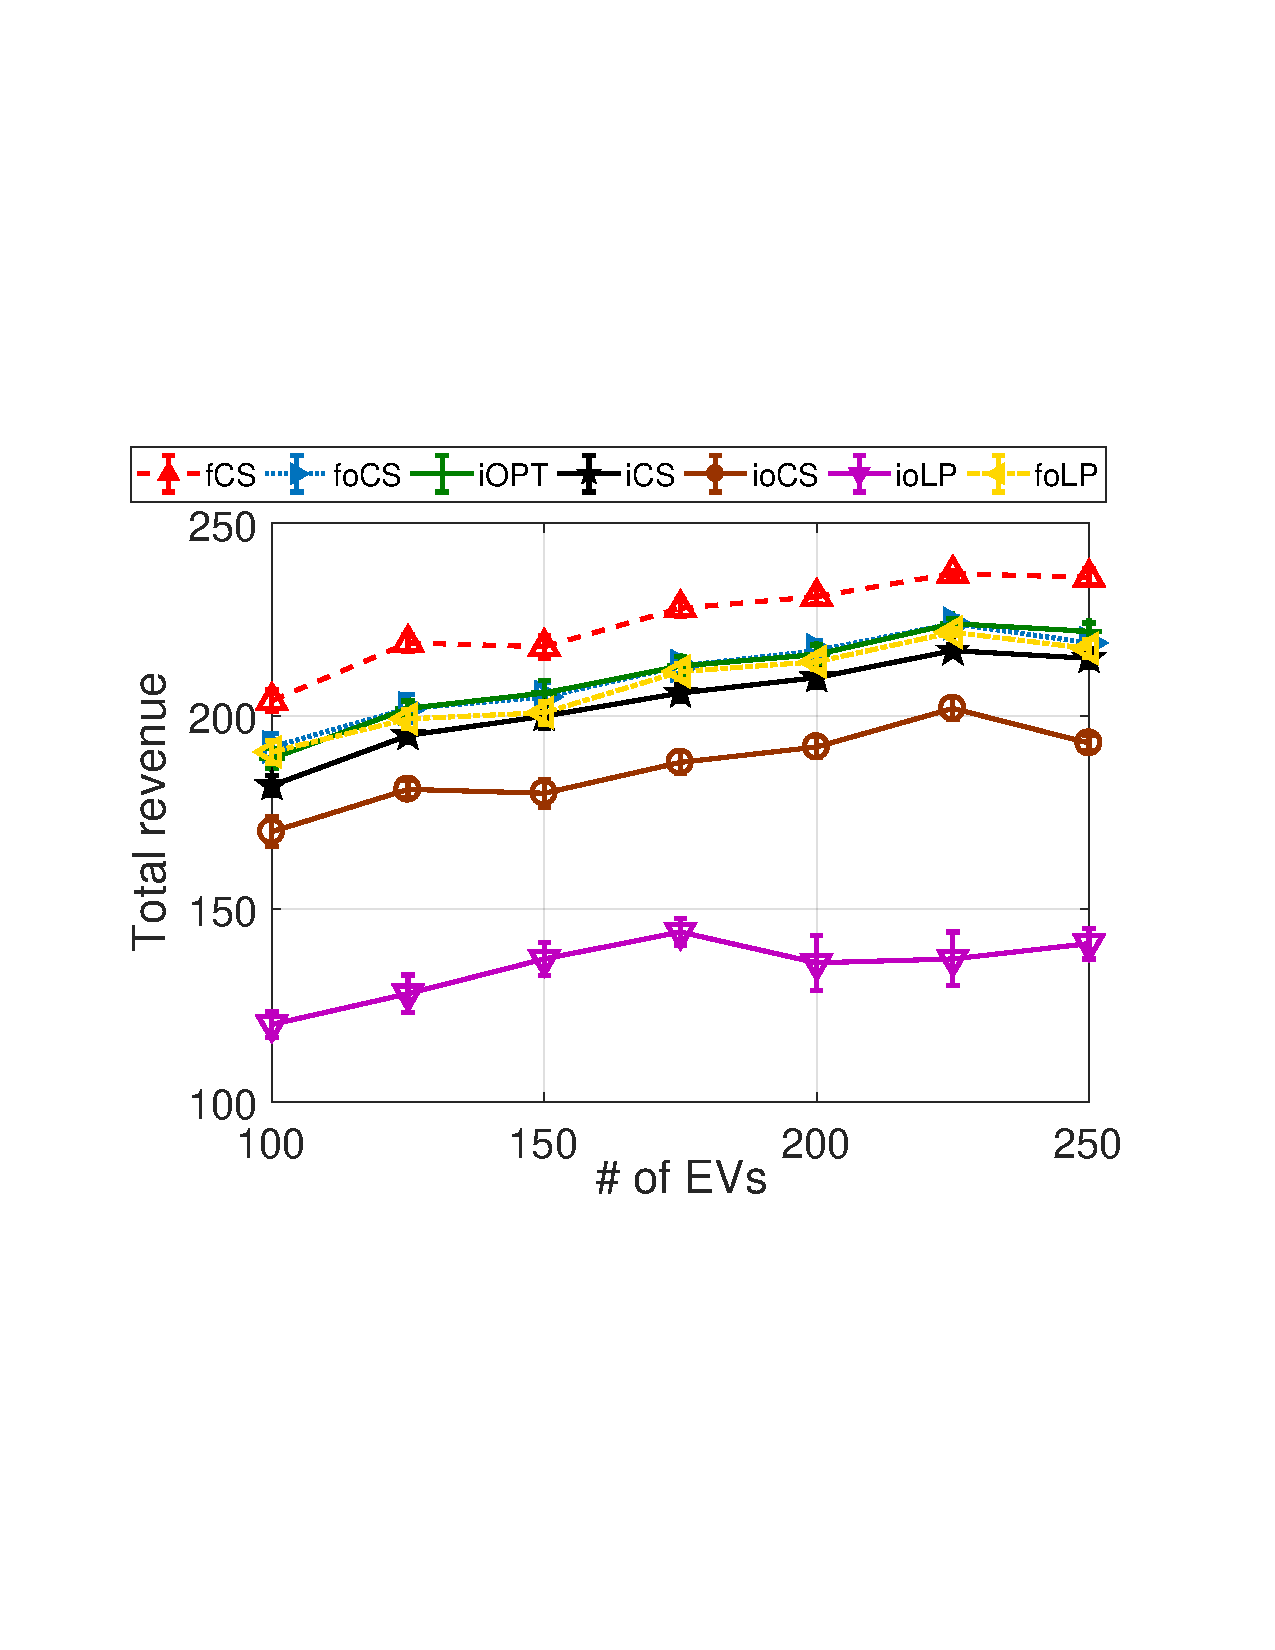
\includegraphics[width=\textwidth]{V-N-M2.pdf}
						\caption{\revv{$m=2$}}
						\label{fig:V-N-M2}
					\end{center}
				\end{subfigure}
				\begin{subfigure}[b]{0.25\textwidth}
					\begin{center}
						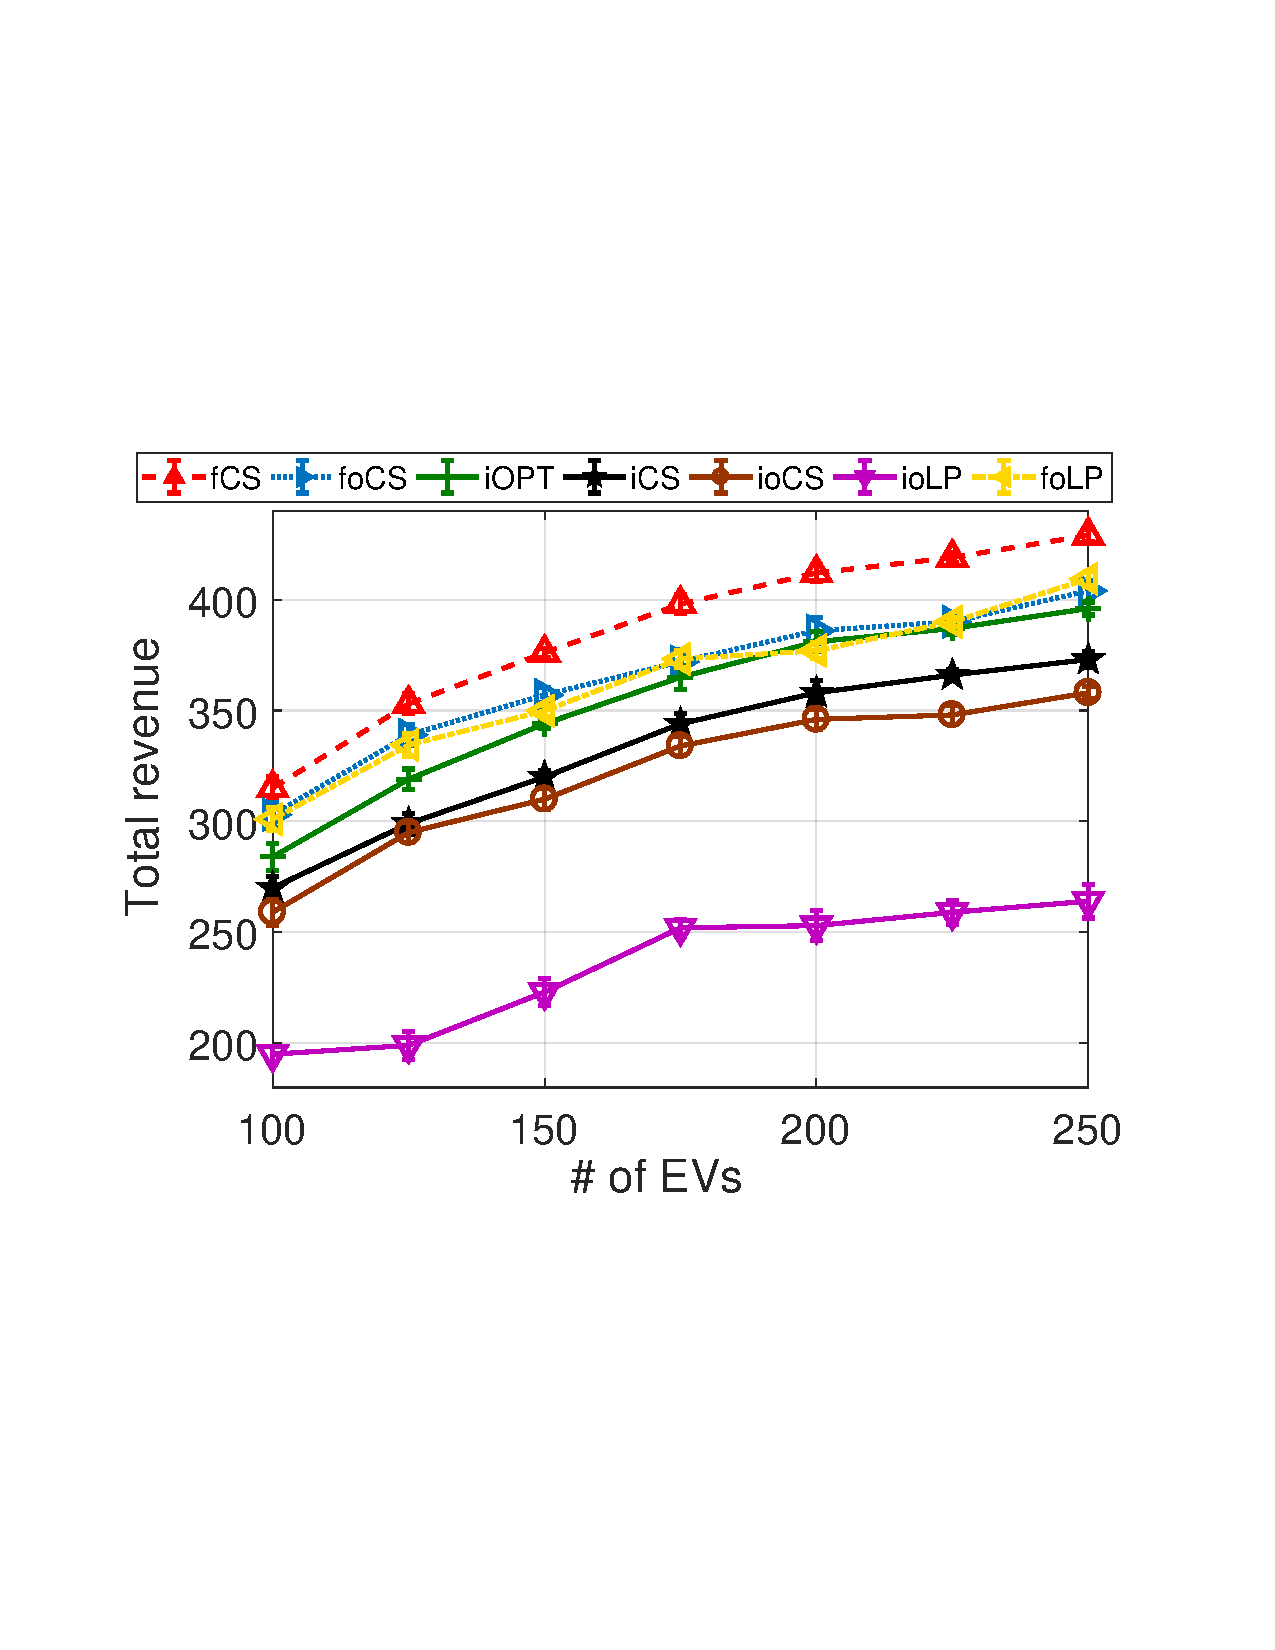
\includegraphics[width=\textwidth]{V-N-M4.pdf}
						\caption{\revv{$m=4$}}
						\label{fig:V-N-M4}
					\end{center}
				\end{subfigure}% 	
				\begin{subfigure}[b]{0.25\textwidth}
					\begin{center}
						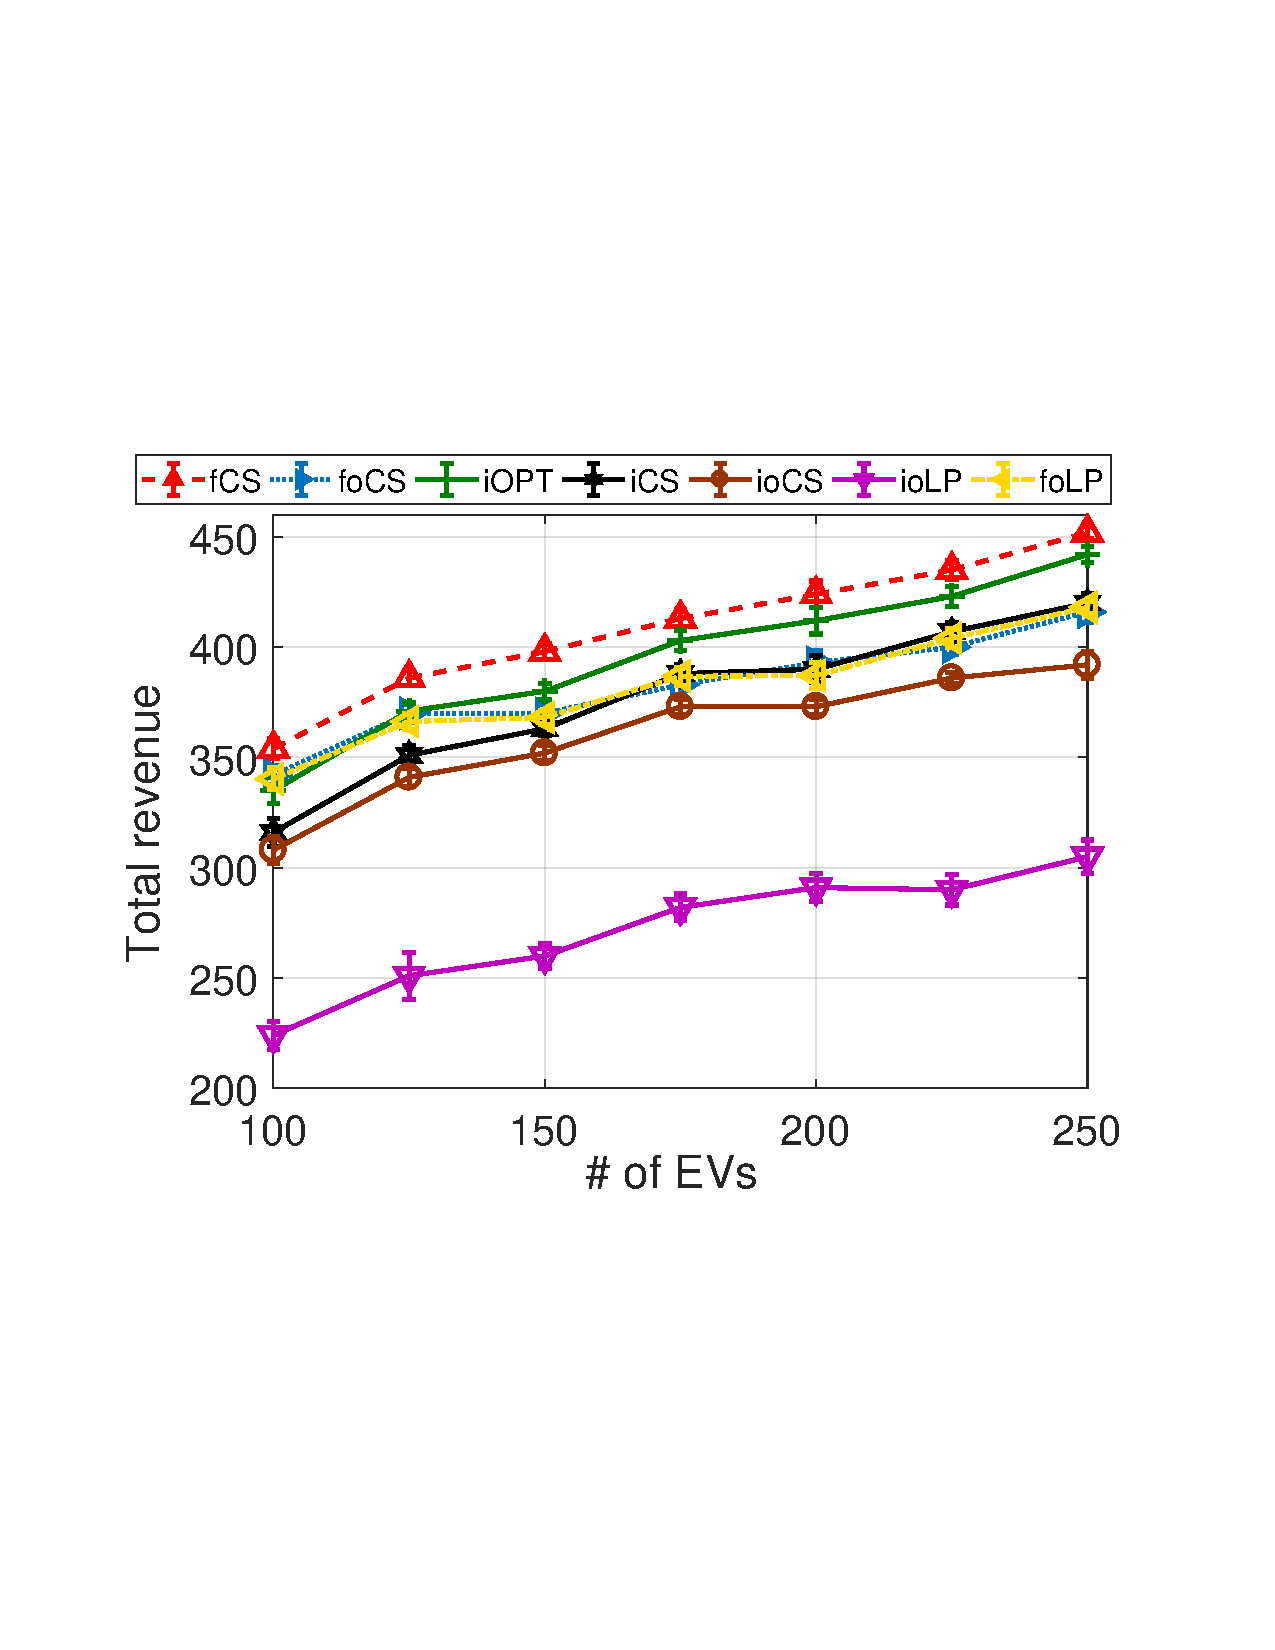
\includegraphics[width=\textwidth]{V-N-M8.pdf}
						\caption{\revv{$m=8$}}
						\label{fig:V-N-M8}
					\end{center}
				\end{subfigure}% 
				\caption{\revv{Comparison results for $2$, $4$, and $8$ CSs for fractional and integral revenue models.}} 
				\label{fig:V-N-M}
				\vspace{-3mm}
			\end{figure*}
%\subsection{Simulation Setup and Overview}
\textit{Simulation Setup and Overview:} We consider charging scheduling of EVs \revv{during a period of $12$ time slots of length $1$ hour (e.g., from $08$:$00$ to $20$:$00$)}. 
We gathered information of \revv{$12$} popular EV models in the market to use in the simulation. Each EV model is characterized by its battery capacity as shown in Table \ref{tb:models} and maximum charging rate. \revv{Tesla models can get charged with up to $100$ kW using Tesla super chargers. Also, all other models have rapid DC charging capability (up to $50$ kW) with CHAdeMO method. This setting for charging rates is in accordance with future DCFC systems that can have several fast DC chargers installed in the charging station.} 
%Battery capacity varies from \revv{$14$} kWh to \revv{$100$} kWh and the maximum charging rate from \revv{$3.3$} kW to \revv{$22$} kW. 
%As in \cite{Tang,Chen}, we assume that arrival times follow a Poisson distribution and parking times follow an exponential distribution.
% with the mean arrival and parking duration indicated in Table \ref{tb:a-d}. 
The peak intervals include $08$:$00$-$10$:$00$, $12$:$00$-$14$:$00$, and $18$:$00$-$20$:$00$ which is in accordance to NHTS survey~\cite{Santos, Tang}. \revv{The probability of arriving an EV in the peak hours is two times higher than the off-peak periods.
			Demands are uniform random values from 
			$[\frac{1}{2}U_i,U_i]$} where $U_i$ is the battery capacity for EV $i$ in Table~\ref{tb:models}. \revv{The deadline of each EV is set according to slackness parameter $s$ (with default value of $1.2$), its demand and maximum charging rate of the battery as $d_i=a_i+\lceil \frac{D_is}{k_i} \rceil -1$.} 
%			The minimum electricity cost is $\$0.11$ per kWh based on US national electricity price average~\cite{kWhcost}. In our setting, users can submit higher prices than the minimum price in order to ensure receive their requested demand. 
			\revv{EVs are assigned to different CSs randomly and given as input to the algorithms. The willingness to pay by each user for one kWh of power is a random uniform number from interval $[\frac{1}{2} z,\frac{3}{2}z]$ where $z=\$0.11$ is national average price of electricity in the US\cite{kWhcost}.}			
			%The default value of local peak constraint is \rev{$100$} kW and the global peak constraint is \rev{$200$} kW. We investigate the effect of this parameter in~\cite{alinia2017online}. 
			In the simulation, the results are plotted with $95\%$ confidence level and each point represents average result of $50$ random scenarios. Table \ref{tb:comparisons} explains the comparison algorithms \revv{including current implemented algorithm in Caltech ACN referred to as \iolp \cite{lee2016adaptive} and its adapted version for the fractional revenue model \folp. The \iolp and \folp algorithms runs as follows: at each time slot assume that there will be no further arrivals and solve the optimization problem (e.g., by commercial solvers) for the current set of EVs and their remaining demands. In Table \ref{tb:comparisons}, the letters ``\textsc{i}'', ``\textsc{f}'' and ``\textsc{o}'' in front of the algorithms' name refer to integral, fractional and online types, respectively.} 
			
			The measured performance metrics are total revenue, percentage of EVs that received all their demand, and total peak. \revv{To calculate optimal solution in integral revenue model, we used Gurobi solver \cite{optimization2013gurobi}.} 
			
						
\begin{table}[!t]
				\centering
				\caption{\revv{EV models and their battery capacity.}}
				\label{tb:models}\revv{
				\begin{tabular}{ | l| c | l| c |}
					\hline
					\textbf{Model} & \textbf{Battery} & \textbf{Model} & \textbf{Battery} \\ \hline\hline    
				Mitsubishi i-MiEV & $16$ kWh & Citroen C-Zero & $14$ kWh \\ \hline
				Peugeot iOn  & $16$ kWh & Honda Clarity & $25.5$ kWh\\\hline
				Hyundai Kona & $64$ kWh & Nissan LEAF & $40$ kWh \\ \hline
				Hyundai Ioniq & $28$ kWh & BMW i3 & $22/33$ kWh \\ \hline
				Tesla Model S/X  & $60/100$ kWh & Kia Soul EV  & $27$ kWh\\\hline
				\end{tabular}}
			\end{table}
			
%\begin{table}[h]
%				\centering
%				\caption{Arrival rates and mean parking times.}
%				\label{tb:a-d}
%				\begin{tabular}{ | l | c | c |}
%					\hline
%					\textbf{Interval} & \textbf{Arrival rate} & \textbf{Mean parking time} \\ \hline\hline    
%					$08$:$00$-$10$:$00$&  $14$&$10$\\\hline  
%					$10$:$00$-$12$:$00$&  $10$&$1/2$\\\hline 
%					$12$:$00$-$14$:$00$&  $20$&$2$\\\hline 
%					$14$:$00$-$18$:$00$&  $10$&$1/2$\\\hline
%					$18$:$00$-$20$:$00$&  $20$&$2$\\\hline
%					$20$:$00$-$24$:$00$&  $10$&$10$\\\hline
%					$24$:$00$-$08$:$00$&  $0$&$0$\\\hline
%				\end{tabular}
%\end{table}

\begin{table}[!t]
\centering
\caption{Acronyms for the algorithms}
\label{tb:comparisons}
\begin{tabular}{ | l| p{6cm}|}
\hline
\textbf{Notation} & \textbf{Description} \\ \hline\hline
\textsc{iOpt} & Optimal value under integral revenue model\\ \hline 	 
\ics & Proposed offline algorithm for \MCSP under integral revenue model\\ \hline
\fcs & Proposed \emph{optimal} algorithm for \MCSP under fractional revenue model\\\hline 
\iocs & Proposed online algorithm for \MCSP under integral revenue model\\ \hline
\focs & Proposed online algorithm for \MCSP under fractional revenue model\\ \hline
\iolp & Algorithm in \cite{lee2016adaptive} (works under integral revenue model)\\ \hline
\folp & Adaptation of algorithm in \cite{lee2016adaptive} for fractional revenue model\\ \hline
GreedyRTL & The algorithm in \cite{Jain} for single station scenario without global peak 			constraint (works under integral revenue model)\\\hline				
\end{tabular}
\end{table}
			%to simulate: Fig. 1 with M=1,4,8			
			\begin{figure*}[t!]	
				\centering
				\begin{subfigure}[b]{0.25\textwidth}
					\begin{center}
						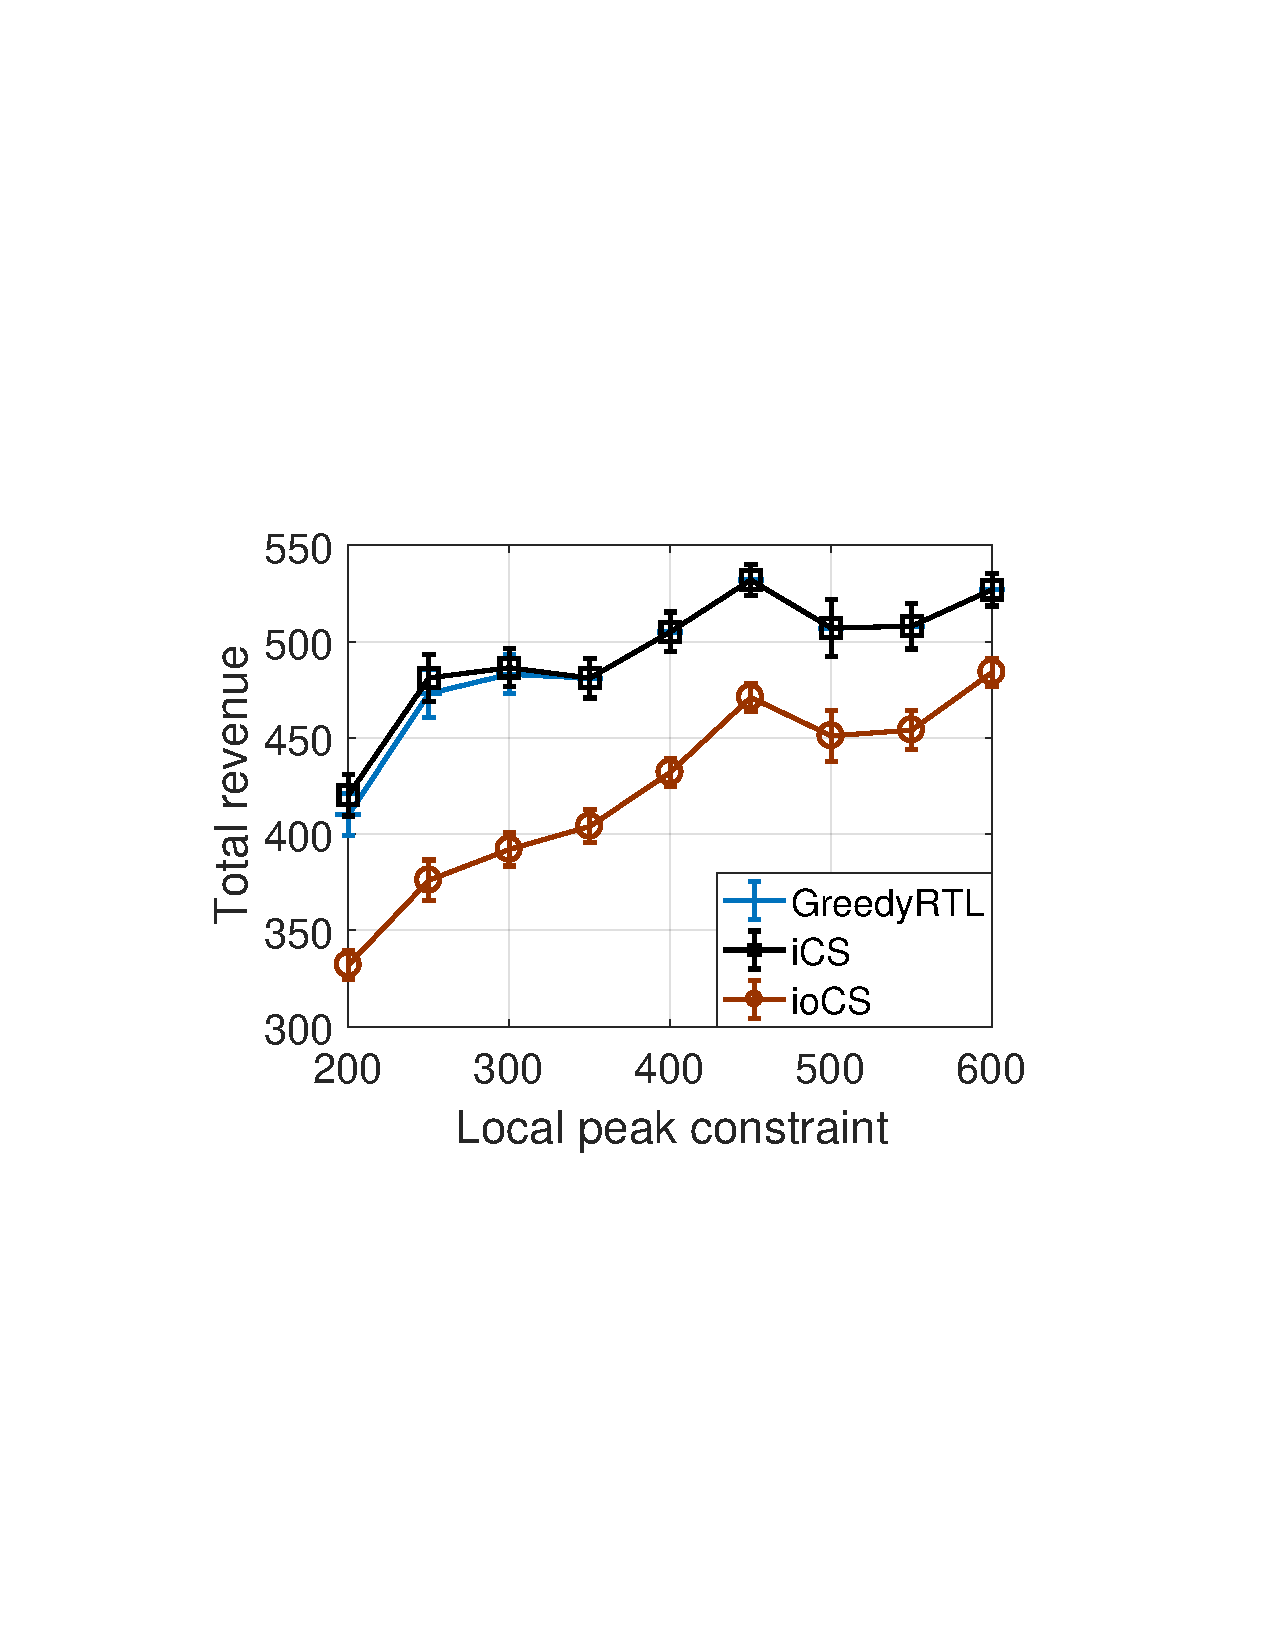
\includegraphics[width=\textwidth]{v-c.pdf}
						\caption{\revv{Total revenue}}
						\label{fig:v-c}
					\end{center}
				\end{subfigure}%
				%\hspace{4mm}
				\begin{subfigure}[b]{0.25\textwidth}
					\begin{center}
						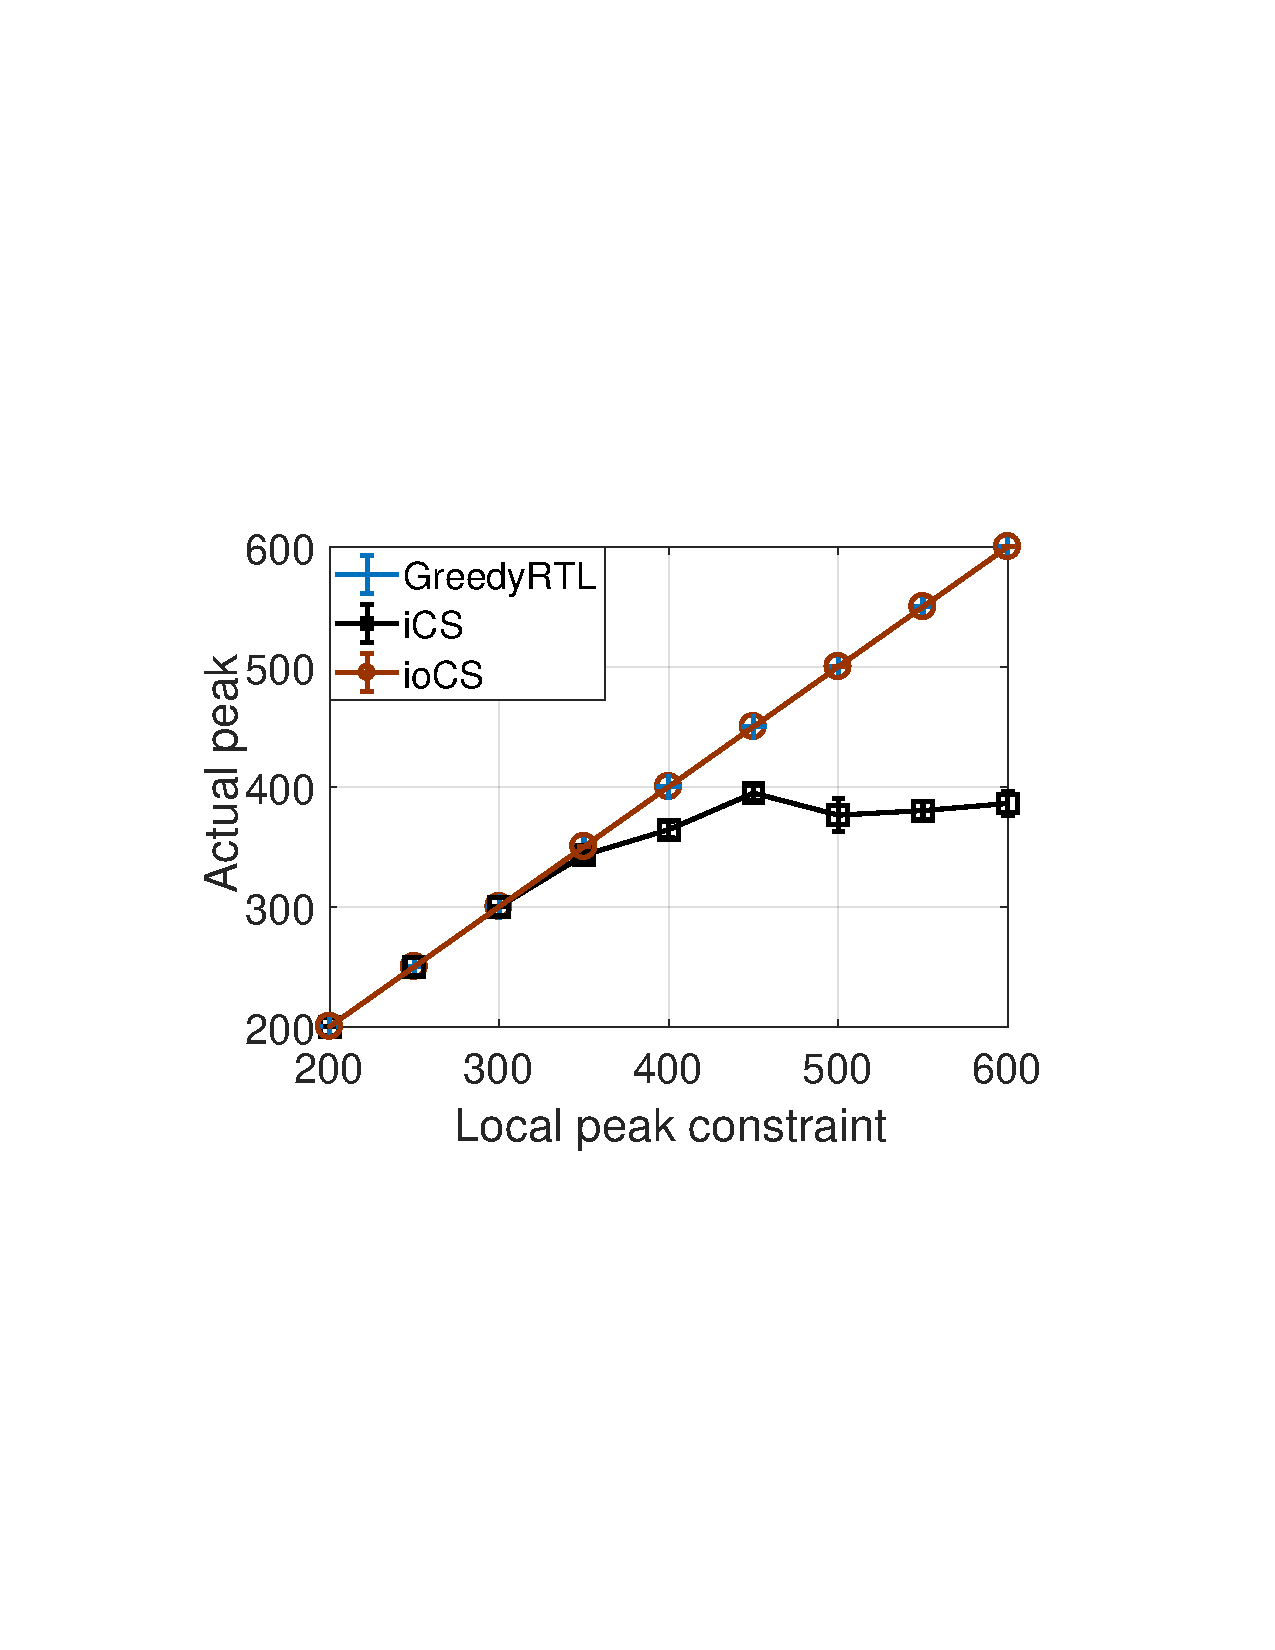
\includegraphics[width=\textwidth]{p-c.pdf}
						\caption{\revv{Actual global peak} 
%							($p^{\mathsf{total}}=480$)
}
						\label{fig:p-c}
					\end{center}
				\end{subfigure}%  
				%\hspace{4mm}
				\begin{subfigure}[b]{0.25\textwidth}
					\begin{center}
						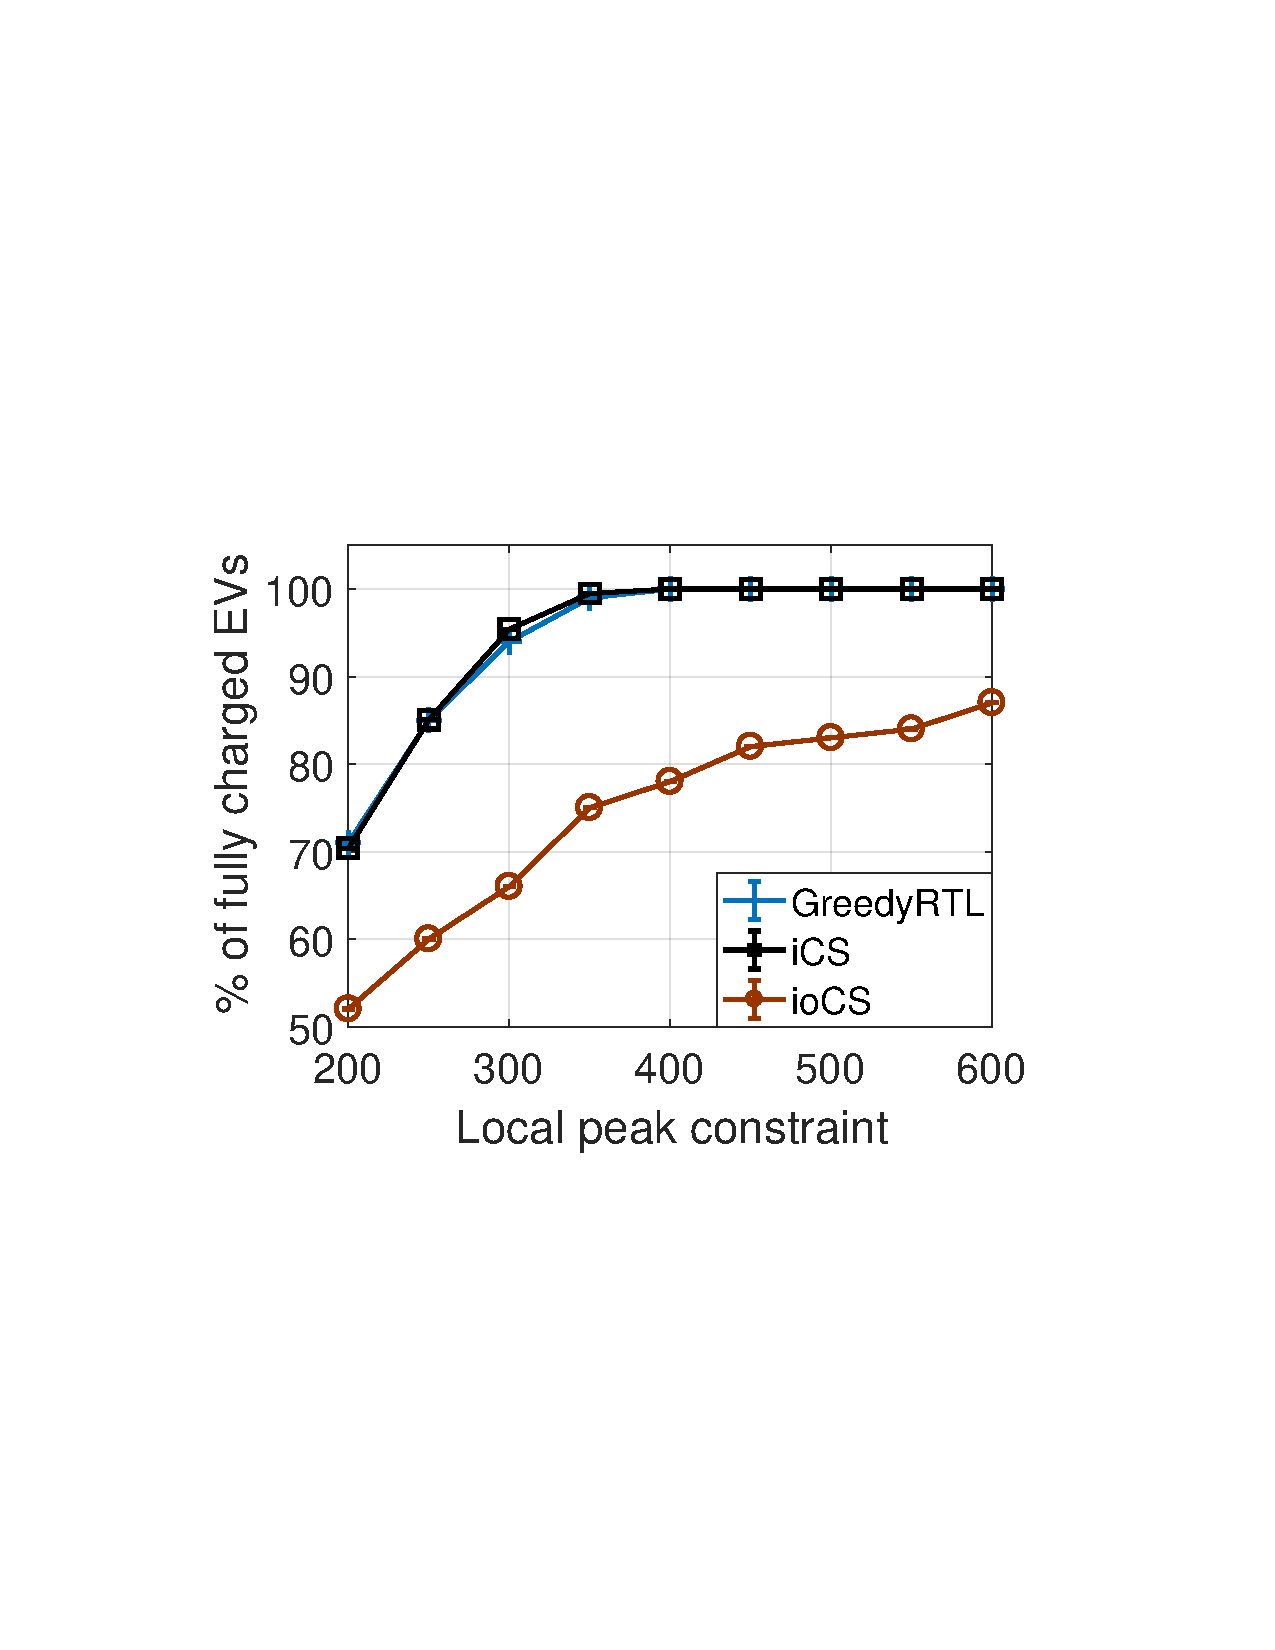
\includegraphics[width=\textwidth]{acc-c.pdf}
						\caption{\revv{\% of full charged EVs}}
						\label{fig:acc-c}
					\end{center}
				\end{subfigure}% 				
				\caption{\revv{Comparison in terms of total revenue, actual peak, and percentage of fully charged EVs by varying local peak value}.} 
				\label{fig:peak_local}
			\vspace{-4mm}
			\end{figure*}
\textit{\revv{Evaluation Based on Total Revenue}:}
\revv{Fig. \ref{fig:V-N-M} depicts the comparison results based on total revenue under fractional and integral models} while the total number of EVs increases from \revv{$100$ to $250$} for $2$, $4$, and $8$ CSs. \revv{The local and global peak constraints are set to $50$ kWh and $200$ kWh, respectively.}

The proposed algorithms compared to the optimal offline solution of integral model ($\textsc{iOPT}$) and $\iolp$.%%% which is the running online algorithm in the Caltech ACN \cite{lee2016adaptive}. 
%The proposed algorithms for fractional revenue model, \fcs and \focs, are compared to fractional version of OLP algorithm (referred to as \folp), which is implemented in Caltech ACN  (see~\cite{alinia2017online} for details). 
Recall that \fcs is optimal offline solution. The notable observations  are  as  follows:  (i)  the  general  trend in scenario of Fig.~\ref{fig:V-N-M} is that  by increasing  the  number  of  EVs,  total  revenue  increases.  This is because with more number of EVs, the scheduler has more freedom to choose more valuable EVs. (ii)  as  explained in Section~\ref{sec:fractional}, under fractional charging model, better results are expected due to increased scheduling flexibility in CSs. According to the simulation data that we extracted from Fig.~\ref{fig:V-N-M}, the gain obtained by \fcs and \focs in Fig. \ref{fig:V-N-M} are respectively \revv{$12\%$ and $10\%$} more than the gain of the \ics and \iocs. (iii) \revv{In Fig. \ref{fig:V-N-M2} and Fig. \ref{fig:V-N-M4}, sum of the local peaks is less than or equal to the global peak while in Fig. \ref{fig:V-N-M8} this sum is two times greater than the global peak. Consequently, the total revenue significantly improved when the number of CSs is increased from $2$ to $4$ while there is a slight improvement from $4$ to $8$ CSs as the global peak constraint prevents the algorithms from charging more EVs.}
 (iv) in integral revenue model, the proposed \iocs algorithm acts significantly better than \iolp. In particular, \iocs improves \iolp by \revv{$38\%, 36\%$, and $32\%$} for $m=2$, $m=4$ and $m=8$, respectively. \revv{In fractional revenue model, however, there is a very slight difference between \focs and \folp.}
 %We highlight that \iocs (\focs) is also better choice in terms of the algorithm complexity compared to \iolp (\folp).
(v) \ics approximates \textsc{iOpt} by \revv{$97\%$, $94\%$, and $95\%$} for $m=2$, $m=4$, and $m=8$, respectively. On average, \iocs is \revv{$90\%$} of \textsc{iOpt} and, \focs is \revv{$94\%$} of its optimal offline solution, \fcs.  
(vi) finally, the results depict that \ics achieves much better results in practice as compared to the theoretical approximation ratio that characterizes the performance in worst-case scenario.

%Also, there is a sharp decline in the gap between the online methods (i.e., \focs and \iocs) and the offline solutions (i.e., \textsc{iOpt}, \ics and \fcs).


			
\revv{\emph{Comparison Based on Actual Peak:}} The constraint set in the \MCSP assures that any feasible solution respects the local and global peak constraints.
% i.e., at each time slot, the electricity consumed by station $j$ is less than or equal to $p_j$ and accumulative charging rate of all stations are less than or equal to $p^\mathsf{total}$ (note that there is no assumption that $\sum_j p_j\leq p^\mathsf{total}$, in general). 
An efficient scheduling algorithm may take a further step by not only satisfying the peak constraints but to further reduce the peak as much as possible. The proposed offline algorithms (i.e., \ics and \fcs) apply valley-filling policy to reduce the peak. The  online algorithms (i.e., \iocs and \focs) do not apply the same policy as they do not have future knowledge to be able to balance allocated resources. 
%Besides, due to uncertainties in future EV charging load in online scheduling design, it is a natural heuristic to charge EVs at earliest time.
% (i.e., setting the charging rates to the maximum feasible value at each time slot) as applied by \iocs an \focs. 
%This heuristic works well as the uncertainty in EVs' arrival time and demands may not give a second opportunity to the scheduler to charge the current EVs at the next slots. Therefore, although it is expected that \iocs and \focs have higher peak values compared to the offline algorithms, the idea of valley-filling can decrease their average response time.
% (see~\cite{alinia2017online} for the extended version of experiments).
To investigate the effect of employed valley-filling strategy, we conducted a set of simulations by varying local peak constraints. 
%from $50$ kWh to $120$ kWh and $200$ EVs. 
The results of \ics is compared to \iocs and GreedyRTL~\cite{Jain} where the latter is an approximation scheduling for single station scenario with EVs having same arrival time (see the explanations after formulating the \MCSP in Section \ref{sec:problem}). 
%The GreedyRTL algorithm works under integral revenue model. Therefore, results for \fcs and \focs are not plotted. 
%Since GreedyRTL assumes all EVs arrive at the same time, we set all arrival times to $1$. Moreover, we assume that global peak constraint is big enough (i.e., $\sum_{j=1}^m p_j\leq p^\textsf{total}$) such that the solution of GreedyRTL is feasible. We run GreedyRTL in each CS separately and combine the results. 
The results are shown in Fig.~\ref{fig:peak_local}.  
Along with total revenue in Fig.~\ref{fig:v-c}, we also report total \emph{actual} peak in Fig.~\ref{fig:p-c} and percentage of fully charged EVs in Fig.~\ref{fig:acc-c}. 
%As a high level trend, the results show that as the peak values increase, total revenue, total actual peak, and the number of EVs who received all their demand increase.  
In Fig. \ref{fig:v-c}, the results for \ics and GreedyRTL are almost identical while \iocs is \revv{$90\%$} of the other two algorithms, on average. When \revv{$p_j\geq 400$}, the total revenue for \ics and GreedyRTL does not increase in Fig. \ref{fig:v-c} and percentage of fully charged EVs is $100$ for both algorithms according to Fig. \ref{fig:acc-c}. From this point and onward, the scheduling is not challenging for offline methods to obtain optimal answer because of resource sufficiency. However, it is still a challenge to control total actual peak for the system. As a result of valley-filling policy, the value of actual peak of \ics in Fig. \ref{fig:p-c} remains almost unchanged for \revv{$p_{j}\geq 400$}.  \iocs and GreedyRTL, however, continuously increase the peak demand, since they are not using any peak shaving approach.
% and only try to maximize total revenue. 
%According to Fig. \ref{fig:p-c}, \iocs always reaches to the maximum peak of $\sum_j p_j$.
			
			
%A glance at Table \ref{tb:models} shows that in general, an EV needs a minimum time of $2$ hours to get $70\%$ of its battery capacity if charging rate is set to the maximum value. However, CSs are allowed to preempt the charging at any time and set charging rate any value lower than the maximum rate. Therefore, average response times can be higher as it can be seen in Fig. \ref{fig:rt-c}.
			
%\begin{figure}[t]	
%\centering
%				\begin{subfigure}[b]{0.25\textwidth}
%					\begin{center}
%						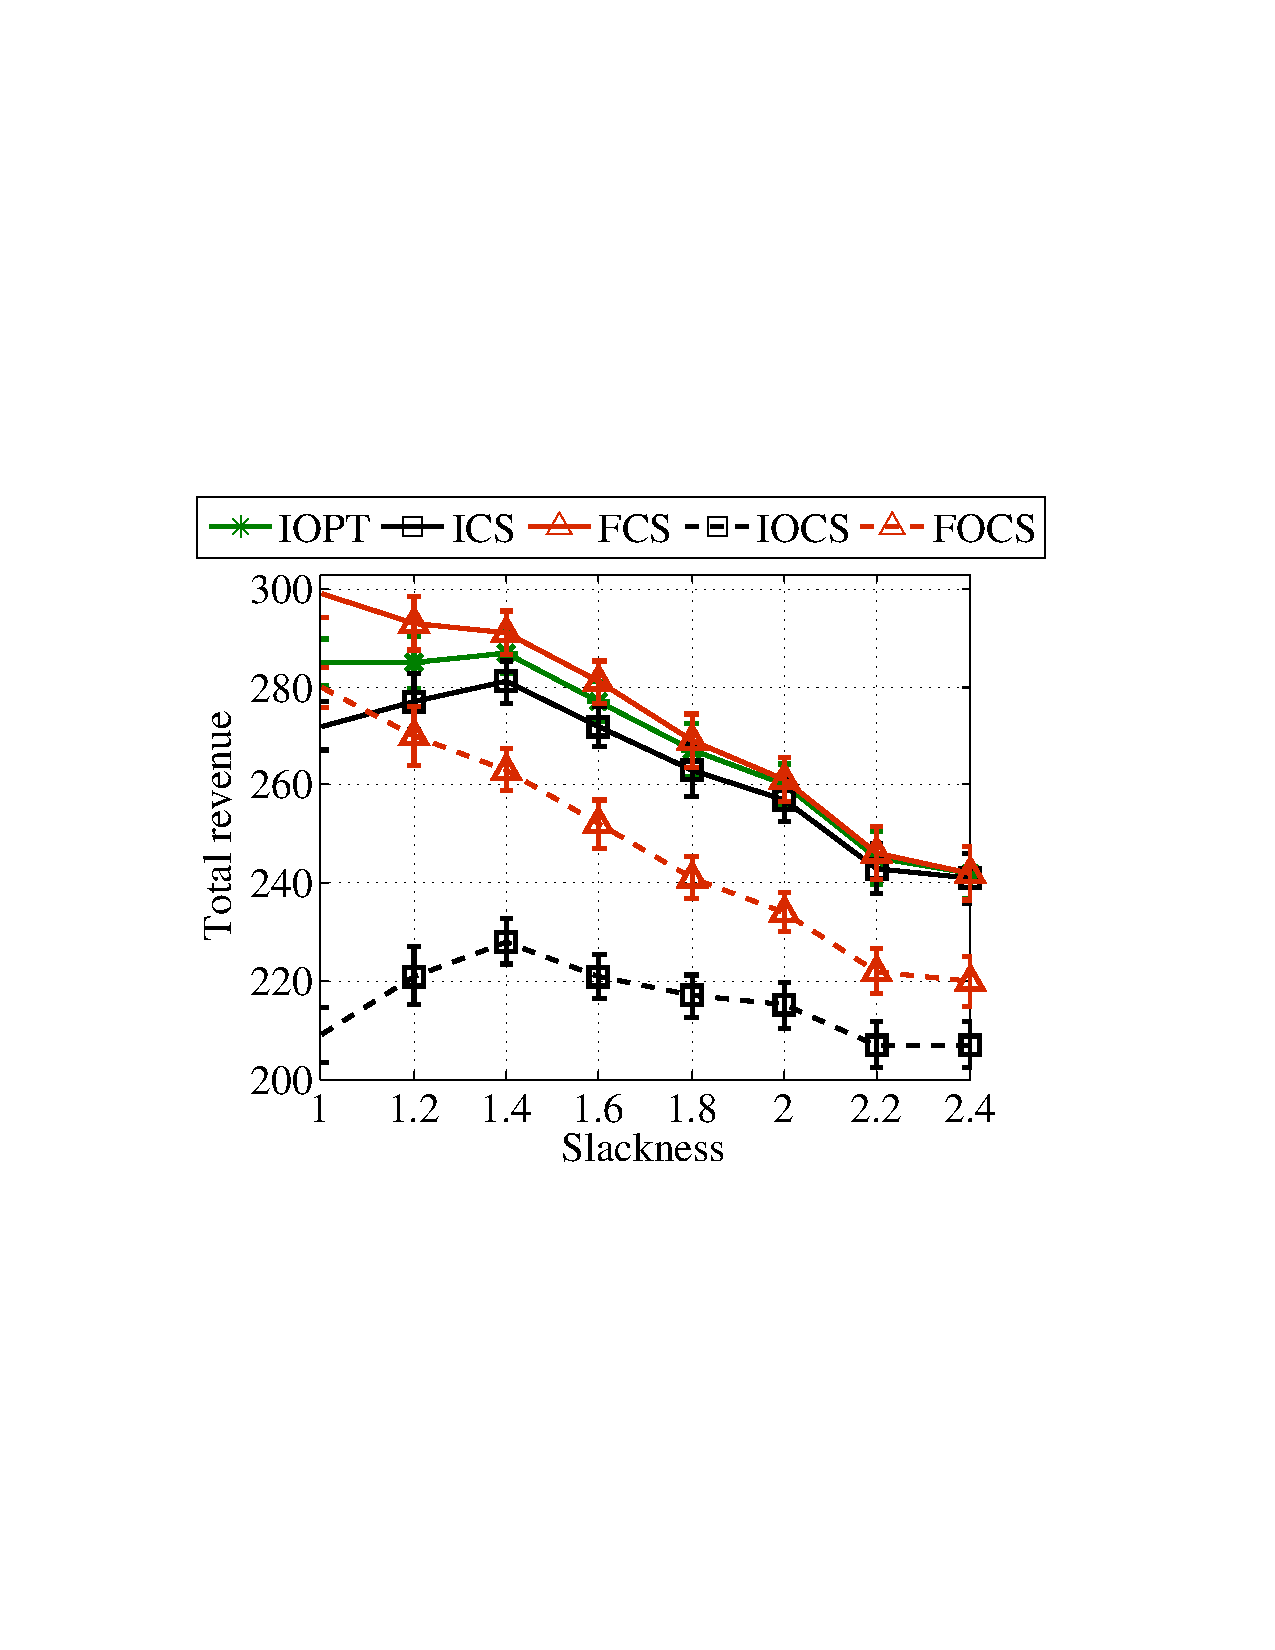
\includegraphics[width=\textwidth]{v-s-method1.pdf}
%						\caption{Total revenue (\$)}
%						\label{fig:v-s-method1}
%					\end{center}
%				\end{subfigure}%				
%				\begin{subfigure}[b]{0.25\textwidth}
%					\begin{center}
%						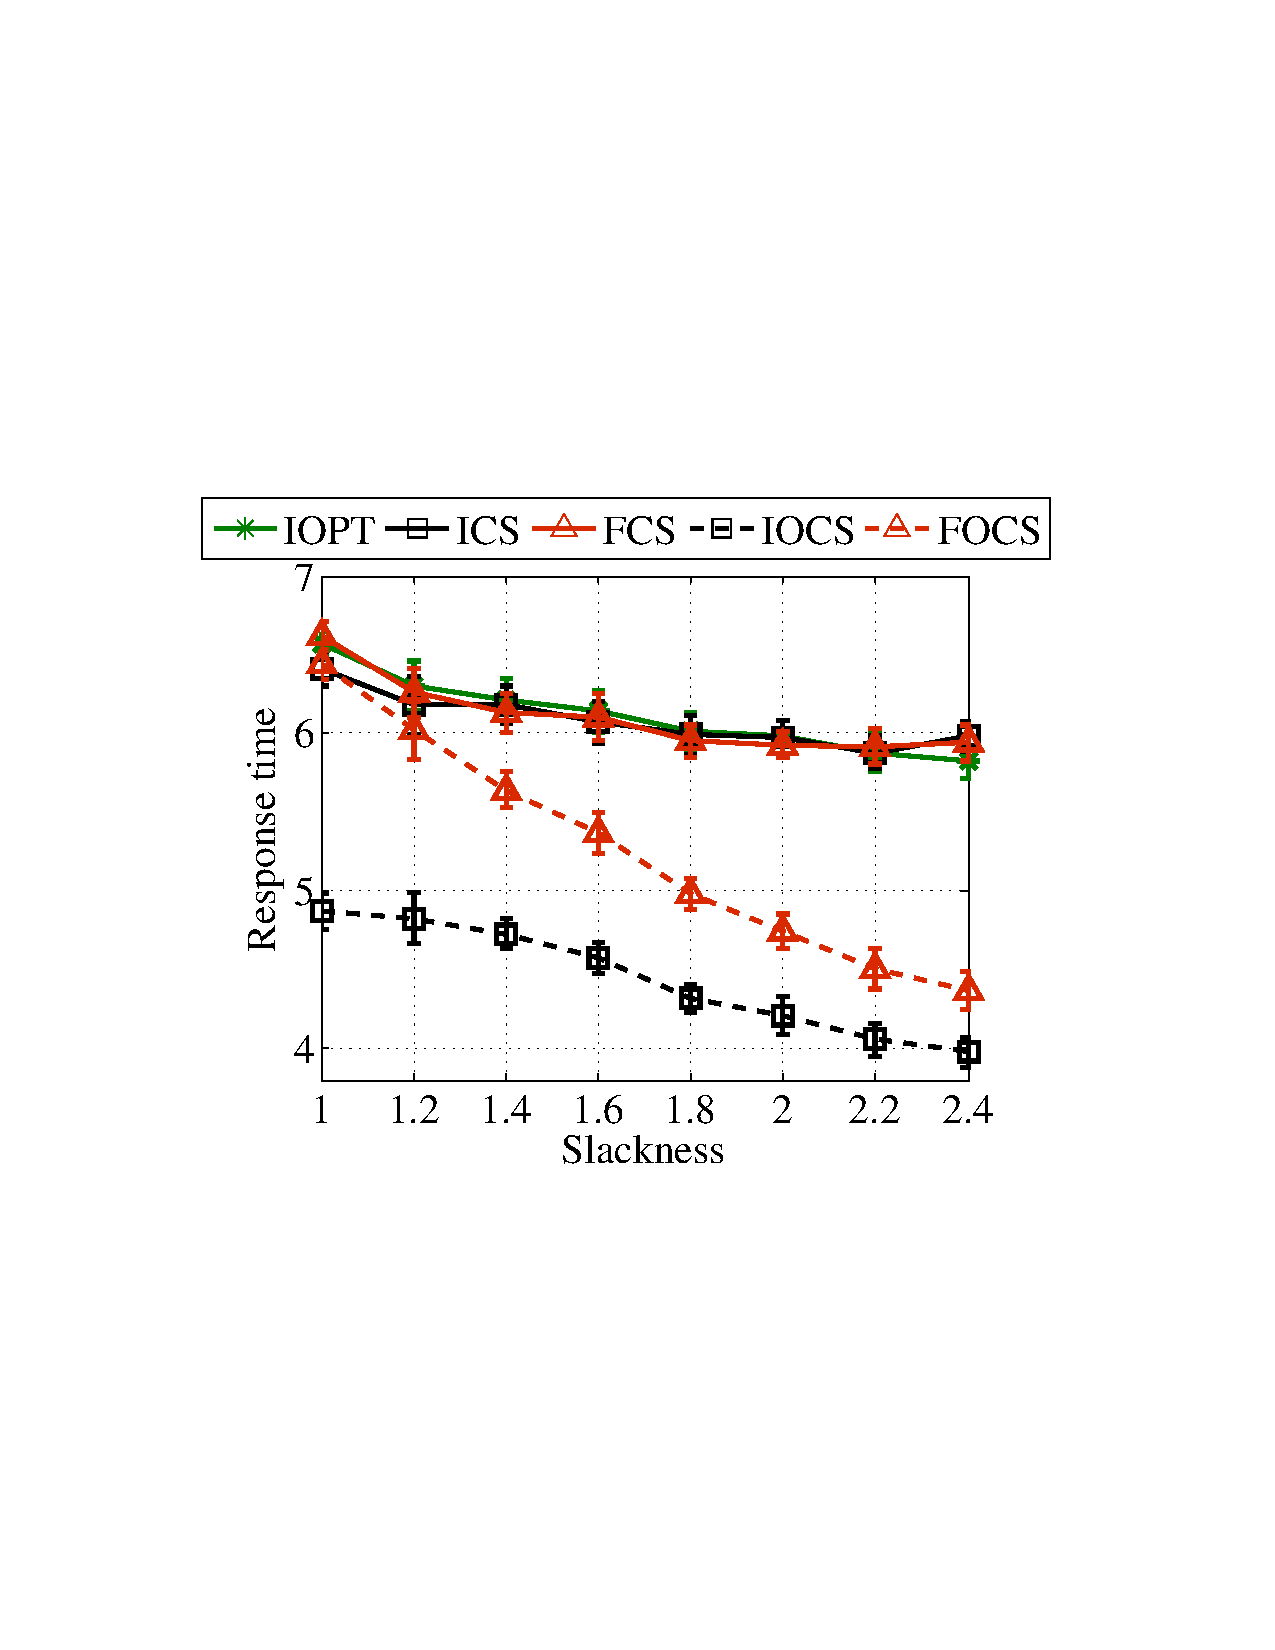
\includegraphics[width=\textwidth]{rt-s-method1.pdf}
%						\caption{Response time (hr))}
%						\label{fig:rt-s-method1}
%					\end{center}
%				\end{subfigure}%  
%\caption{The impact of slackness parameter on total revenue and response time when users react by adjusting their demand.} 
%\label{fig:slackness1}
%\end{figure}
			
%\subsection{The Impact of Slackness Parameter}
%\label{sec:sim:slack}
%This section discusses on the benefits and disadvantages that can be brought by using slackness parameter. To give the charging scheduler more flexibility, a slackness parameter $s\geq 1$ is used and set by the system designer. 
%Recall that charging profile of EV $i$ is feasible if $D_i\leq k_i\frac{d_i-a_i+1}{s}$ holds. Since users have no control on the slackness parameter and the maximum charging rate, they must adjust their demand and availability according to the imposed slackness value. Based on the charging profile feasibility equation, when the slackness value increases users have two choices to react: (i) decrease the demand and depart at the desired deadline or, (ii) extend the deadline and receive the desired demand. In the remaining of this section, we investigate the effects of either case by simulation. To have a clear picture of effects caused by slackness parameter, we generated $100$ initial charging profiles $\langle a_i,d_i,v_i,D_i,k_i\rangle$ for $100$ EVs randomly and uniformly chosen from $10$ different models in Table \ref{tb:models} such that the initial profiles are set up assuming that the CS allows the charging operations to be finished at earliest possible time (i.e., $\frac{D_i}{k_i}$) with $s=1$. For each EV, its demand is randomly chosen from $25\%$ to $100\%$ of its battery capacity and departure in  interval $[a_i+\frac{sD_i}{k_i},T]$, where $a_i+\frac{sD_i}{k_i}$ is the earliest feasible deadline. Then, the EVs are uniformly assigned to $4$ CSs and should choose one of the above strategies to submit a feasible demand according to imposed slackness. 
%\begin{figure}[t]	
%\centering
%							\begin{subfigure}[b]{0.234\textwidth}
%								\begin{center}
%									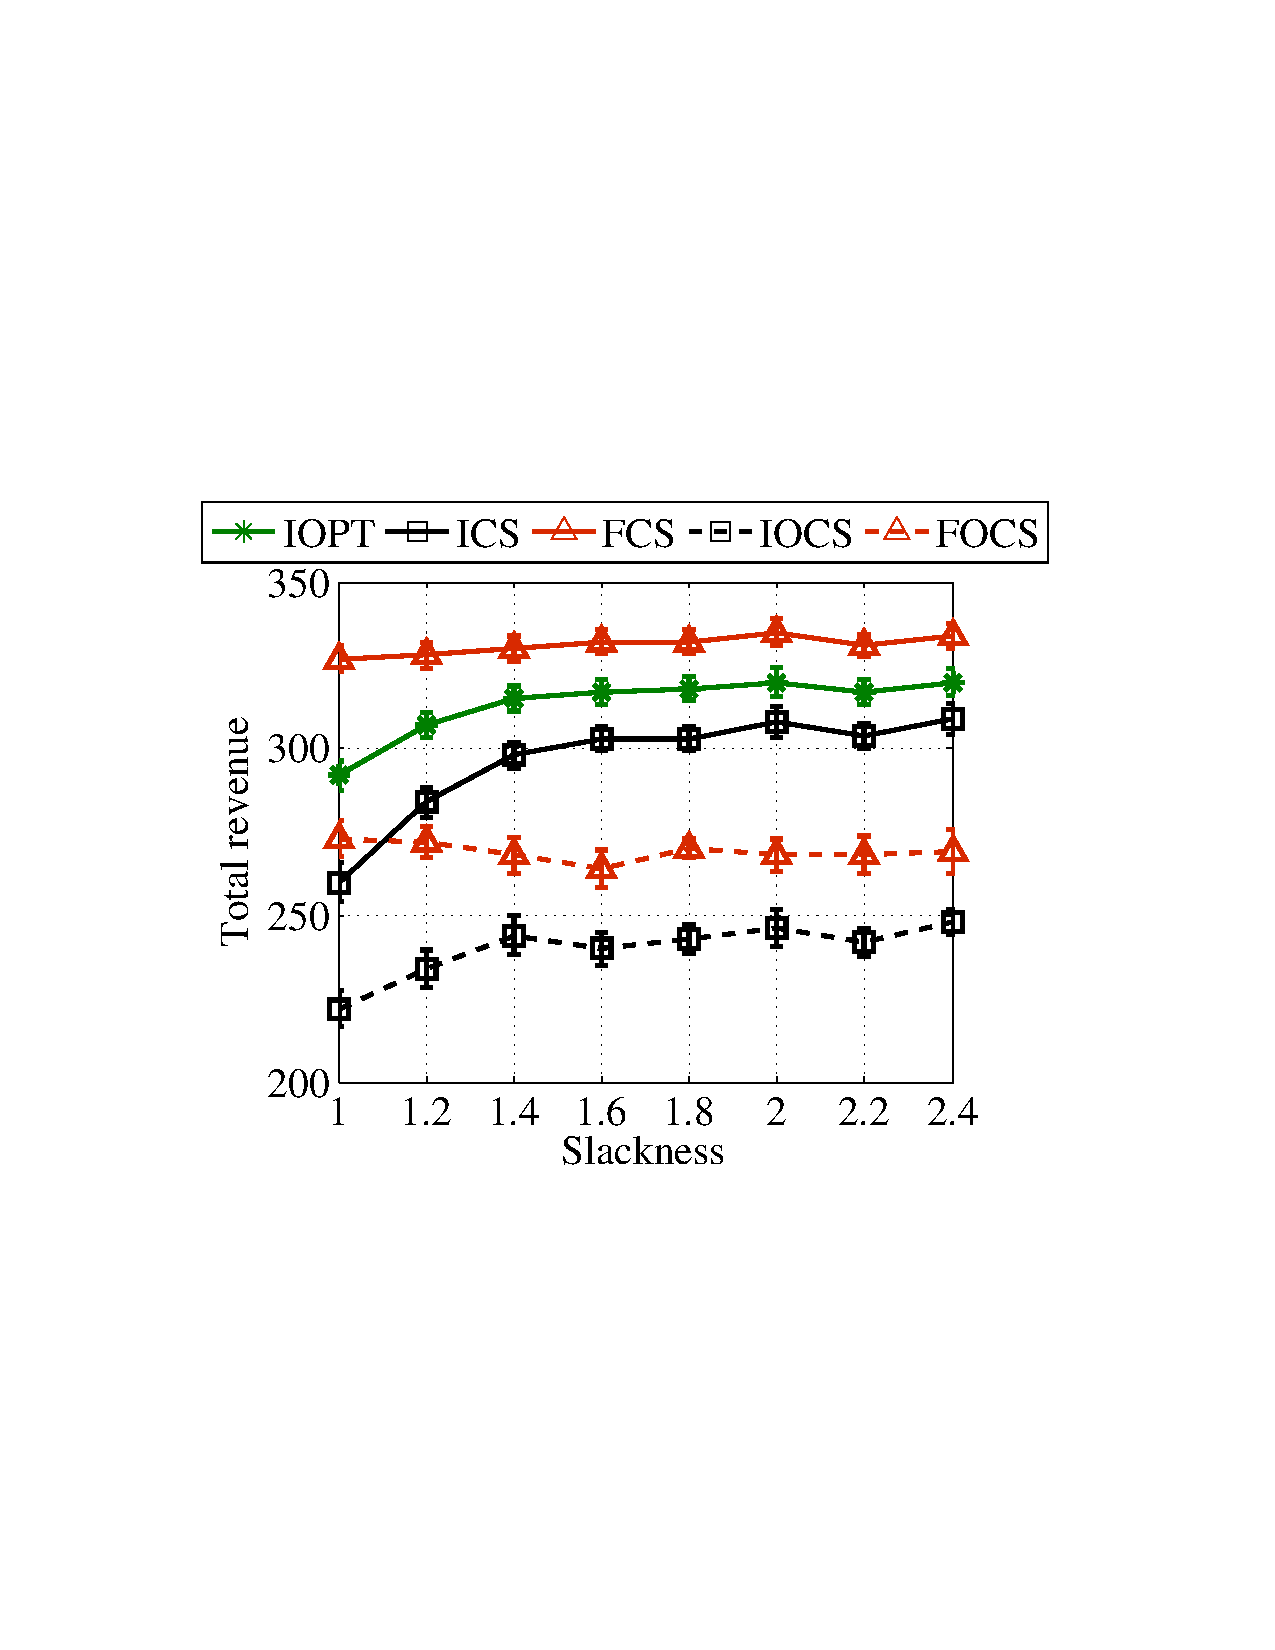
\includegraphics[width=\textwidth]{v-s-method2.pdf}
%									\caption{Total revenue (\$)}
%									\label{fig:v-s-method2}
%								\end{center}
%							\end{subfigure}%
%							\hspace{1mm}
%							\begin{subfigure}[b]{0.236\textwidth}
%								\begin{center}
%									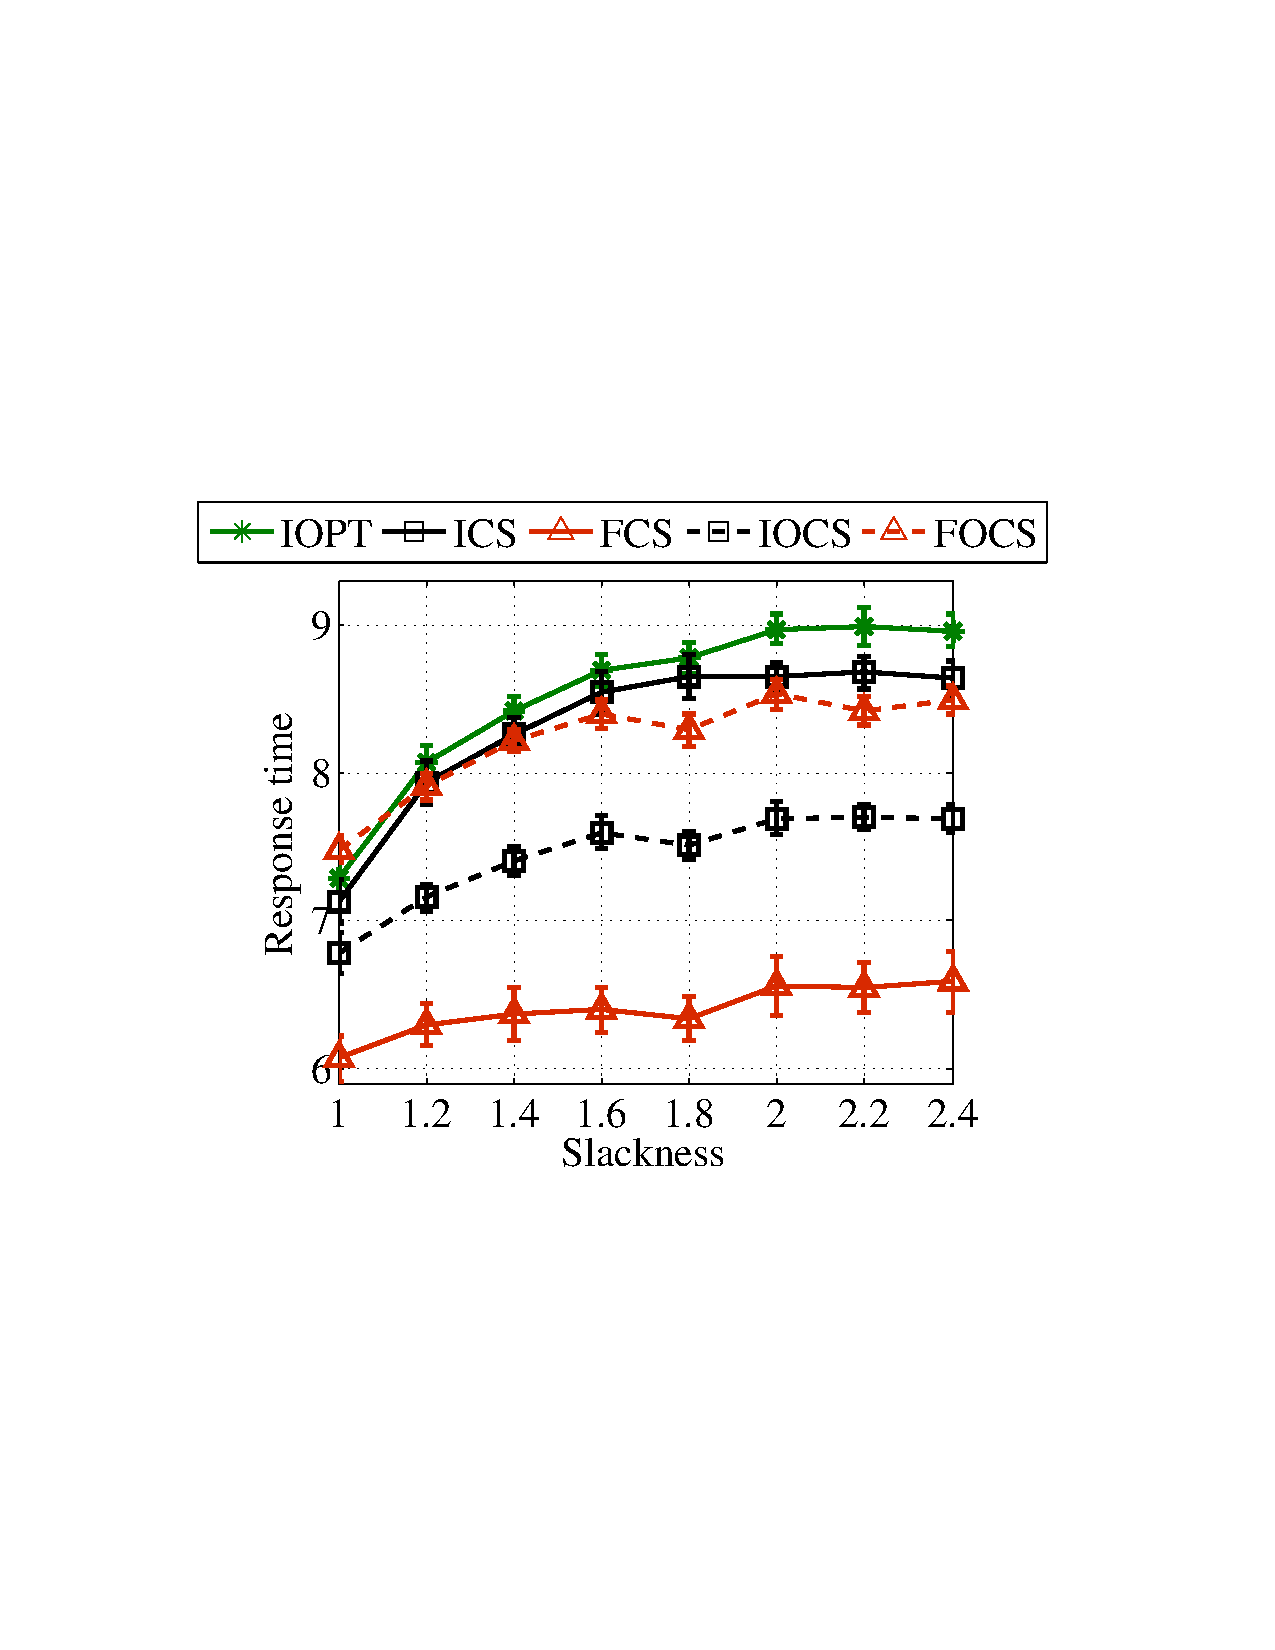
\includegraphics[width=\textwidth]{rt-s-method2.pdf}
%									\caption{Response time (hr)}
%									\label{fig:rt-s-method2}
%								\end{center}
%							\end{subfigure}% 
%							
%\caption{The impact of slackness parameter on total revenue and response time when users react by adjusting their deadline.} 
%\label{fig:slackness2}
%\end{figure}
%			
%\subsubsection{Case I- Adjusting Demands}
%In this case, if the initial charging profile of an EV does not reflect a feasible charging request based on the slackness parameter, the EV owner decreases its demand so it will be able to leave CS at its initial desired deadline. Note that the valuation of EVs decreases proportionally, as well. Fig.~\ref{fig:slackness1} depicts the result under this policy applied by users. As it can be seen in Fig. \ref{fig:v-s-method1} and Fig. \ref{fig:rt-s-method1}, the general trend is that both total revenue and average response time decrease when slackness value increases. This is justifiable based on users reaction. When users decrease their demand, less electricity is sold which results in less revenue. When total demand decreases, charging can be finished in shorter time which decreases response time. Therefore, if users choose the first policy (adjusting their demand), total revenue degrades while response time improves. Notice that for the algorithms working under integral revenue model (i.e., \textsc{iOPT}, \ics and \iocs) the total revenue increases with slackness parameter at first (when $s$ grows from $1$ to $1.4$) but then it decreases when the slackness increases more (for $s>1.4$). 
%In our view, this happens because increasing the slackness in integral revenue model makes it possible to \emph{fully} charge more EVs at the beginning as the demands decrease. However, when the slackness increases more, it results in opposite effect because the valuation of demands decreases along with the demands' size.	
%			\subsubsection{Case II- Adjusting Deadlines}
%			In this case, we assume that users are reluctant to decrease their desired demands. Instead, they can extend their departure. In Fig.~\ref{fig:slackness2} it can be observed that under this behavior of the users, the results are opposite as compared to the previous case (Fig.~\ref{fig:slackness1}). When deadlines are extended without demand decrement, the scheduler has more chance to compliance the demands through improved scheduling flexibility. Consequently, the total revenue increases by increasing slackness value while average response time degrades. 
%%Also observe the behavior of the online algorithms (i.e., \iocs and \focs) where both total revenue and response time decrease after a specific point that is $s=1.8$. When deadlines extend, more EVs have the opportunity of getting charged	
%					
%We can conclude that when total revenue is more important than the response time, the CS should impose small values of slackness for users that apply the policy of the first case and impose higher values of slackness for the users that apply the second policy. The conclusion is reverse for the case that the objective is to have lower response times. 

			%In fact, the slackness parameter controls the maximum demand or earliest deadline that an EV can submit to the system. Remember that demands are in interval $[\textrm{min}\{\frac{d_i-a_i}{sk_i},U_i\},U_i]$ for EV $i$ meaning that the maximum demand that an EV can submit decreases by increasing slackness parameter. A reduction in total demand result in lower charging costs. Therefore, the total revenue decreases with higher values of parameter $s$ as in Fig. \ref{fig:v-s}. 
			%Also, the percentage of EVs that received all of their requested demand increases based on the same fact. The main goal of this simulation is to observe that obtained theoretical result on approximation ratio is confirmed as optimality gap of the SCS algorithm reduces by increasing $s$ in Fig. \ref{fig:v-s}. 
\vspace{0.1mm}
\vspace{-4mm}
			\section{Conclusion}
			\label{sec:conclusion}
This paper proposed offline and online algorithms for the EV charging scheduling problem under fractional and integral revenue models in an adaptive charging network (ACN). The problem is different, and more challenging than the existing single station EV charging scheduling problems since it requires respecting the aggregate peak charging demand of the ACN. 
%More importantly, the problem is online in nature in the sense that the EVs arrive in time and the scheduler has no information regarding future arrivals. 
As the notable contributions, our proposed online algorithm for fractional revenue model achieves constant competitive ratio of $2$. Moreover, the offline integral algorithm achieves a theoretical bound on the optimality gap and approximates the optimum by $92\%$, on average in experiments. As a future work, we plan to study the problem under posted pricing mechanism where the charging station publishes the unit price of the power (which can be varied over time) and the users can accept or reject the offer.
\revv{Another interesting future direction is to tackle the EV charging scheduling in market-based scenarios where the prices change over time.}
%As a future work, we plan to analyze the truthfulness of the algorithms to make sure that it is a dominant strategy for the EV owners to declare their true valuations and availabilities.
\vspace{-4mm}

%\input{intro.tex}
%\input{rel.tex}
%\input{sys.tex}		
%\input{fraction.sol.tex}		
%\input{integral.sol.tex}
%\input{exp.tex}
%%%\vspace{0.1mm}
%\input{conc.tex}
%\newpage
%ss
%\newpage
%\pagestyle{empty}
\bibliography{ref}{}
\vspace{-2.8mm}
\bibliographystyle{ieeetr}

\appendix
%\vspace{-3mm}
\begin{comment}
\subsection{Related Work}
\label{sec:rel}
			
\subsubsection{Peak-Constrained EV Charging Scheduling}
\label{sec:rel:peakconstrained}			
There is an extensive literature on EV scheduling problem where most of them focused on single CS \cite{Tang,Wen} and the local and global peak constraints are usually omitted or only the local peak is considered.	As discussed in Section \ref{sec:problem}, the global optimal solution cannot be obtained by separately solving the single station problems. Hence, those solutions cannot be directly applied to our problem. 
			
A scenario that local and global peak constraints exist is the case that 
scheduling is required for a charging network for multiple CSs. Studies in \cite{He,Malhotra,Moradijoz,DWang,Zeng,Shaaban} addressed charging scheduling problem in multiple CSs. The authors in~\cite{He} tackled a global EV charging scheduling problem in a system consisting of a central controller and multiple local controllers to minimize total cost. However, there is no limit on the maximum peak demand that the system can tolerate. Consequently, the peak value can be arbitrary high depending on the total demand. 
This may increase the electricity bill of large costumers substantially mainly due to very high peak demand. In addition, high EV penetration level leads to high peak which may pose danger for the grid system \cite{DWang}. Besides, the charger devices installed in the CSs have limitation on the maximum power that they can transfer in each time unit~\cite{Tesla}. We solve the issue by constraining local and global peaks. However, to meet the peak constraints, it may not be feasible to respond to all charging demands. Consequently, only a subset of EVs can be charged~\cite{Xiang}, which is captured in our integral charging model. \cite{DWang} considered a multi-microgrid system with global peak constraint where each microgrid has a CS and the goal is to minimize the operating cost of the system and the exchanged electricity between microgrids and main grid. The authors assume that charging aggregators are able to forecast required information about individual EVs which may not represent a real scenario. A similar assumption is made in \cite{Zeng,Shaaban} where the objective is to maximize total utility of EVs and aggregators in a distribution network.
			
%\rev{To be removed: In our solution, we applied a priority based selection process (based on the EVs' valuation) to respond to the demands to make sure that total peak respects the constraints. The selection process can be made based on different criteria such as the value of each charging request \cite{Lee, Xiang} or the priority.}
			
			To avoid big billing cost in peak hours, \cite{Moradijoz} proposed a solution based on genetic algorithm to find optimal capacity and location of parking lots for serving demands in peak hours with the goal of maximizing total benefit of all stations. Although authors studied the problem under multiple CS setting, their solution is not applicable to our setting when the CSs are already set up. \cite{Malhotra} employed a similar model used in this paper, where both local and global peak constraints in a charging network are considered. The objective in \cite{Malhotra} is to maximize user convenience level which is different from the aim of the problem studied in this work. More importantly, the authors solve the single-slot problem, which fails to provide a general solution taking into account EVs' arrival and departure times which are considered in our study.
%			\subsection{Peak-minimizing EV Charging Scheduling}
			As an alternative approach to control the peak, some studies directly targeted minimizing the peak \cite{Zhao, Karfopoulos}. In \cite{Zhao}, an online algorithm is developed for EV charging to minimize the peak by minimizing the impact uncertainty of renewable energies. \cite{Karfopoulos} proposed a valley filling method by leveraging V2G in peak hours. Although the peak is minimized in above works, it cannot guarantee that the minimized peak is tolerable.


\subsubsection{Scheduling Under Demand Uncertainty}
A main challenge in EV scheduling problems is to cope with demand uncertainty. Many studies including \cite{Shroff2014,Tang,WTang,Chen,Xiang,Zhao,Robu} addressed online scheduling problem with different objectives. \cite{Shroff2014,Xiang} studied the problem of maximizing social welfare considering the benefit for both users and service provider. \cite{Tang} and \cite{WTang} developed algorithms to minimize the charging price for the CS, where the proposed algorithm in \cite{Tang} is $2.39$-competitive. 
%An online algorithm developed in \cite{Chen} to optimize overall operating profit of the service provider. 
In \cite{Robu}, an online $2$-competitive algorithm is proposed for a single CS which provides incentives for the users to truthfully report their data. 

Our problem in this paper is unique from above works in different aspects. First, we study the problem in an ACN where several CSs exist. None of the above studies solve the problem under this setting. Second, the previous algorithms do not work for both integral and fractional charging models. In addition, \cite{WTang,Chen} put no limit on the charging rate of EVs which makes their solution impractical in real scenarios. Also, \cite{WTang,Tang, Shroff2014,Chen,Zhao} do not consider the peak limitation of the CS. Finally, the study in \cite{Robu} assumes that EVs are capable of getting discharged in a negligible amount of time, resulting in a $2$-competitive algorithm. However, the assumption is not realistic for EVs.
In this paper, we consider these limitations and develop online and offline algorithms for fractional and integral revenue models in an ACN and provide theoretical bounds on their performance.



%It is important to note that there is a considerable similarity between EV scheduling problem and classical job scheduling problem \cite{}. However, most algorithm developed for job scheduling problem  do not consider a limit on processing rate of the jobs. 

%\cite{Shroff2014} and \cite{Stein2012} study social welfare maximization problem while the profit of both EV owners and CS is considered.  social welfare of the EV owners \cite{Stein2012}, charging cost \cite{Tang,WTang}, and total value of fully charged EVs \cite{Azar}). In addition, \cite{WTang, Tang,Shroff2014,Zhao} do not take into account the peak limitation of CS. }
		
%\vspace{-3mm}		
\subsection{Optimal Offline algorithm for Fractional Revenue Model}
\label{sec:fopt}				
We refer the proposed algorithm as the \fcs and summarize it as Algorithm~\ref{alg:optimal-off}.
The \fcs works in two phases. In the first phase (Section~\ref{sec:ph1}), the algorithm decides on the amount of resource to be allocated to each EV within its availability window and reserves resources accordingly. In this phase, the details of allocation is not known. The actual resource allocation is done in the second phase (Section~\ref{sec:ph2}) by setting variables $y_i^t$.
		
Before discussing the details of the algorithm, we introduce some notations that facilitate our algorithm design. Let $R_i$ be the amount of resource that is reserved for EV $i$ by the \fcs and $I_{t,t'}$ as time interval $[t,t']$.
% with $t,t'\in\{1,\dots ,T\}$ which includes time slots $t,t+1,\dots ,t'$. 
Then, assuming that charging demands are sorted in non-increasing order of their unit values, $A^i_j(t,t')$ is the aggregate residual resource in interval $I_{t,t'}$ at station $j$ assuming that the reservation for EVs $1$ to $i$ is accomplished with a dummy $A^0_j(t,t')$ defined as
$$A^0_j(t,t')=(t'-t+1)\times\min \{p^\mathsf{total},p_{j}\},$$
 that indicates the available resource when no charging request is processed.
		
		\begin{defi}
			Time interval $[\delta,\delta']$ is a ``super interval'' for interval $[t,t']$ if $1\leq \delta\leq t \text{~AND~} t' \leq \delta'\leq T$.
			Moreover, $\mathcal{I}_{t,t'}$ is the set of all super intervals of interval $I_{t,t'}$ i.e., ${\mathcal{I}_{t,t'}=\{[\delta,\delta']: 1\leq \delta\leq t \text{~AND~} t'\leq \delta'\leq T\}}$.
		\end{defi}
		
%		For example, $\mathcal{I}_{1,1}=\{I_{1,1},I_{1,2},I_{1,3},\dots ,I_{1,T}\}$. 
	The number of super intervals of an interval is at most $T^2$ and at least one (for interval $[1,T]$). We now explain in detail each phase of the algorithm. 
		
		\subsubsection{Phase I-Reservation\label{sec:ph1}} In Line~\ref{algline:sort1}, the EVs are sorted in a non-increasing order of their unit values.  
%		i.e., ${v_1\slash D_1\geq v_2\slash D_2\geq\dots \geq v_n\slash D_n}$. 
		In Line~\ref{algline:setR}, the \fcs processes demand of EV $i$, picked from top of the ordered list, and sets $R_i$ as the amount to be reserved for EV $i$ which will be allocated in Phase II. In Line~\ref{algline:seta}, the residual resource of all intervals in set $\mathcal{I}_{a_i,d_i}$ decreases by $R_i$ and EV $i$ is added to the set of selected EVs.
		
			
			\begin{algorithm}[t]%\small%1
		%\footnotesize
		\caption{\fcs}
		\label{alg:optimal-off}
		\DontPrintSemicolon 
		\KwIn{$n$ EVs with their profile, local and global peak constraints $p_j, j=1,\dots ,m$ and $p^\mathsf{total}$ }
		
		\KwOut{Optimal scheduling under fractional model}
		\BlankLine
		
		Sort charging requests in non-increasing order of their unit values, i.e., $\frac{v_1}{D_1}\geq \frac{v_2}{D_2}\geq\dots \geq \frac{v_n}{D_n}$ \label{algline:sort1}
		
		%	\slash\slash\textit{\texttt{Use sorted list to process demands}}
		
		$\mathcal{L}\leftarrow \emptyset$ 	
		
		\slash\slash\textit{\texttt{Phase I}}
		
		
		\For{$i=1,\ldots, n$}{
			%\slash\slash\textit{\texttt{update demand and value}}
			
			$R_i \leftarrow \min\{D_i, \min\limits_{t,t'} A^{i-1}_{h(i)}(t,t'), \forall t,t': I_{t,t'}\in\mathcal{I}_{a_i,d_i}\}$\label{algline:setR}
			
			\If{$R_i>0$}{
				$A^{i}_{h(i)}(t,t')\leftarrow A^{i-1}_{h(i)}(t,t')-R_i, \forall t,t': [t,t']\in\mathcal{I}_{a_i,d_i}$ \label{algline:seta}\\
				$\mathcal{L}\leftarrow \mathcal{L}\cup{i}$
		}}
		\slash\slash\textit{\texttt{Phase II}}
		
		Sort EVs in $\mathcal{L}$ in increasing order of their charging flexibility i.e., $\frac{(d_i-a_i+1)k_i}{D_i}, i\in \mathcal{L}$. 
		
		%	Let $i$ be the index of $i^{th}$ EV in list $\mathcal{L}$
		
		\For{$i=1,\ldots, |\mathcal{L}|$}{
			
			Pick EV $i$ from the sorted list $\mathcal{L}$. 
			
			$\emph{feasible}\leftarrow \big(\sum_{t=a_i}^{d_i}\min\{k_i,A^{i-1}_{h(i)}(t,t)\}\big) - R_i$
			
			\If{feasible $<0$}{
				Re-allocate previously allocated EVs such that $\emph{feasible}\geq 0$
			}
		Arbitrarily allocate $R_i$ to EV $i$ in its availability window\label{algline:fcsallocate}	
		}
	\end{algorithm}


		
		\begin{lem}
			Provided that for EV $i$ we have 
			\bee
			\label{eq:ri}
			R_i\leq\min\left\{D_i, \min_{t,t'} A^{i-1}_j(t,t'), \forall t,t': I_{t,t'}\in\mathcal{I}_{a_i,d_i}\right\},
			\eee
			then there is a feasible allocation to allocate $R_i$ to EV $i$ in its availability window $[a_i,d_i]$. 
			\label{thm:R_feasible}
		\end{lem}
		
		In Eq.~\eqref{eq:ri}, the second term, i.e., $\min_{t,t'} A^{i-1}_{j}(t,t')$, indicates the minimum remaining resource in all super intervals of interval $I_{a_i,d_i}$. For $i\geq 1$, $A^i_j(a_i,d_i)$ is defined as follows:

		\begin{equation*}
			A^i_j(a_i,d_i)=\begin{cases}
			A^{i-1}_j(a_i,d_i)-R_i & j=h(i),\\
			A^{i-1}_j(a_i,d_i) & j\neq h(i).
			\end{cases} 
		\end{equation*}
		
The optimal value of $R_i, i=1,\dots ,n$ is set according to the following lemma:
		
\begin{lem}
			Given $n$ EVs sorted in a non-increasing order of the unit values, ${v_1\slash D_1\geq v_2\slash D_2\geq\dots \geq v_n\slash D_n}$, and the value of $R_i$, where $R_i$ is set after $R_{i-1}, i=2,\dots ,n$ by Eq.~\eqref{eq:ri}, then, 
$$R_i = \min\left\{D_i, \min_{t,t'} A^{i-1}_{h(i)}(t,t'), \forall t,t':I_{t,t'}\in\mathcal{I}_{a_i,d_i}\right\},\forall i,$$
 is the optimal value for $R_i$. 
\label{thm:R_star}
\end{lem}
			
			\subsubsection{Phase II- Allocation\label{sec:ph2}} Lemma~\ref{thm:R_feasible} shows that there is a feasible scheduling to allocate the reserved resources.
However, despite its feasibility, it is not straightforward to find such scheduling. For example, assume that for EV $i$ it is set that $R_i=10$ and $k_i=4$. It is possible that all available resources are concentrated in a single time slot but EV $i$ cannot use more than $4$ kWh of it. In this situation, the previously allocated resources in interval $I_{a_i,d_i}$ should be re-allocated such that the concentrated resources are \emph{dispersed} and we have $\sum_{t=a_i}^{d_i}\sigma_t \geq R_i$ where $\sigma_t =\min\{k_i,A^{i-1}_{h(i)}(t,t)\}$ is the maximum resource that can be allocated to EV $i$ at time slot $t$. Since the total amount of allocated resource does not change in the interval, such dispersion is possible and can be done by a simple algorithm in which allocates $\min\{k_i,A^{i-1}_{h(i)}(t,t)\}$ starting from time slot $t=a_i$ until $R_i$ units is allocated. To further reduce the peak of the system, we will develop \sa\ algorithm (See Section \ref{sec:integral}) which acts more intelligent so that Line \ref{algline:fcsallocate} of the \fcs can be replaced by ``Run \sa$(i,R_i)$''.
  

			
			\begin{thm}
				\label{cor:1}
				\fcs is an optimal solution under fractional revenue model.
			\end{thm}

The following theorem characterizes the complexity of \fcs.
			
			\begin{thm}
				\label{thm:complexity}
				The time complexity of \fcs algorithm is $O(n^2T+nT^2)$ where $n$ is the number of EVs and $T$ is number of time slots.
			\end{thm}



\vspace{-3mm}

\subsection{OLP algorithm}	
\label{app:olp}

The Online Linear Program (OLP) \cite{lee2016adaptive} is a greedy algorithm that works as follows:
(i) at $t=1$ compute the optimal solution (e.g., by a solver) for the current set of EVs assuming that there will be no further arrival. (ii) use the solution until there is a new arrival. (iii) when an EV arrives, construct and solve a new problem by considering the new arrivals and the remaining demand of previously arrived EVs which are still active. (iv) go back to (ii).

The original OLP algorithm which is implemented in Caltech ACN works only for integral revenue model and under different cost functions including the revenue of the charging stations, which is the case of our study. In this paper, we implemented the algorithm for both integral and fractional model. The difference between the two versions is in the constraint set of the optimization problem that should be solved such that in integral model, the total amount of resource that an EV receives can only be equal to zero or its demand while in fractional model it can be any non-negative value less than or equal to the demand. 

\end{comment}

%\vspace{-3mm}
\subsection{Details of the \rc($i$)}
\label{sec:rc}
		Before giving the details of \rc($i$), we first explain the intuition behind this algorithm. 
		 Note that if in the scheduling problem we set $T=1, m=1, k_i=p^\mathsf{total}, a_i=d_i=1\ \forall i$, then the problem is equal to the well-known $0$-$1$ knapsack problem~\cite{approx}. In the knapsack problem, a widely used greedy approach sorts items based on their unit values and selects items accordingly. It turns out that in this approach the approximation factor can be arbitrarily bad. For example, consider a knapsack problem with two items with $v_1=2, v_2=p^\mathsf{total}, D_1=1$, and  $D_2=p^\mathsf{total}$. Given these values we have $v_1\slash D_1>v_2\slash D_2$. To maximize total value of selected items, the optimal solution chooses item $2$ while greedy algorithm selects item $1$ which results in a worst-case approximation factor of ${c \slash \opt}$ in general where $c$ is a constant (in this example $c=2$). To resolve it, one approach is to \emph{re-consider} unselected items after running greedy algorithm and replace some selected items in the knapsack with unselected ones and then check whether the result is improved or not. In a simple case, only the largest unselected item can be examined which makes a significant theoretical improvement by providing a worst case approximation factor of $\opt\slash 2$.
	 
\ics algorithm leverages the same idea but using a more intelligent replacing method called \rc($i$). \rc($i$) is called on every unselected EV $i$. It tries to find some selected EVs that if they are replaced by EV $i$, total revenue from the selected EVs increases. 
%%%When \ics calls \rc($i$) on all unselected EVs, an improvement in total revenue of final selected EVs is expected. 
%This is confirmed by the simulation results in Section~\ref{sec:simul}.
	
	
%\vspace{-3mm}
%%end{comment}			
			
\subsection{Proof of Lemma~\ref{thm:R_feasible}}
			\label{app:2}
			We prove the theorem by induction. 
			
			\textbf{Base case}: When $n=1$, there is only one EV that can be easily scheduled in its interval since all charging profiles represent a feasible demand and all resources are free.
			
			\textbf{Induction step}: Let $k\in\mathbb{Z}^+$ is given and the claim is true for $n=k$ i.e., EVs $1,\dots , k$ can be feasibly scheduled to receive their reserved resources. Now let $n=k+1$. We claim that EV $k+1$ can be feasibly scheduled in its interval. To prove, assume that this claim does not hold. Therefore, there should be at least one interval say $I_{t,t'}$ such that $A^{k+1}_{h(k+1)}(t,t')<0$ and $A^{k}_{h(k+1)}(t,t')\geq 0$. Then, one of the following cases holds: \textit{a})  $I_{t,t'}\notin\mathcal{I}_{a_{k+1},d_{k+1}}$ and \textit{b})  $I_{t,t'}\in\mathcal{I}_{a_{k+1},d_{k+1}}$. 
			%Moreover, we have $R_{k+1}=A^{k}_{a_{k+1},d_{k+1}}-A^{k+1}_{a_{k+1},d_{k+1}}$.
			
			In case \textit{a}, since $I_{t,t'}\notin\mathcal{I}_{a_{k+1},d_{k+1}}$, reserving resources in interval $I_{a_{k+1},d_{k+1}}$ does not affect remaining resource in $I_{t,t'}$. Therefore, we have $A^{k+1}_{h(k+1)}(t,t')=A^{k}_{h(k+1)}(t,t')\geq 0$. 
			
			In case \textit{b}, according to Eq. (\ref{eq:ri}), we have $R_{k+1}\leq A^{k}_{h(k+1)}(t,t')$. Also, $A^{k+1}_{h(k+1)}(t,t')=A^{k}_{h(k+1)}(t,t')-R_{k+1}$ which gives $A^{k}_{h(k+1)}(t,t')\geq 0$.
			
			Consequently, in both cases $A^{k}_{h(k+1)}(t,t')\geq 0$ which is a contradiction. Therefore, the original claim holds.
			
%\vspace{-3mm}
\subsection{Proof of Lemma~\ref{thm:R_star}}
			\label{app:3}
			By induction.
			
			\textbf{Base case:} When $n=1$, the claim holds since $R_i>\min\{D_i, \min_{t,t'} A^{i-1}_{h(i)}(t,t'), \forall t,t': [t,t']\in\mathcal{I}_{a_i,d_i}\}$ is not feasible and the gain is maximized with maximum value of $R_i$ i.e., $R_i=\min\{D_i, \min_{t,t'} A^{i-1}_{h(i)}(t,t'), \forall t,t': [t,t']\in\mathcal{I}_{a_i,d_i}\}$.
			
			\textbf{Induction step:} Assume the claim holds for $n=k, k>1$ i.e., $R_i^\star=\min\{D_i, \min_{t,t'} A^{i-1}_{h(i)}(t,t'), \forall t,t': [t,t']\in\mathcal{I}_{a_i,d_i}\}$, is the optimal value for $R_i, i=1,\dots ,k$. Now let $n=k+1$. We claim that $R^\star  _{k+1}=\Gamma$ where  $\Gamma =\min\{D_{k+1}, \min_{t,t'} A^{k}_{h(i)}(t,t'), \forall t,t': (t,t')\in\mathcal{I}_{a_{k+1},d_{k+1}}\}$. To prove, assume $\Gamma$ is not the optimal value of $R_{k+1}$. Therefore, since according to the definition of $R_{k+1}$ it always holds that $R _{k+1}\leq\Gamma$ thus, $R^\star _{k+1}<\Gamma$ and the amount of resource to be reserved for EV $i$ is decreased by $\Gamma - R^\star _{k+1}$. This amount, can be only assigned to EVs $k+2$ to $n$ since $R_i$ is set to its maximum value for $i=1,\dots , k$. However, having $v_{k+1}\slash D_{k+1}\geq v_{i}\slash D_{i}, i=k+2,\dots ,n$ the optimal total revenue can be increased by setting $R_{k+1}=\Gamma$ which is a contradiction.
	
	
\subsection{Proof of Theorem~\ref{thm:focscompetitive}}
	\label{app:focscompetitive}
	
	We first prove the theorem for single station scenario and then extend it to multiple stations. From (\ref{eq:optdist}), (\ref{eq:lg}), and (\ref{eq:ALG}) we obtain the following result
\begin{equation}
\label{eq:compsingle}
\opt-\alg\leq \sum_{i=1}^n\sum_{t=1}^Tg_{i,t}\leq\alg,
\end{equation}
hence, $\opt\leq 2\alg$. 

In multi-station setting, the difference with the previous case is that when $\Delta_{i}^t>0, i\in\{1,\dots,n\}$, then \focs may allocate the difference $\Delta_{i}^t$ to one or multiple EVs in any CS that might not be $h(i)$. However, the inequality $l_{i,t}\leq g_{i,t}$ is still valid as \focs is centralized and uses a single sorted list for all EVs. Using similar deductions as in the single station setting, it is easy to verify that the competitive ratio of $2$ is preserved.
		
		%\subsection{Proof of Theorem~\ref{thm:focscomplexity}}
			%\label{app:focscomplexity}
			
	%The complexity of the algorithm is identified by sorting operation at each time slot which dominates the $O(n)$ cost of the ``for'' loop. Therefore, the total time complexity is $O(nT\log n)$.	
	

		
\subsection{Proof of Theorem~\ref{thm:approx}}
			\label{app:1}
			Without loss of generality we assume that $a_i=1, \forall i$, however, the proof holds for any other constant value for arrival time. We sum up all costs of covering dual constraints and then provide a bound for it. 
			
			Each EV is either selected or not selected. For the unselected EVs, $\sum_{j=1}^m \sum_{t=1}^T p_j\beta (t)$ determines the cost. When \bc($i$) is running as a result of charging request disapproval of EV $i$, for any previously accepted request $i'$ the algorithm sets $\Phi_{i'}(t)$ to a value proportional to $y_{i'}^t$ for $t\leq R(d_i)$ (Line 8 of \bc($i$) algorithm). The followings are proved in \cite{Jain} for a single station $h(i')=h(i)=j$:
			
			\begin{equation}
				\sum_{i'=1}^n \sum_{t=1}^{d_{j}} \Phi_{i'}(t) \leq \bigg[ \frac{p_j}{p_j-q_j}.\frac{s}{s-1} \bigg].\sum_{i'=1}^n v_{i'}
				\label{EqCharge}
			\end{equation} 
			
			\begin{equation}
				\sum_{t=1}^T p_j\beta (t)\leq \sum_{i'=1}^n \sum_{t=1}^{d_{j}} \Phi_{i'}(t).
				\label{EqBound}
			\end{equation}
			
			
			For $m$ CSs, we can obtain the following inequality based on (\ref{EqCharge}) and (\ref{EqBound}),
			
			\begin{align}
				\sum_{j=1}^m \sum_{t=1}^T p_j\beta (t)&\leq \sum_{j=1}^m \Big( \frac{p_j}{p_j-q_j}.\frac{s}{s-1}\sum_{i: h(i)=j}v_{i}\Big)\label{EqMS}.
			\end{align}
			
			Now for notational convenience let's define $A_j, B_j$ and $C$ as follows:
			
			\begin{align} 
				A_j&=\frac{p_j}{p_j-q_j}.\frac{s}{s-1},\nonumber\\ 
				B_j&=\sum_{i:h(i)=j}v_i,\nonumber\\ 
				C&=\sum_{j=1}^m B_j=\sum_{i=1}^n v_i\nonumber. 
			\end{align}
			
			We can write the right hand side of Eq.~\eqref{EqMS} as follows:
			
			\begin{align}
				\sum_{j=1}^m A_jB_j&=\sum_{j=1}^m \Big[ A_j\big(C-\sum_{i:h(i)\neq j}B_{h(i)}\big)\Big]\nonumber\\
				&=\sum_{j=1}^m A_jC - \sum_{j=1}^m \Big[ A_j\sum_{i:h(i)\neq j}B_{h(i)} \Big]\nonumber\\
				&=\sum_{j=1}^m A_jC - \sum_{j=1}^m \Big[ A_j\big( C-B_{j}\big) \Big]\nonumber\\
				&\leq\sum_{j=1}^m A_jC- \sum_{j=1}^m \Big[ A_j\big( C-\max_j \{B_j\} \big) \Big]\nonumber\\
				&=\max_{j}\{B_{j}\} \sum_{j=1}^m A_j\label{Eqabf}.
			\end{align}
			From (\ref{EqMS}) and (\ref{Eqabf}) we get
			\begin{align}
				\sum_{j=1}^m \sum_{t=1}^T p_j\beta (t)&\leq \max_{j}\{B_{j}\}\sum_{j=1}^m{\frac{p_j}{p_j - q_j}}.\frac{s}{s-1}
			\end{align}
			
			
			For the selected EVs, the covering cost is determined by the term $\sum_{i} D_i\alpha _i$ in the dual objective which equals to $\sum_{i\in \mathcal{S}} v_i$ where $\mathcal{S}$ is the set of selected EVs. Therefore, the total cost of covering dual constraints equals to 
			\begin{align}
				&\Lambda =  \sum_{i\in \mathcal{S}}v_i + \max_{j}\{B_{j}\}\sum_{j=1}^{m}{\frac{p_j}{p_j-q_j}}.\frac{s}{s-1}\nonumber\\
				&\leq \sum_{i\in \mathcal{S}}v_i + \sum_{i\in \mathcal{S}}v_i\sum_{j=1}^{m}{\frac{p_j}{p_j-q_j}}.\frac{s}{s-1}\nonumber\\
				&=\Big[ 1+\sum_{j=1}^m{\frac{p_j}{p_j-q_j}}.\frac{s}{s-1}\Big] \sum_{i\in \mathcal{S}}v_i\label{Eq:bound}
			\end{align}
			Given that the primal value obtained from \ics is 
			${\Gamma = \sum_{i\in \mathcal{S}}v_i}$, we get 
			\bee
			\Lambda \leq \Big[ 1+\sum_{j=1}^m{\frac{p_j}{p_j-q_j}}.\frac{s}{s-1}\Big] \Gamma.
			\eee
			Finally, considering the fact that $\Lambda\geq\opt$, we conclude that \ics is $\Big[1+\sum_{j=1}^m{\frac{p_j}{p_j-q_j}}.\frac{s}{s-1}\Big]$-approximation.
			
%\subsection{Proof of Theorem~\ref{thm:ics_complexity}}	
%\label{app:ics_complexity}	

%\ics starts by sorting demands which costs $O(n\log n)$. The inner ``for'' loop in Line $5$ costs $O(nT)$ and running \sa($i,D_i$) and \bc($i$) costs $O(T\log T)$ and $O(nT)$, respectively. Therefore, the total cost of outer ``for'' loop (Line $4$) equals to $O(nT\log T+n^2T)$. The complexity of \rc($i$) called in the ``for'' loop in Line $14$ is $O(nT)$. Therefore, the total cost is $O(nT\log T+n^2T)$.		

\vspace{-3mm}
\subsection{Proof of Theorem~\ref{thm:iocscompetitive}}	
\label{app:iocscompetitive}	

In the worst case $b=T$ i.e., there are $T$ groups where at each time slot, a group of EVs arrive. Observe that 

$$\opt\leq\rho\Gamma_{\mathcal{A},\mathcal{R}^1}+\dots +\rho\Gamma_{\mathcal{A},\mathcal{R}^T}.$$ 

Put it simply, the increase in optimal gain at each time slot is at most equal to maximum gain that can be obtained from arrived EVs at time slot $t$. Moreover, according to the \iocs, the gain of the algorithm obtained from set of active jobs at each time slot $t$, $\Gamma_{\iocs}^t$, is as follows: $$\Gamma_{\iocs}^t=\max\{\widehat{\Gamma}_{\mathcal{A},\mathcal{R}^t},\Gamma_{\mathcal{A},\mathcal{M}^t}\}.$$ Therefore, 

$$\Gamma_{\mathcal{A},\mathcal{R}^t}\leq \Gamma_{\iocs}^t, t=1, \dots ,T$$

Thus, $\opt\leq T\Big(1+\frac{p}{p-q}\frac{s}{s-1}\Big).$ If $b<T$, we can obtain $\opt\leq b\Big(1+\frac{p}{p-q}\frac{s}{s-1}\Big)$ by the same analysis.

%It is easy to verify that in a single station scenario, the competitive ratio of \iocs is at most $b\rho$ where $\rho$ is the competitive ratio of algorithm $\mathcal{A}$. As an example, if EVs arrive in two groups and $\mathcal{A}$ is \ics, then \iocs is $2+\frac{2C}{C-k}\frac{s}{s-1}$-competitive. For the proof, 

%\subsection{Proof of Theorem~\ref{thm:iocscomplexity}}	
%\label{app:iocscomplexity}

	%The time complexity of \iocs is determined by the cost of algorithm $\mathcal{A}$ that it calls at each time slot. Assuming that $\mathcal{A}$ is \ics, the complexity of \iocs in a single time slot is $O(n^2)$, according to Theorem $\ref{thm:ics_complexity}$. Therefore, the complexity of \iocs is $O(n^2T)$.	
	
%***********************************************


\vspace{-3mm}		
		
				
%\vspace{-3mm}			
\subsection{Proof of Theorem~\ref{cor:1}}
			\label{app:4}
			By utilizing Lemma \ref{thm:R_star}, \fcs sets $R_i$ to its optimal value for EV $i, i=1,\dots ,n$. Based on Theorem \ref{thm:R_feasible}, since it is feasible to allocate $R_i$ to EV $i, i=1,\dots ,n$, the total gain by \fcs is optimal. 
			
\vspace{-3mm}
\subsection{Proof of Theorem~\ref{thm:complexity}}
			\label{app:5}
			The algorithm starts by sorting the charging profiles which costs $O(n\log n)$. Then, in the first 
			``for'' loop in Lines $4-8$, the algorithm calculates $R_i$ for $i=1,\dots ,n$. This requires us to check that for each EV $i$, there are enough available resources in all time intervals in the set $\mathcal{I}_{a_i,d_i}$. By definition, number of these times slots is $(T-d_i+1)a_i$ which is $O(T^2)$ and their length varies from $1$ to $T$. Therefore, the complexity of the first ``for'' is $O(nT^2)$. Finally, in the second ``for'' loop where the algorithm makes re-allocations, it should check all previously allocated EVs in their availability interval which can be done in $O(n^2T)$ and dominates the cost of sub procedure \sa. Therefore, the total cost is $O(n^2T+nT^2)$. 
			
\vspace{-3mm}


\begin{comment}
\subsection{The Impact of Slackness Parameter}
\label{sec:sim:slack}
This section discusses on the benefits and disadvantages that can be brought by using slackness parameter. To give the charging scheduler more flexibility, a slackness parameter $s\geq 1$ is used and set by the system designer. 
Recall that charging profile of EV $i$ is feasible if $D_i\leq k_i\frac{d_i-a_i+1}{s}$ holds. Since users have no control on the slackness parameter and the maximum charging rate, they must adjust their demand and availability according to the imposed slackness value. Based on the charging profile feasibility equation, when the slackness value increases users have two choices to react: (i) decrease the demand and depart at the desired deadline or, (ii) extend the deadline and receive the desired demand. In the remaining of this section, we investigate the effects of either case by simulation. To have a clear picture of effects caused by slackness parameter, we generated $100$ initial charging profiles $\langle a_i,d_i,v_i,D_i,k_i\rangle$ for $100$ EVs randomly and uniformly chosen from $10$ different models in Table \ref{tb:models} such that the initial profiles are set up assuming that the CS allows the charging operations to be finished at earliest possible time (i.e., $\frac{D_i}{k_i}$) with $s=1$. For each EV, its demand is randomly chosen from $25\%$ to $100\%$ of its battery capacity and departure in  interval $[a_i+\frac{sD_i}{k_i},T]$, where $a_i+\frac{sD_i}{k_i}$ is the earliest feasible deadline. Then, the EVs are uniformly assigned to $4$ CSs and should choose one of the above strategies to submit a feasible demand according to imposed slackness. 

\begin{figure}[t]
\centering
				\begin{subfigure}[b]{0.236\textwidth}
					\begin{center}
						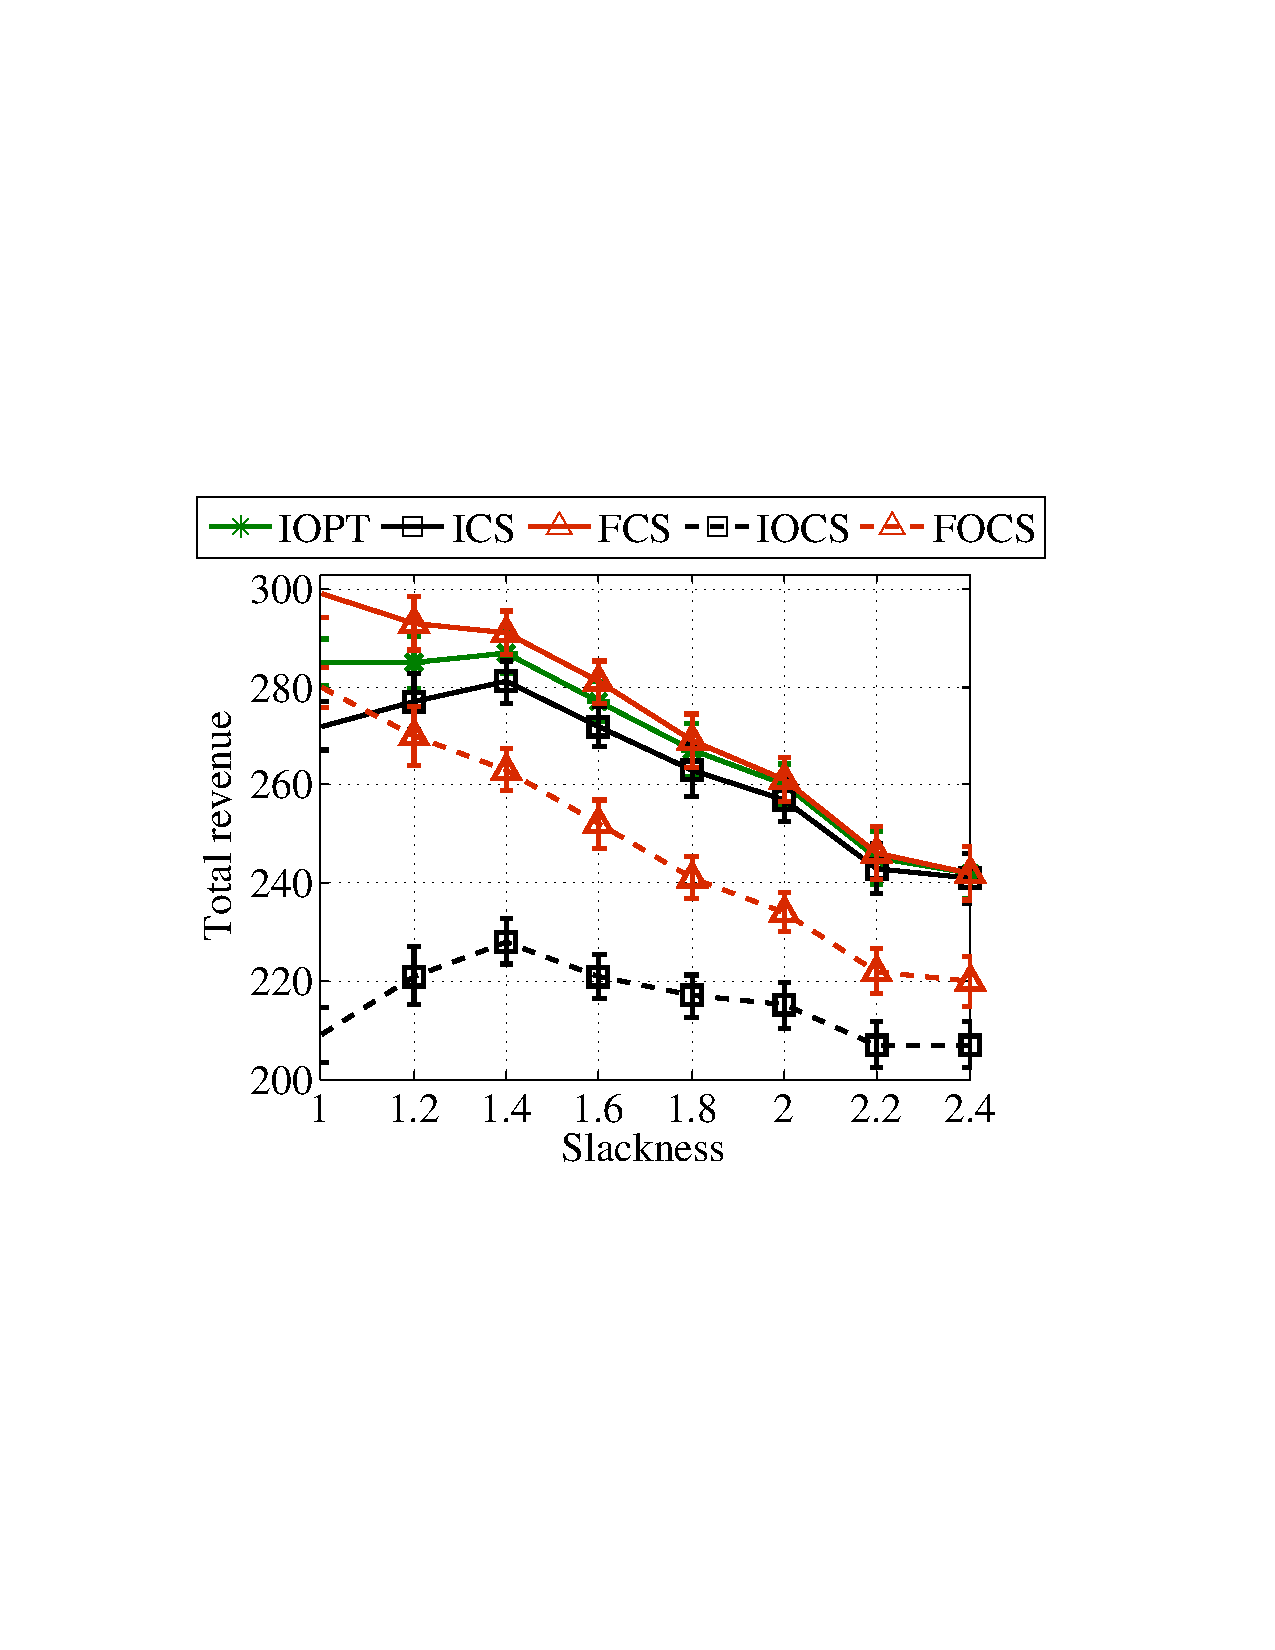
\includegraphics[width=\textwidth]{v-s-method1.pdf}
						\caption{Total revenue (\$)}
						\label{fig:v-s-method1}
					\end{center}
				\end{subfigure}%				
				\begin{subfigure}[b]{0.236\textwidth}
					\begin{center}
						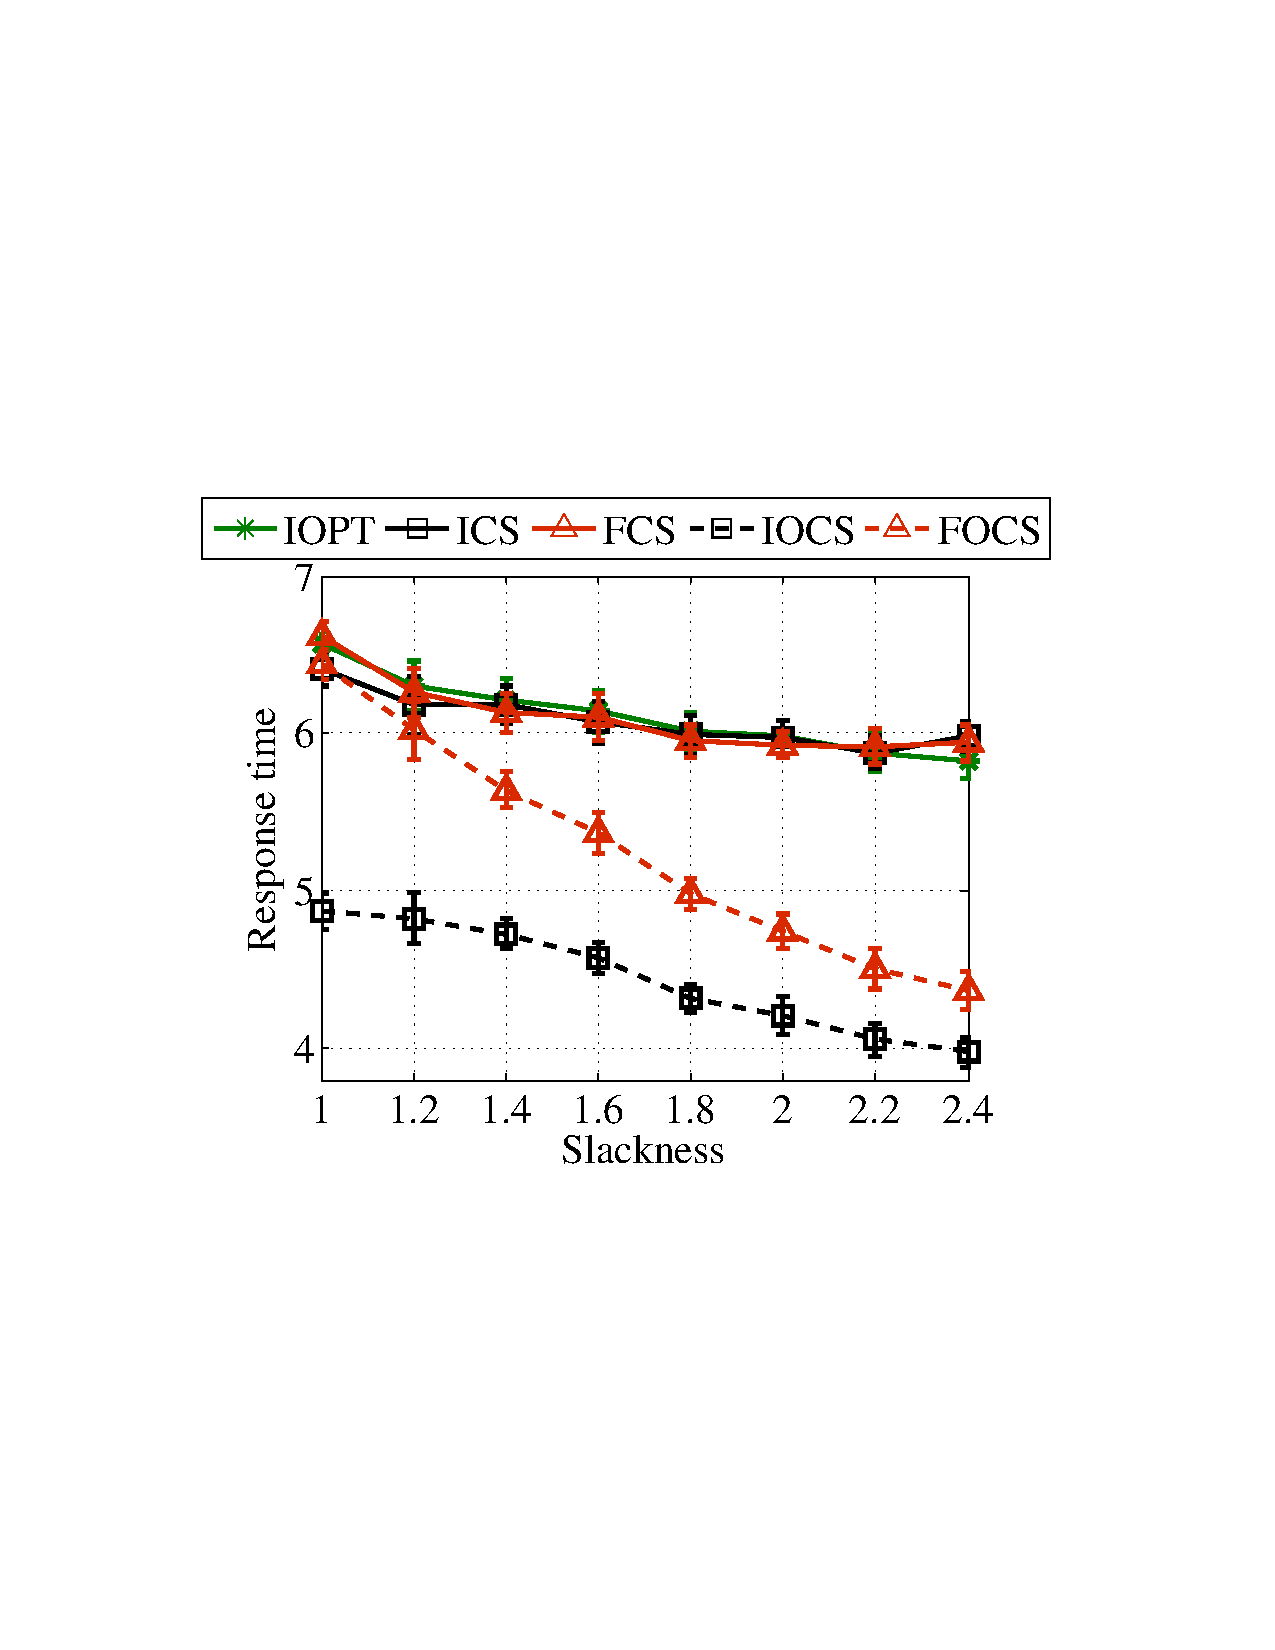
\includegraphics[width=\textwidth]{rt-s-method1.pdf}
						\caption{Response time (hr))}
						\label{fig:rt-s-method1}
					\end{center}
				\end{subfigure}%  
\caption{The impact of slackness parameter on total revenue and response time when users react by adjusting their demand.} 
\label{fig:slackness1}
\end{figure}
%\vspace{-1cm}

\begin{figure}[t]	
\vspace{-2mm}
\centering
							\begin{subfigure}[b]{0.236\textwidth}
								\begin{center}
									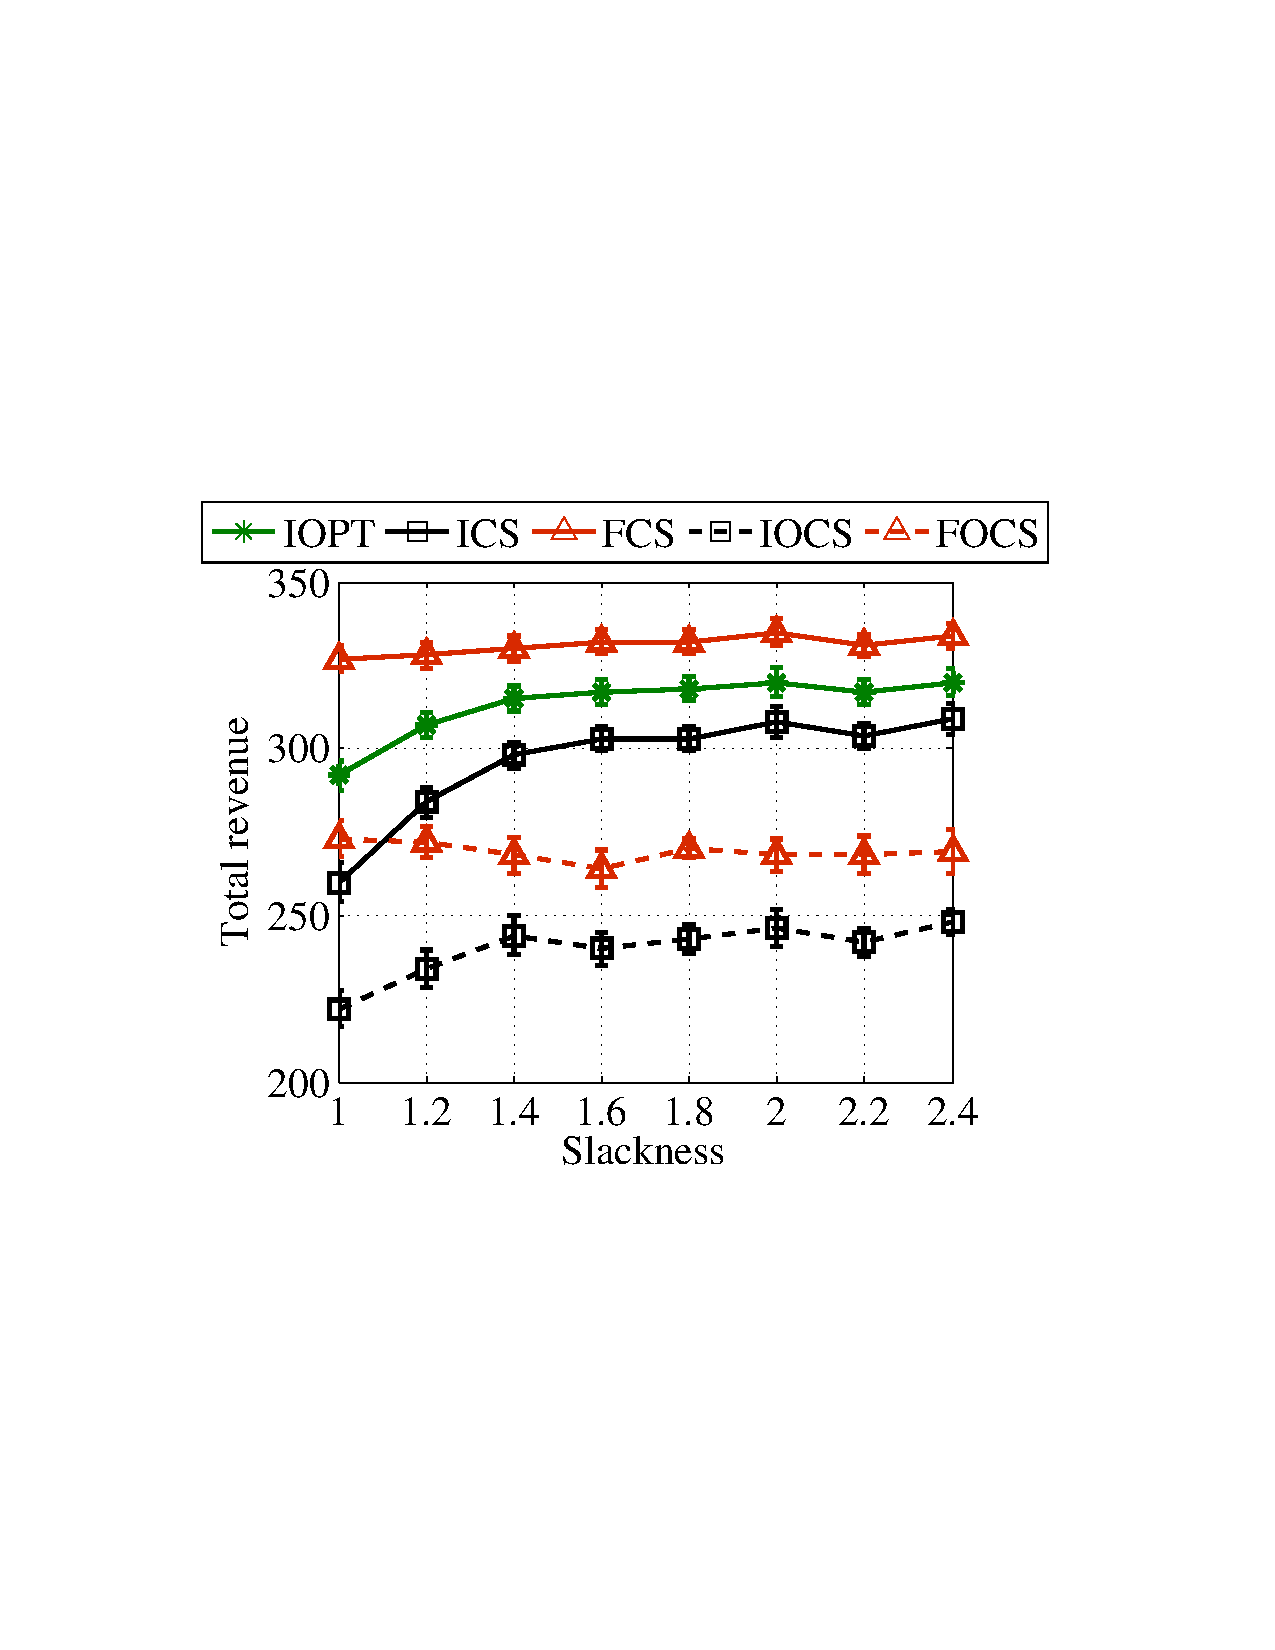
\includegraphics[width=\textwidth]{v-s-method2.pdf}
									\caption{Total revenue (\$)}
									\label{fig:v-s-method2}
								\end{center}
							\end{subfigure}%
							\hspace{1mm}
							\begin{subfigure}[b]{0.236\textwidth}
								\begin{center}
									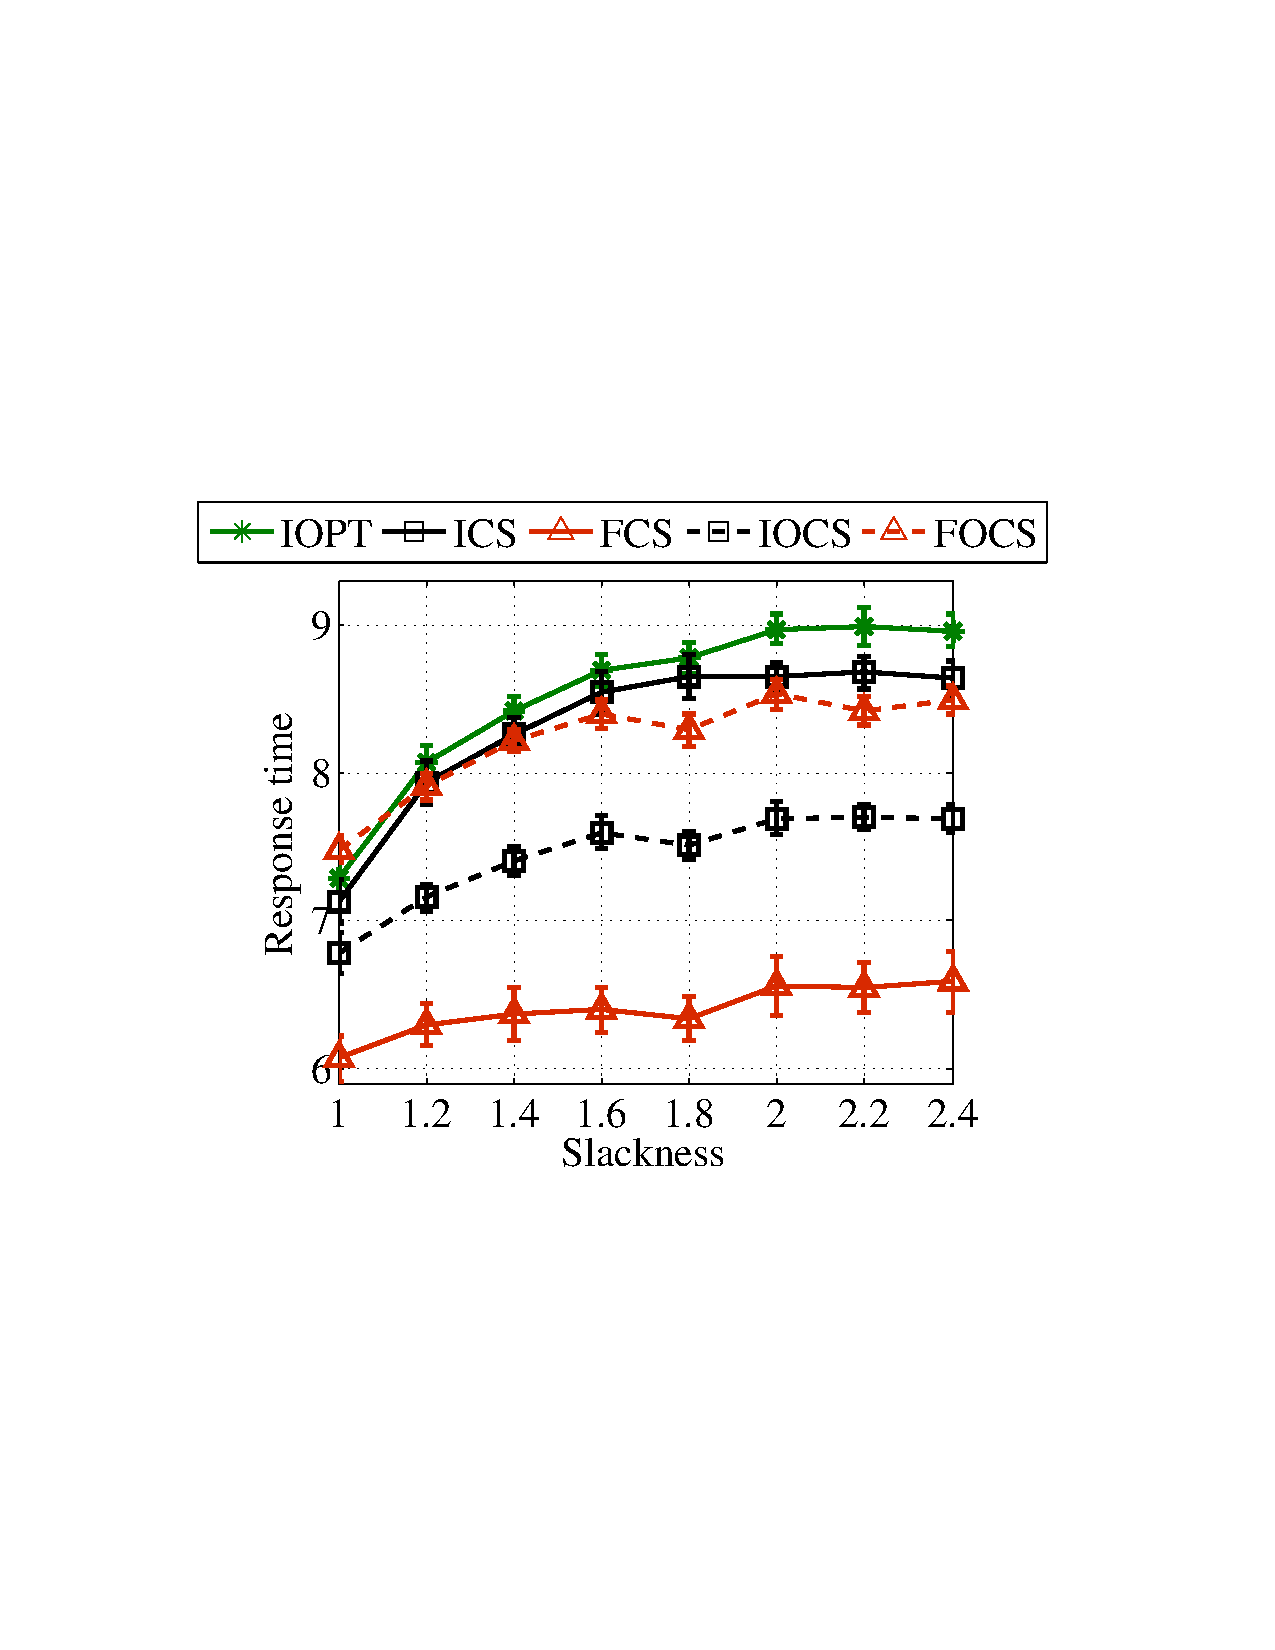
\includegraphics[width=\textwidth]{rt-s-method2.pdf}
									\caption{Response time (hr)}
									\label{fig:rt-s-method2}
								\end{center}
							\end{subfigure}% 
							
\caption{The impact of slackness parameter on total revenue and response time when users react by adjusting their deadline.} 
\label{fig:slackness2}
\end{figure}
			
\subsubsection{Case I- Adjusting Demands}
In this case, if the initial charging profile of an EV does not reflect a feasible charging request based on the slackness parameter, the EV owner decreases its demand so it will be able to leave CS at its initial desired deadline. Note that the valuation of EVs decreases proportionally, as well. Fig.~\ref{fig:slackness1} depicts the result under this policy applied by users. As it can be seen in Fig. \ref{fig:v-s-method1} and Fig. \ref{fig:rt-s-method1}, the general trend is that both total revenue and average response time decrease when slackness value increases. This is justifiable based on users reaction. When users decrease their demand, less electricity is sold which results in less revenue. When total demand decreases, charging can be finished in shorter time which decreases response time. Therefore, if users choose the first policy (adjusting their demand), total revenue degrades while response time improves. Notice that for the algorithms working under integral revenue model (i.e., \textsc{iOPT}, \ics and \iocs) the total revenue increases with slackness parameter at first (when $s$ grows from $1$ to $1.4$) but then it decreases when the slackness increases more (for $s>1.4$). 
In our view, this happens because increasing the slackness in integral revenue model makes it possible to \emph{fully} charge more EVs at the beginning as the demands decrease. However, when the slackness increases more, it results in opposite effect because the valuation of demands decreases along with the demands' size.	
			\subsubsection{Case II- Adjusting Deadlines}
			In this case, we assume that users are reluctant to decrease their desired demands. Instead, they can extend their departure. In Fig.~\ref{fig:slackness2} it can be observed that under this behavior of the users, the results are opposite as compared to the previous case (Fig.~\ref{fig:slackness1}). When deadlines are extended without demand decrement, the scheduler has more chance to compliance the demands through improved scheduling flexibility. Consequently, the total revenue increases by increasing slackness value while average response time degrades. 
%%Also observe the behavior of the online algorithms (i.e., \iocs and \focs) where both total revenue and response time decrease after a specific point that is $s=1.8$. When deadlines extend, more EVs have the opportunity of getting charged	
%					
We can conclude that when total revenue is more important than the response time, the CS should impose small values of slackness for users that apply the policy of the first case and impose higher values of slackness for the users that apply the second policy. The conclusion is reverse for the case that the objective is to have lower response times. 

			%In fact, the slackness parameter controls the maximum demand or earliest deadline that an EV can submit to the system. Remember that demands are in interval $[\textrm{min}\{\frac{d_i-a_i}{sk_i},U_i\},U_i]$ for EV $i$ meaning that the maximum demand that an EV can submit decreases by increasing slackness parameter. A reduction in total demand result in lower charging costs. Therefore, the total revenue decreases with higher values of parameter $s$ as in Fig. \ref{fig:v-s}. 
			%Also, the percentage of EVs that received all of their requested demand increases based on the same fact. The main goal of this simulation is to observe that obtained theoretical result on approximation ratio is confirmed as optimality gap of the SCS algorithm reduces by increasing $s$ in Fig. \ref{fig:v-s}. 

\end{comment}

\begin{comment}
\vspace{-10mm}
\begin{IEEEbiography}[{
\includegraphics[width=1in,height=1.25in,clip,keepaspectratio]{alinia.jpg}}]{Bahram Alinia} received a B.Sc degree in computer science from University of Tabriz, Tabriz, Iran and a masters degree in Information Technology Engineering from University of Tehran, Tehran, Iran. He was a Researcher with the School of Computer Science, Institute for Research in Fundamental Sciences, Iran, from 2009 to 2012. He is currently a Ph.D. student in service architecture lab, Institute Telecom SudParis, France and participated in several European projects in the domain of smart grids. His research area includes wireless communications, energy systems, transportation electrification, algorithm design and approximation.
\end{IEEEbiography}
%\vspace{-30mm}
\begin{IEEEbiography}[{
\includegraphics[width=1in,height=1.25in,clip,keepaspectratio]{hajiesmaili.jpg}}]{Mohammad H. Hajiesmaili} received the B.Sc. degree from the Department of Computer Engineering, Sharif University of Technology, Iran, in 2007, and the M.Sc. and Ph.D. degrees from the Electrical and Computer Engineering Department, University of Tehran, Iran, in 2009 and 2014, respectively. He was a Post-Doctoral Fellow with the Department of Information Engineering, the Chinese University of Hong Kong, from 2014 to 2016, and with the Department of Electrical and Computer Engineering, Johns Hopkins University, form 2017 to 2018. He is currently a Research Assistant Professor with the College of Information and Computer Sciences, University of Massachusetts, Amherst. His research interests include optimization, algorithm, and mechanism design in energy systems, electricity market, transportation networks, and multimedia networks.
\end{IEEEbiography}
%\vspace{-30mm}
\begin{IEEEbiography}[{
\includegraphics[width=1in,height=1.25in,clip,keepaspectratio]{crespi.jpg}}]{Prof. No\"{e}l Crespi} holds Masters degrees from the Universities of Orsay (Paris 11) and Kent (UK), a diplome d'ing\'{e}nieur from Telecom ParisTech, a Ph.D and an Habilitation from UPMC (Paris-Sorbonne University). From 1993 he worked at CLIP, Bouygues Telecom and then at Orange Labs in 1995. He took leading roles in the creation of new services with the successful conception and launch of Orange prepaid service, and in standardisation (from rapporteurship of IN standard to coordination of all mobile standards activities for Orange). In 1999, he joined Nortel Networks as telephony program manager, architecting core network products for EMEA region. He joined Institut Mines-Telecom in 2002 and is currently professor and Program Director, leading the Service Architecture Lab. He coordinates the standardisation activities for Institut Mines-Telecom at ITU-T and ETSI. He is also an adjunct professor at KAIST (South Korea), an affiliate professor at Concordia University (Canada), and gest researcher at the University of Goettingen (Germany). He is the scientific director the French-Korean laboratory ILLUMINE. His current research interests are in Data Analytics, Internet of Things and Softwarisation.
http://noelcrespi.wp.tem-tsp.eu/
\end{IEEEbiography}	
\end{comment}
\end{document}
